\chapter{Results and discussion}\label{ch:results}
%%%%%%%%%%%%%%%%
%- Introduction of what we are looking for, reminder of hypothesis
%%%%%%%%%%%%%%%%
Data from previous experiments \cite{Bostedt-2012-PRL,Gorkhover-2016-NatPho,Ferguson-2016-SciAdv}, where diffraction images and time-of-flight data were recorded in coincidence, show that the diffraction images carry transient information about the nanoplasma formation and expansion. The time-of-flight spectra contain valuable information about the atomic ionization as well as expansion dynamics from large ionized clusters and are therefore briefly discussed first in Section \ref{sec:itof-pump--probe}. The scattering response of the clusters to intense X-ray pulses is discussed in the following in Section \ref{sec:scattering-response}.\\[1\baselineskip]
%All data taken with coincident measurement of time-of-flight data and diffraction imaging in previous experiments  show that the diffraction images carry transient information of the nanoplasma formation and expansion during the pulse and are therefore the focus of the following discussion. However, the time-of-flight spectra contain valuable information about the atomic ionization as well as large ionized cluster expansion dynamics  This chapter is thus organized as follows: 
%
For the hasty reader the organization of the subsections may be helpful: Section \ref{sec:time-resolved-xe-atoms} discusses the time dependent response of Xe-atoms and -clusters to X-ray pump--X-ray probe beams in the ion TOF data. Section \ref{sec:hexe--and-he-TOF} continues the ion TOF data discussion on superfluid He- and mixed HeXe-clusters. Section \ref{sec:xenon-data} covers the scattering response of pristine Xe-clusters. Section \ref{sec:He-data-real} discusses the nanoplasma expansion of He-clusters in intense X-rays. Section \ref{sec:helium-data} addresses the agglomeration of heterogeneous HeXe-clusters and introduces the plum-pudding cluster model. Section \ref{sec:helium-xenon-data} discusses sample damage in HeXe-clusters using 2D-simulations. Section \ref{sec:comparison-of-He-and-HeXe-clusters} compares radiation damage of Xe-, He- and HeXe-clusters in intense X-rays to each other.\\[1\baselineskip]
%Section \ref{sec:itof-pump--probe} discusses the ion time-of-flight pump--probe data.
%First, the nanoplasma transition in pristine Xe-clusters is discussed in Section \ref{sec:xenon-data}. 
%The arrangement of Xe-atoms in HeXe-clusters is discussed in Section \ref{sec:helium-data} using 2D-simulations. Sample damage scenarios of HeXe-clusters are compared to simulations in Section \ref{sec:helium-xenon-data}. Section \ref{sec:comparison-of-He-and-HeXe-clusters} compares structural damage from the nanoplasma expansion for the different samples, He-, Xe-, and HeXe-clusters, to each other.\\[1\baselineskip]
%
The X-ray pulse parameters of this study are summarized in Table \ref{tab:beam-params} on Page \pageref{tab:beam-params}. It should be noted again that the split of the multipulse energy is \SI{10}{\percent} in the pump-pulse and \SI{90}{\percent} in the probe-pulse. This allows us to neglect the contributions of the pump-pulse to the scattering images (see Section \ref{sec:pump--probe-considerations}).
%The below discussed X-ray pump--X-ray probe data carries data from strictly speaking both pulses. Due to the split of the overall pulse energy in \SI{10}{\percent} to the pump-pulse and \SI{90}{\percent} to the probe-pulse, the contributions from the pump-pulse can be disregarded (see Section \ref{sec:pump--probe-considerations}).
%
%
%%%
\section{Ion time-of-flight X-ray pump--X-ray probe data}\label{sec:itof-pump--probe}
\subsection{Time-dependent response of Xe-atoms and -clusters to intense X-rays}\label{sec:time-resolved-xe-atoms}
%%%%%%%%%%%%%%%%%%%%%%%%%%%%%%%%%%%%%%%%%
%- Xe iToF dynamics\\
%- Slightly more of Xe higher charge-states present at longer delays.
%%%%%%%%%%%%%%%%%%%%%%%%%%%%%%%%%%%%%%%%%
\begin{figure}
	\centering
		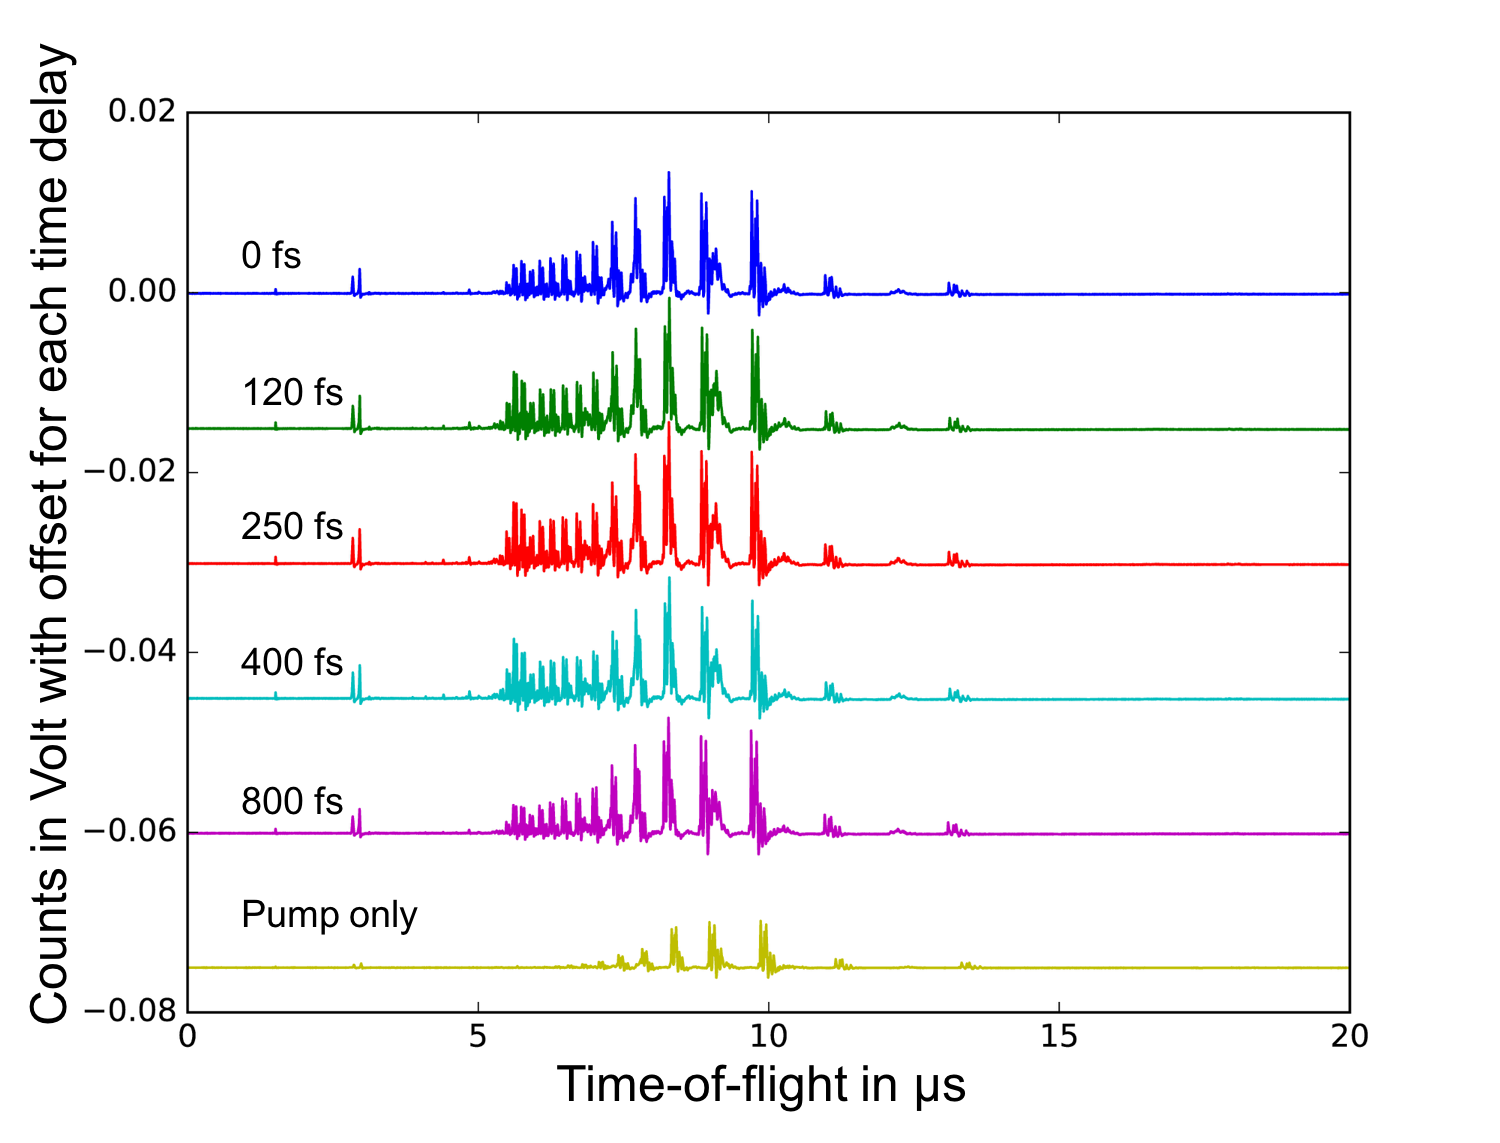
\includegraphics[width=0.65\textwidth]{images/results/TOF-atomic-xenon2.png}
	\caption[Time-resolved answer of xenon atoms in TOF spectroscopy.]{Time-resolved answer of xenon atoms in TOF mass spectroscopy. The Xe-atom response to the X-ray pump--X-ray probe pulses from LCLS shows a resonant behavior in the high-charge states that peak at \SI{\sim250}{\femto\second} (see also Figure \ref{fig:TOF-atomic-xenon-time-dependent}).}
	\label{fig:TOF-traces-xenon-atoms}
\end{figure}
For the interpretation of the dynamic data from Xe- and HeXe-clusters it is first important to establish how individual atoms respond to a X-ray pump--X-ray probe experiment. Ion time-of-flight traces of atomic xenon at various time delays $\Delta t =$ \SIlist{0;120;250;400;800}{\femto\second} and X-ray pump-pulse only data are shown in Figure \ref{fig:TOF-traces-xenon-atoms}. All TOF traces below are averages of the \SI{\sim 10}{\percent} most intense hits of the respective run. The time-of-flight data indicate a resonant-like behavior in the time-domain as the atomic xenon high-charge states peak at $\Delta t\approx$ \SI{250}{\femto\second} with a clear increase. This is also shown in Figure \ref{fig:TOF-atomic-xenon-time-dependent}, where the total high-charge state ion-yield for Xe-atoms between the TOF range \SIrange{5.13}{6.50}{\micro\second} is plotted as a function of the time delay, $\Delta t$. The charge-state composition is highly dependent on the X-ray absorption process. For highly intense X-ray pulses, absorption is a complicated process involving multi-photon core-hole excitations and decay processes. Further theoretic investigations are needed to explain the spectra in more detail \cite{Ho-2014-PRL,Ho-2016-PC}. However, this resonant-like effect could be related to intensity-induced X-ray transparency \cite{Young-2010-Nature,Schorb-2012-PRL}. In this thesis experiment, the xenon 3d-subshell is efficiently photoionized by the X-ray pump-pulse. The resulting electron-holes in the 3d-subshell are typically repopulated on the few femtoseconds timescale due to the Auger decay, but the increasingly ionized atoms have also increasingly longer hole lifetimes, for example, previous studies show that $\text{Ne}^{8+}$ has core-hole lifetimes of \SI{\sim230}{\femto\second} \cite{Young-2010-Nature} making the atom increasingly transparent during the vacancy lifetime. In the present case, the absorption of photons from the probe-pulse is suppressed for delays $\Delta t \leq \SI{120}{\femto\second}$ because of this transparency. When the delay is $\Delta t = \SI{250}{\femto\second}$, the xenon 3d-subshell repopulates and the probe-pulse can efficiently photoionize the 3d-subshell again. But, why does the charge state distribution not level out for later delays $\Delta t >$ \SI{250}{\femto\second}? When the strongly pumped atom does not absorb energy near saturation, decay processes catch up and the nanoplasma dissipates energy in surrounding media. Subsequent recombination then could lead to less intense high-charge state populations.\\[1\baselineskip]
%
\begin{figure}
	\centering
	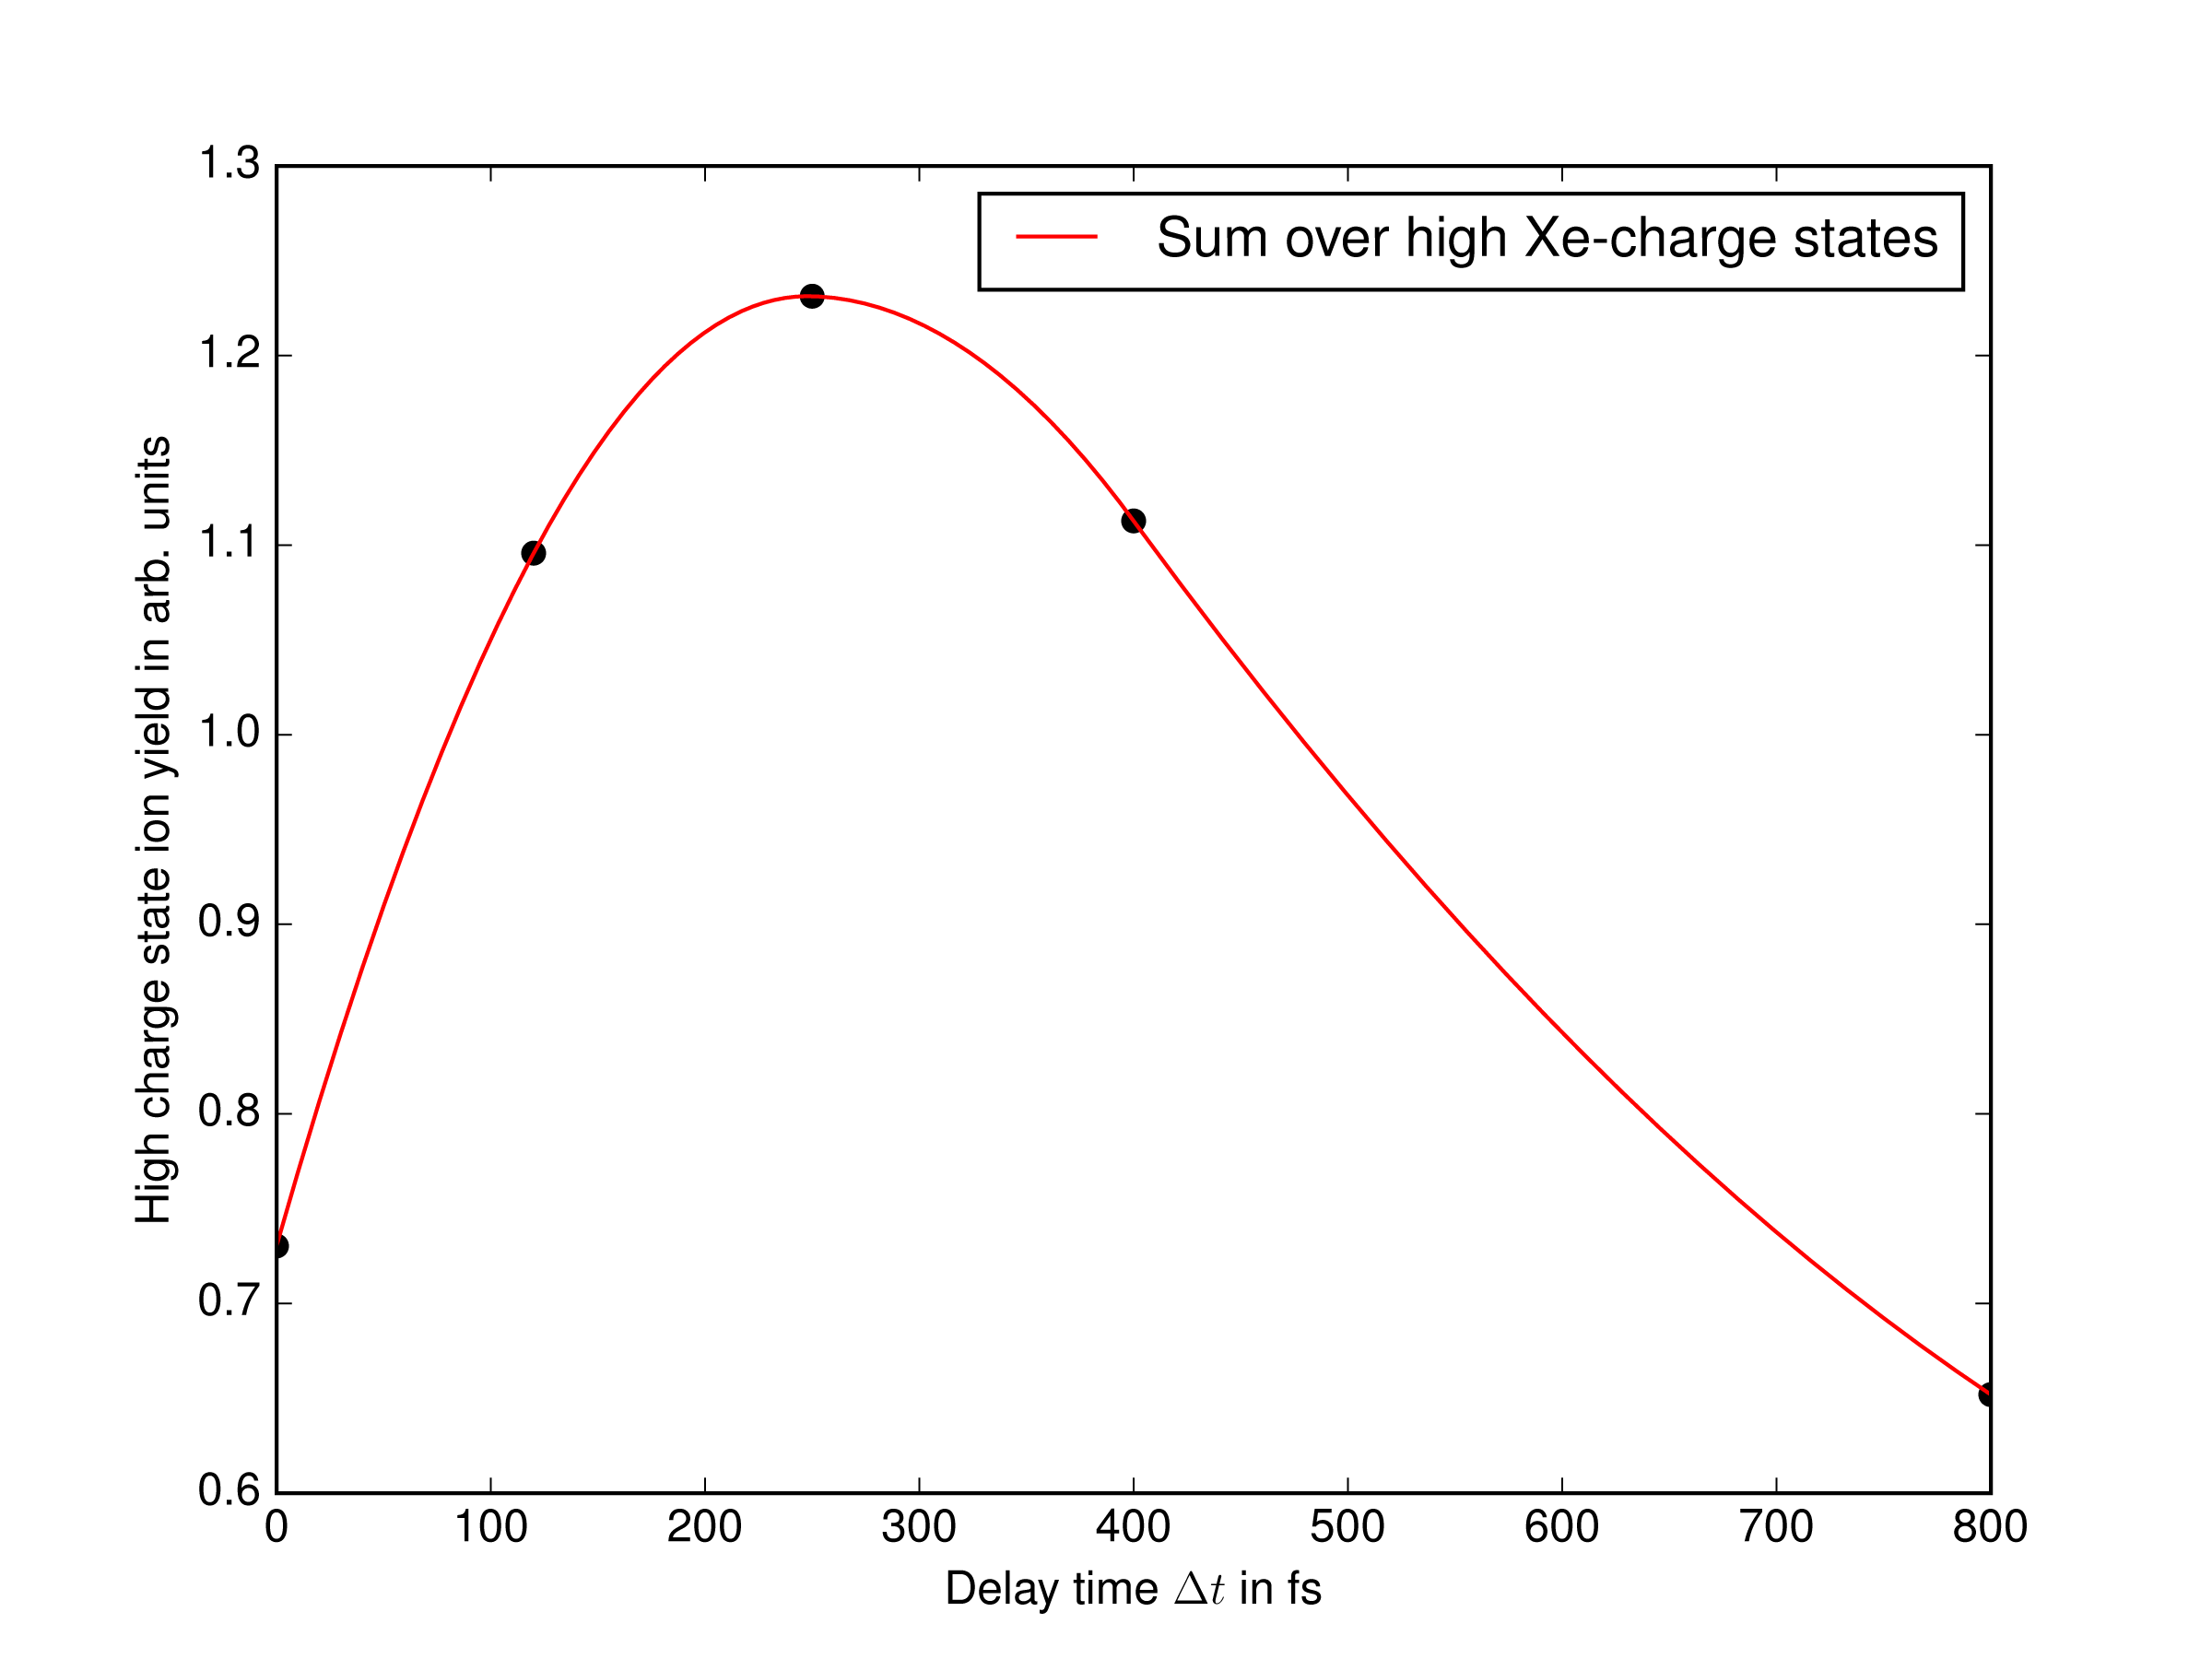
\includegraphics[width=0.6\textwidth]{images/results/atomic-charge-state-time-resolved.png}
	\caption[Time-dependent response of atomic xenon in TOF spectroscopy.]{The total of the high-charge state ion-yield for Xe-atoms between the TOF range \SIrange{5.13}{6.50}{\micro\second} or $(\sim \text{Xe}^{17+} \text{to } \text{Xe}^{10+})$ as a function of the time delay, $\Delta t$. The atomic Xe-ion TOF data show resonant behavior. As the time delay is varied in the range $\Delta t=$ \SIrange{0}{800}{\femto\second}, the high-charge states of atomic Xe-ions peak at \SI{\sim250}{\femto\second}.}
	%As the X-ray pump-pulse traverses through the xenon ions, the 3d-subshell becomes highly ionized and thus the atom becomes increasingly transparent for the probe-pulse ($\Delta t \approx$ \SIrange{0}{120}{\femto\second}). The electron-holes have a longer lifetime due to the highly ionized subshell. After the Auger decay populates the 3d-subshell, the atom becomes less transparent and the X-ray probe-pulse efficiently ionizes the atoms ($\Delta t \approx \SI{250}{\femto\second}$). Eventually, relaxation processes dissipate energy leading to fewer high-charge states ($\Delta t < \SI{400}{\femto\second}$).}
	\label{fig:TOF-atomic-xenon-time-dependent}
\end{figure}
%
%This makes the Xe-atoms become increasingly transparent 
%as the X-ray pulse propagates.
%The xenon high-charge states start low at $\Delta t = 0$ fs and then peak due to intensity-induced X-ray transparency \citep{Young-2010-Nature,Schorb-2012-PRL}. 
%In the present study, the xenon 3d-subshell is efficiently ionized by the X-ray pump-pulse. These electron-holes are typically repopulated on the few femtosecond timescale due to the Auger decay, however, the increasingly ionized atom has longer electron-hole lifetimes and the Xe-atoms become increasingly transparent as the X-ray pulse propagates. It has been measured that $\text{Ne}^{8+}$ has core-hole lifetimes of $~230$ fs. 
%
%
%
%The left panel of Figure \ref{fig:TOF-small-cluster-xenon} shows ion time-of-flight traces of small xenon cluster at different time delays $\Delta t =$ \SIlist{0;120;250;400;800}{\femto\second} and X-ray pump-only data. The xenon cluster in this data-set have an average radius of \SI{\sim 3.5}{\nano\meter}. The right panel of Figure \ref{fig:TOF-small-cluster-xenon} compares the total high-charge state ion yield for Xe-atoms and Xe-clusters and the dashed-lines are bspline fits to help the eye. For the \SI{\sim 3.5}{\nano\meter} radius Xe-cluster, the high-charge state time-dependence becomes increasingly complex. A theoretic study of these effects is beyond the focus of this work. However, the experimental data indicates that for shorter time delays, $\Delta t<$\SI{\sim 400}{\femto\second}, the time-dependency could be similar to the one of Xe-atoms. At longer time-delays, $\Delta t<$\SI{\sim 400}{\femto\second}, the high-charge state signal overall increases. This can be attributed to the expanding cluster and thus resulting lowering in Coulomb potential (see Figure \ref{fig:nano-plasma-schematic}) \cite{Krikunova-2009-NJP}. A further theoretic investigation that is beyond the scope of this thesis and typically requires access to supercomputers such as MIRA is needed and ongoing \cite{Ho-2016-PC}.\\[1\baselineskip]
%\begin{figure}
%	\centering
%		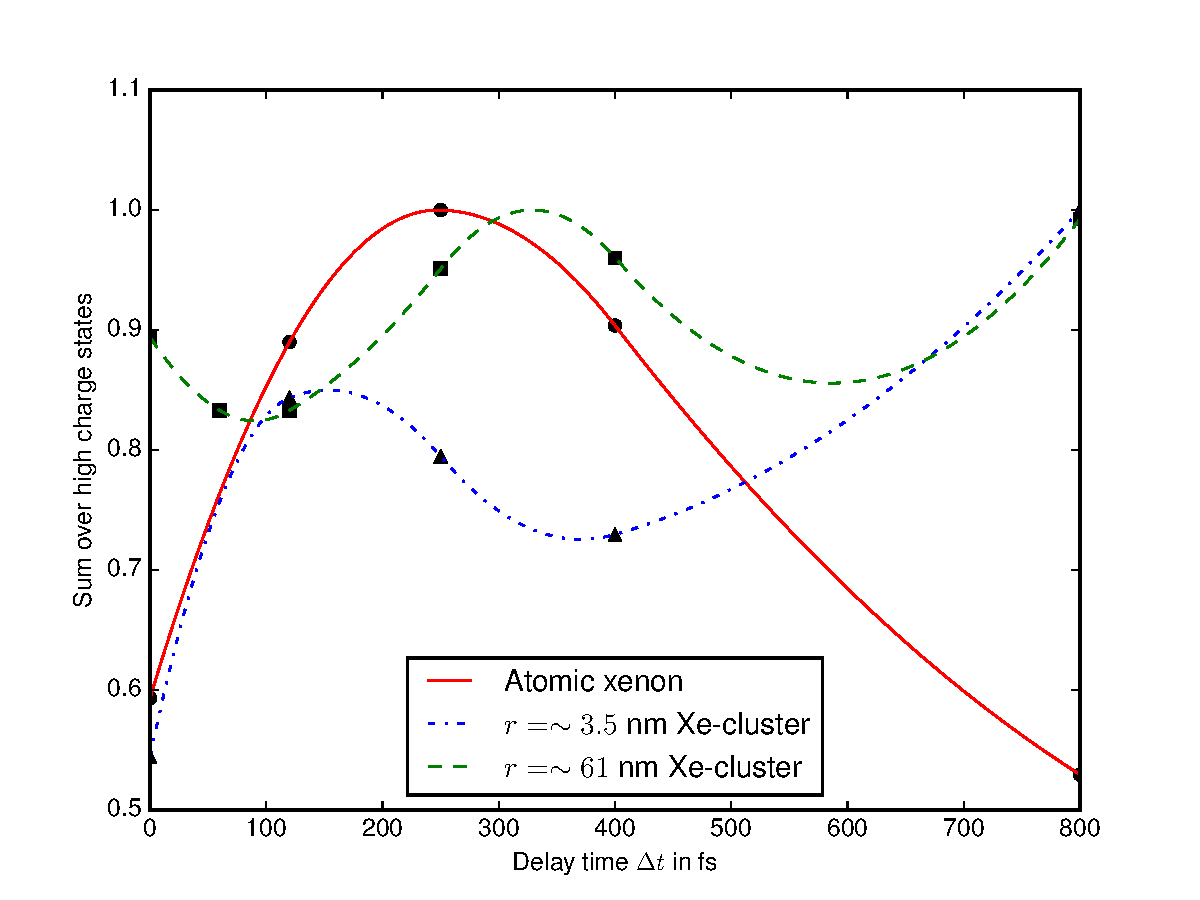
\includegraphics[width=0.49\textwidth]{images/results/clusterSummary_all}
%	\caption{caption}
%	\label{fig:TOF-regular-cluster-xenon}
%\end{figure}
The response of clusters to highly intense X-ray radiation is more complex. Size-dependent ionization \citep{Schorb-2012-PRL,Schutte-2015-JPhysB} and recombination in the nanoplasma \citep{Schutte-2014-PRL} alter the sample's ionization pathways. Ion time-of-flight traces of Xe-clusters are displayed in Figure \ref{fig:TOF-traces-xenon-cluster}. The time delay has been set to $\Delta t=$\SIlist{0;60;120;250;400;800} and also the pump only data is shown. The mean radius of the initially injected Xe-clusters are \SI{\sim 61}{\nano\meter} but they will expand by \SI{\sim20}{\percent} over a $\Delta t$ range of \SIrange{0}{800}{\femto\second} as discussed later in Section \ref{sec:xenon-data}. Unlike the atomic xenon data, the Xe-clusters show no clear resonant-like effect. The Xe-cluster data indicate a weak time-dependence of ionization and with increasing $\Delta t$, the high-charge states overall increase. This can be attributed to the expanding cluster. During the expansion, the cluster potential lowers \cite{Arbeiter-2011-NJP} and the electron transition dynamics become more complex \cite{Krikunova-2009-NJP}. To describe the time-dependent ionization of clusters in detail, a theoretic investigation that is beyond the scope of this thesis is needed and ongoing \cite{Ho-2016-PC}.
%owers the Coulomb potential (see Figure \ref{fig:nano-plasma-schematic}) and the more complex electron recombination possibilities \cite{Krikunova-2009-NJP}.
%For the \SI{\sim 61}{\nano\meter} radius Xe-cluster, the high-charge state time-dependence becomes increasingly complex. A theoretic study of these effects is beyond the focus of this work. However, the experimental data indicates that for shorter time delays, $\Delta t<$\SI{\sim 400}{\femto\second}, the time-dependency could be similar to the one of Xe-atoms. At longer time-delays, 
%The data show that the cluster type of signal is dominating the trace. At a time delay $\Delta t=800$ fs, the xenon high-charge states increase, while no other dynamic appears obvious from the average data. The larger cluster ensemble may undergo a similar resonant type behavior as atomic xenon, however, the large cluster ensemble seem to affect the ionization pathways and thus the timescale of the resonant type behavior.\\[1\baselineskip]
%
%Summarizing, atomic xenon, xenon cluster of mean radius $\sim XXX$ nm and Xe-cluster of average radius $\sim 61$ nm were investigated using an X-ray pump--X-ray probe setup coincidentally measuring spectroscopy and coherent diffractive imaging data. The ion spectroscopy data of atomic xenon high-charge states show a resonant type behavior as the time delay $\Delta t$ is varied from 0 fs to 800 fs. The effect peaks, i.e. is resonant around 250 fs. Small xenon cluster exhibit a similar behavior as atomic signal because atomic signal is dominating the high-charge states. The signal from larger xenon cluster of radii $\sim 61$ nm is dominated by xenon charge fragments. An increase in the xenon high-charge states is observed at 800 fs, allowing us to conclude that the ionization dynamics have changed. It is interesting to note that altough larger cluster absorb overall more energy, the ensemble of atoms that is bound in the cluster is able to collectively change, here slow, ionization pathways. This behavior may be reproduced in other nano-samples such as bio-molecules or artifical tamper layers.
\begin{figure}
	\centering
		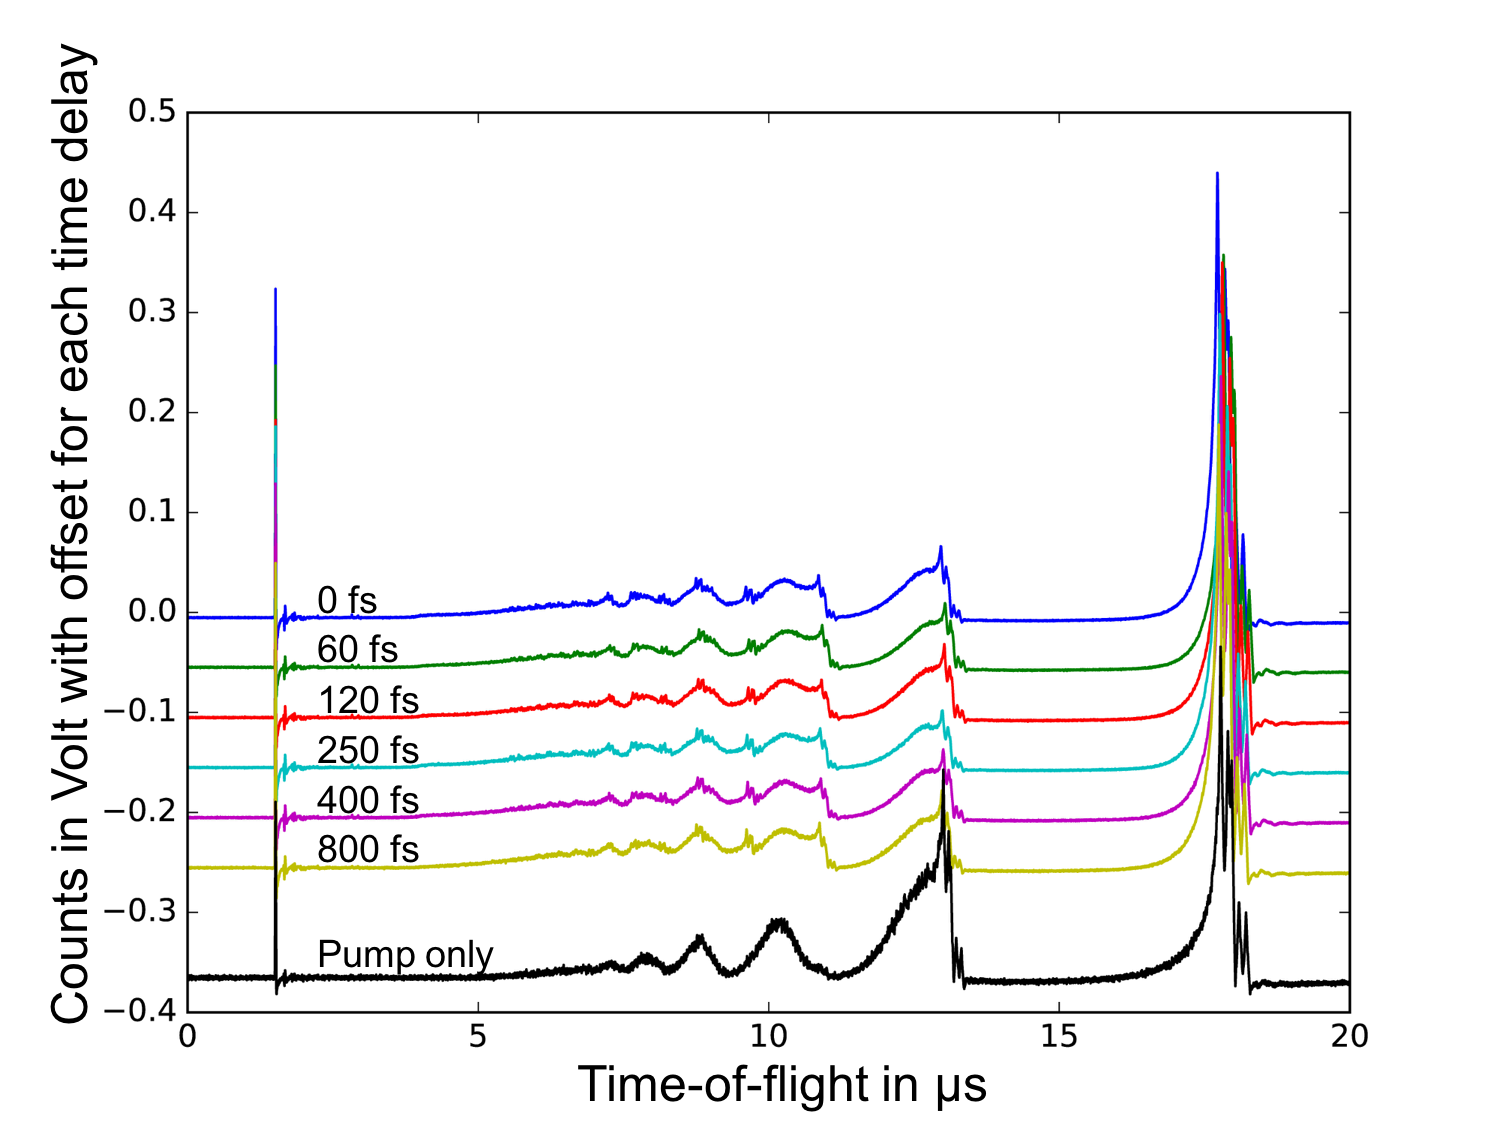
\includegraphics[width=0.65\textwidth]{images/results/TOF-regular-cluster-xenon2.png}
	\caption[Time-resolved answer of xenon clusters in TOF spectroscopy.]{Time-resolved answer of xenon clusters in TOF mass spectroscopy. Unlike the atomic response, Xe-clusters show no clear resonance and overall have a weak time dependence.}
	\label{fig:TOF-traces-xenon-cluster}
\end{figure}
%
%
%
%%%%%%%%%%%%%%%%%%%%%%%%%%%%%%%%%%%%%%%%
\subsection[Time-resolved response of highly ionized He- and HeXe-clusters]{Time-resolved response of He- and HeXe-clusters in intense X-rays}\label{sec:hexe--and-he-TOF}
%%%%%%%%%%%%%%%%%%%%%%%%%%%%%
% - Subsection for iToF data, important to compare to HeXe data.
%%%%%%%%%%%%%%%%%%%%%%%%%%%%%
\begin{figure}
	\centering
		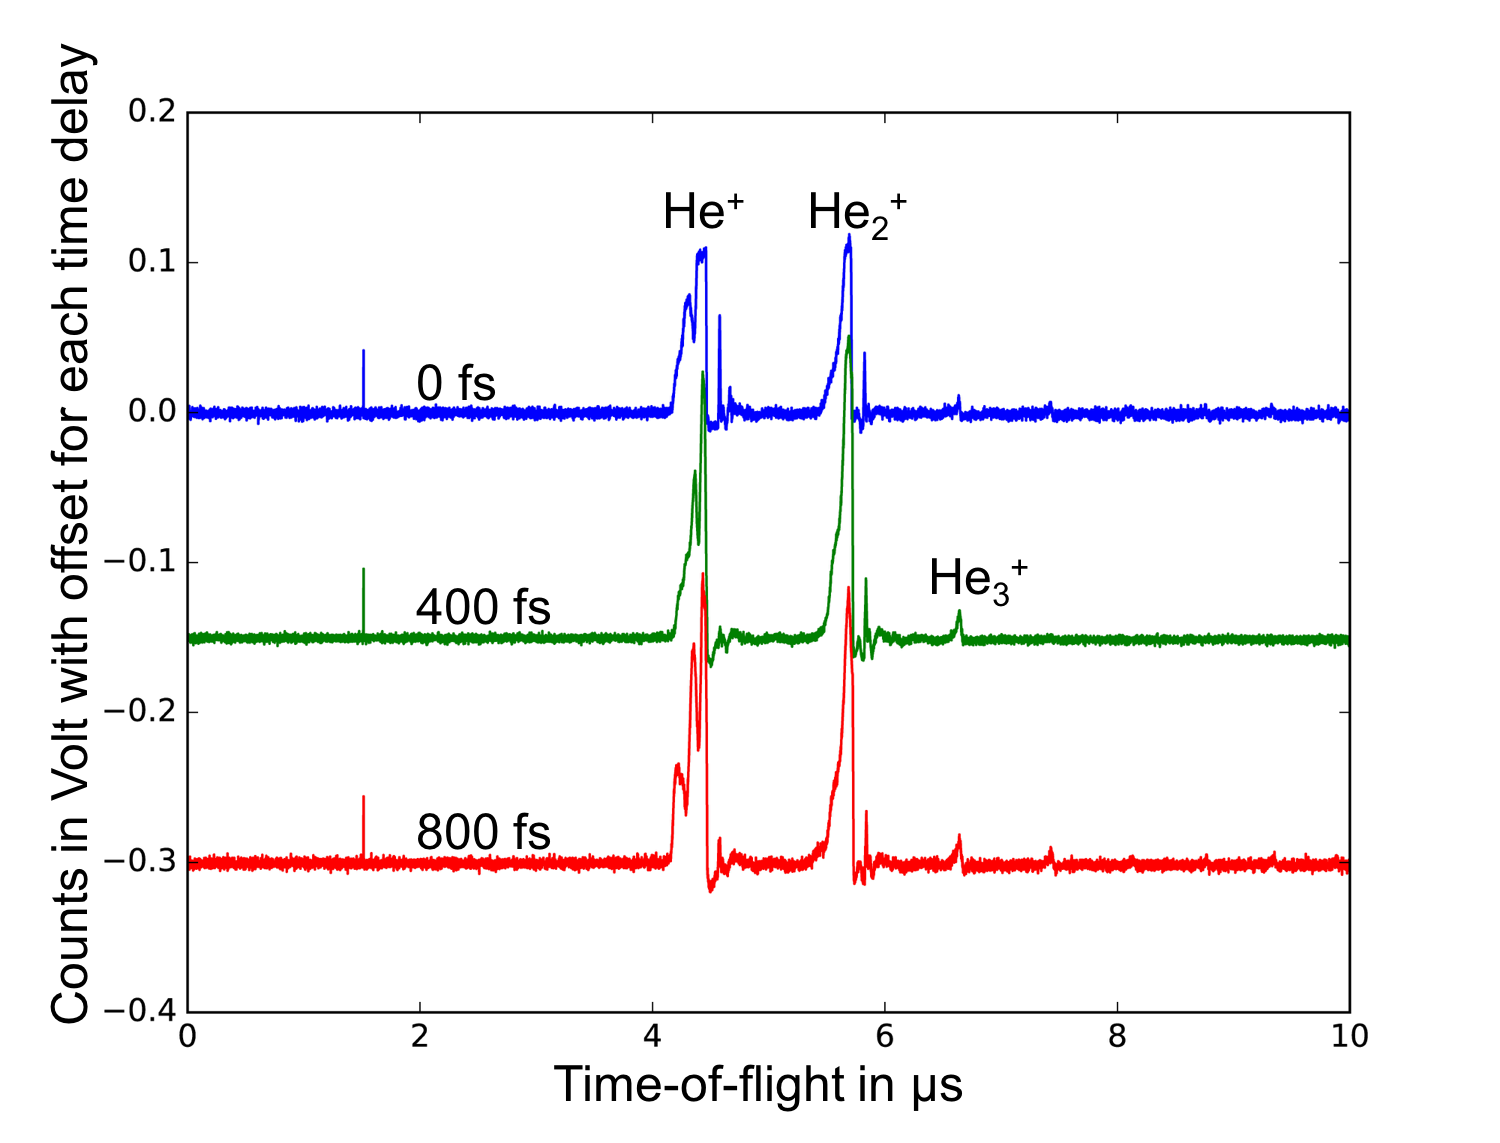
\includegraphics[width=0.65\textwidth]{images/results/TOF-helium-cluster2.png}
	\caption[Time-resolved answer of He-clusters in TOF spectroscopy.]{Ion time-of-flight traces of He-cluster with a radius of $r_{\text{He}}\approx \SI{810}{\nano\meter}$. Although minor changes in the charge fragmentation are observed, we shall note that there are no He$^{2+}$ ions in this data. The absorption cross-section of helium are too low to lead to doubly-charged states \citep{Ho-2016-PC}.}
	\label{fig:TOF-helium-cluster}
\end{figure}
%
He-droplets exhibit a weak response to the X-ray pump--X-ray probe delay similar to the Xe-cluster. Figure \ref{fig:TOF-helium-cluster} shows ion time-of-flight data of pristine He-cluster at pump--probe delays $\Delta t=$ \SIlist{0;250;800}{\femto\second}. The pristine He-droplets have an average radius of $r_{\text{He}}\approx$ \SI{810}{\nano\meter} that has been derived from the cluster growth scaling laws (see Section \ref{sec:homogenous-cluster}). The data show an overall similar behavior regardless of the delay $\Delta t$, although minor changes in the charge fragmentation distribution can be seen. The He-data is shown for comparison to the HeXe-cluster data presented below. For the comparison, it is important to note that the TOF traces indicate no contribution of doubly-charged helium atoms. The lack of double-charged helium can be explained by the comparably low absorption cross-sections of helium (see Table \ref{tab:helium-xenon-ionization}) \cite{Ho-2016-PC}.\\[1\baselineskip]
%
\begin{figure}
	\centering
		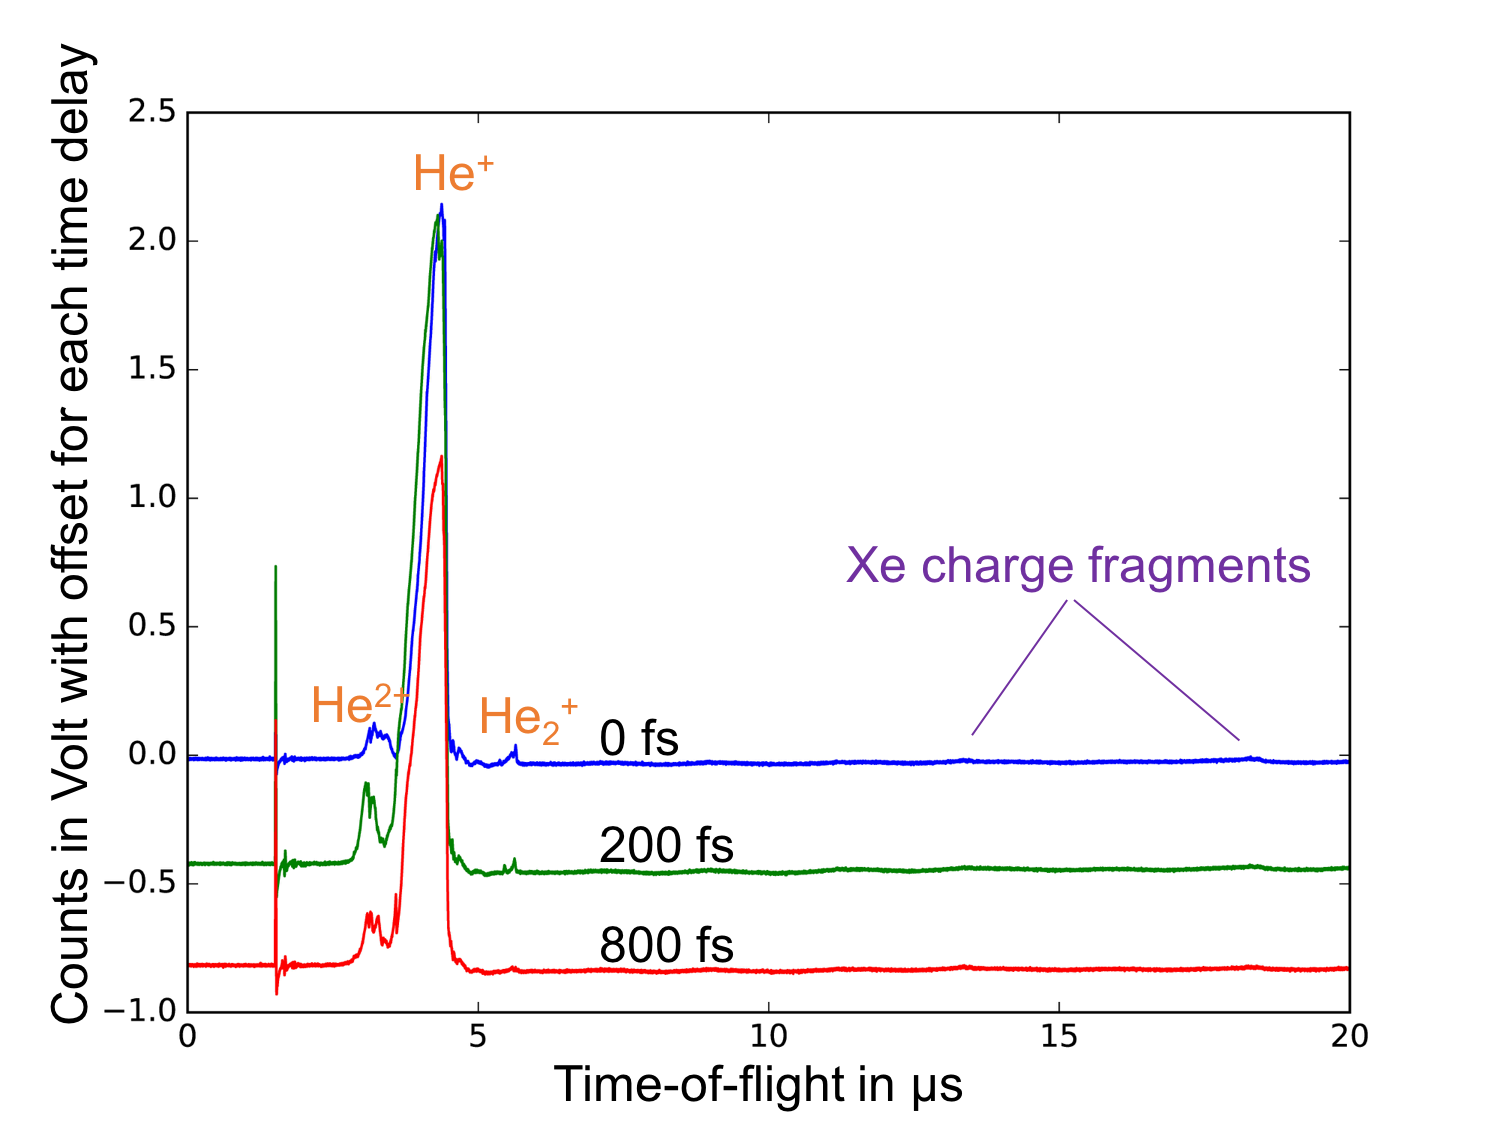
\includegraphics[width=0.65\textwidth]{images/results/TOF-helium-xenon-cluster-60-2.png}
	\caption[TOF spectra of HeXe-clusters with a \SI{\sim 0.6}{\percent} Xe-doping at various $\Delta t$.]{Ion TOF spectra of HeXe-cluster with radius $r\approx$ \SI{600}{\nano\meter} and a Xe-doping level of \SI{\sim 0.6}{\percent}. Only neglible contributions from Xe-charge-fragments are observed. Conversely, doubly-charged He$^{2+}$-ions are detected and the kinetic energy release of the He-peaks varies. With increasing delay time, the He-ions reveal a time-dependence.}
	\label{fig:TOF-helium-xenon-cluster-60}
\end{figure}
%
Next, HeXe-cluster with a radius of $r_{\text{He}}\approx$ \SI{600}{\nano\meter} and a \SI{\sim 0.6}{\percent} doping level of xenon are discussed. For clarity, this is measured through the helium depletion measurement, which was discussed in Section \ref{sec:heterogeneous-cluster}. At this doping level, the helium depletion is \SI{\sim 62}{\percent}. The TOF spectra are shown in Figure \ref{fig:TOF-helium-xenon-cluster-60} for the delays, $\Delta t=$ \SIlist{0;200;800}{\femto\second}. Most notable is the presence of $\text{He}^{2+}$ ions and the strongly increased signal from $\text{He}^{+}$ ions. But, only few xenon charge fragments are observed. This is counter-intuitive as the absorption cross-section from xenon is much larger than from helium (see Table \ref{tab:helium-xenon-ionization}). We can therefore hypothesize that ultrafast charge-transfer occurs between the Xe-particles and the He-droplets \cite{Hoener-2008-JPB}. The He-droplet functions as electron reservoir for the Xe-clusters and therefore they can recombine. The neutral Xe-particles are not detected by the ion TOF spectrometer and barely any signal of Xe charge fragments is detected \cite{Hoener-2008-JPB,Hau-Riege-2007-PRL}. The absence of Xe charge fragments indicates also the sample integrity of the Xe-particles. As we look at the longer delays $\Delta t$, it is interesting that the He-ion signals of the HeXe-clusters show a strong time-dependence. Similar to the atomic xenon data, we observe that the He-ion signal shows a resonant-type behavior and at $\Delta t =$ \SI{200}{\femto\second}, the signals from $\text{He}^{2+}$ and $\text{He}^{+}$ peak. We can make use of the earlier discussion around the data shown in Figure \ref{fig:TOF-atomic-xenon-time-dependent} and \ref{fig:TOF-helium-cluster} and conclude that this resonant-like behavior does not originate from the absorption and ionization dynamics of the He-droplet but rather from the Xe-atoms with which the He-droplet is doped. This allows us to hypothesize that there must be an ultrafast kinetic energy transfer process as charge-transfer alone does not explain the increase in kinetic energy of the He-ions \cite{Hoener-2008-JPB,Sugishima-2012-PRA,Muller-2015-JPhysB}. For example, collisions could transfer energy from the Xe-particles to the He-droplet. This thought can be expanded and it is theoretically predicted that electron-electron collisions of trapped electrons in the cluster potential occur frequently \cite{Arbeiter-2011-NJP}. These collisions could be responsible for this energy exchange. This indication of trapped electrons is interesting because these electrons damage the sample due to secondary collisional ionization \cite{Hau-Riege-2004-PRE} and we will discuss some implications for diffractive imaging below. Note that the He-dimer signal decreases steadily, which can be attributed to the nanoplasma formation. The weakly bound He-dimer bonds will break as a result of the ionization and increased kinetic energy, such that they contribute, for example, as He$^{+}$-ions to the TOF data.\\[1\baselineskip]
%e.g., collisional energy transfer from the Xe-particles to the He-droplet
%
%Comparing the data from Figure \ref{fig:TOF-helium-cluster} and \ref{fig:TOF-helium-xenon-cluster-60} allows us to conclude that xenon cluster transfer energy to the helium cluster that they are embedded in. This process is very efficient since the resonant behavior that origins from the xenon atoms is constituted in the helium signal, while the xenon signal steadily decreases. Therefore,  This behavior is similar to \citep{Hoener-2008-JPB} but differs in it's geometric arrangement.\\
%
\begin{figure}
 	\centering
 		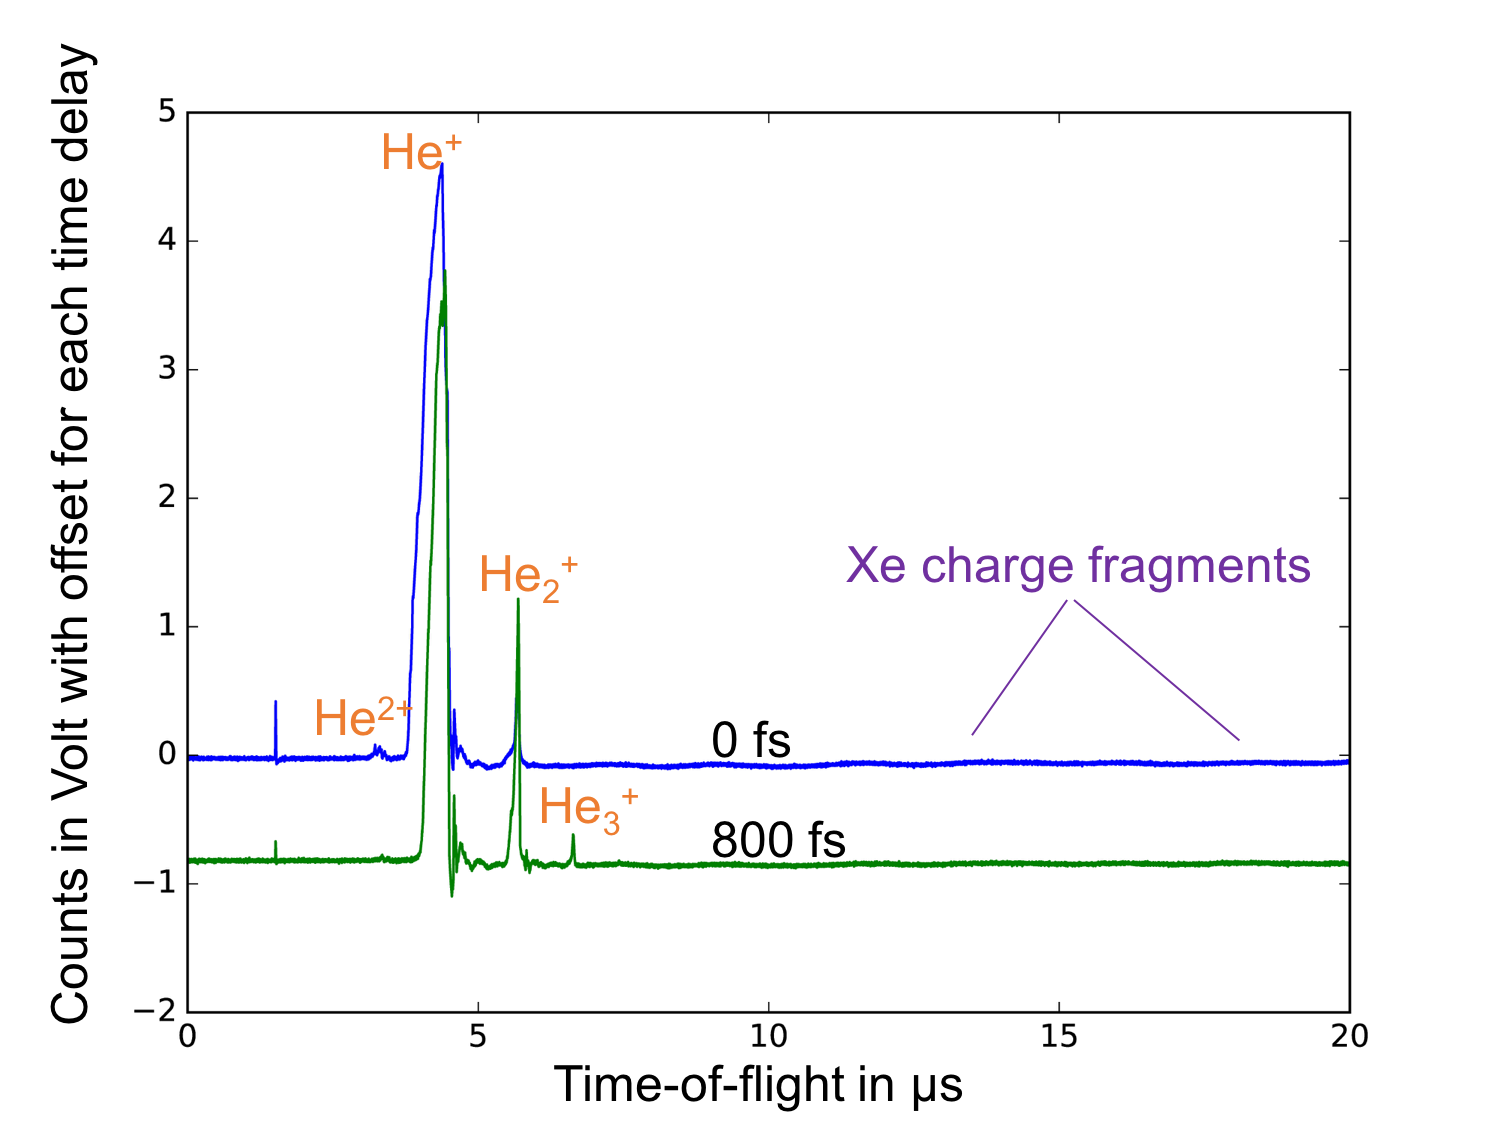
\includegraphics[width=0.65\textwidth]{images/results/TOF-helium-xenon-cluster-13-2.png}
 	\caption[TOF spectra of HeXe-clusters with \SI{\sim 0.06}{\percent} Xe-doping at various delays.]{Ion TOF spectra of HeXe-cluster with radius $r\approx$ \SI{775}{\nano\meter} and a \SI{\sim 0.06}{\percent} xenon doping level. These weaker doped HeXe-clusters show a lower He$^{2+}$-ion count and kinetic energy release. Barely any Xe-ions are detected.}
 	\label{fig:TOF-helium-xenon-cluster-13}
\end{figure}
%
If the He-ion composition is strongly driven by the doped Xe-atoms, one would expect a dependence on the Xe doping-level. Therefore, He-droplets with a radius of $r\approx$ \SI{775}{\nano\meter} and a \SI{\sim 0.06}{\percent} doping are discussed next. This is a \num{\sim 10} times less doping than the above discussed data and the He$^{2+}$-ion signal should therefore be less intense and broad to support the hypothesis. For completeness, the helium depletion is \SI{\sim 13}{\percent}. Figure \ref{fig:TOF-helium-xenon-cluster-13} shows the ion TOF data at delays $\Delta t=$ \SIlist{0;800}{\femto\second}. We note, again, the presence of $\text{He}^{2+}$ ions and an increased signal from $\text{He}^{+}$ ions. Although the He-droplet is larger, the $\text{He}^{2+}$-ion peak is clearly less intense and less broad than the above data with stronger Xe-doping. Xe-ions are barely detected. These data support the hypothesis that the Xe-particles drive the He-ionization through the above discussed processes. The detection of the initially photoionized xenon is more suppressed than in the above data through recombination effects and a larger electron reservoir. By varying the time delays $\Delta t$, the height of each He-ion peak shifts and a time-dependence is clearly visible. The $\text{He}^{2+}$ and $\text{He}^{+}$ states become less intense, but a stark increase in $\text{He}_{2}^{+}$ and $\text{He}_{3}^{+}$ peaks is observed. This could be a sign of a less violent nanoplasma expansion, where charge fragments not fully disintegrate into their atomic components, i.e., $\text{He}^{2+}$-ions, than in the above strongly doped data.\\[1\baselineskip]
%
%Summarizing, we studied the idea that a low-Z material acts as a sacrificial layer for the high-Z material using TOF mass spectroscopy. 
In summary, pristine He-droplets show little time-dependence as $\Delta t$ is varied and mostly singly-charged $\text{He}^{+}$- and $\text{He}_{2}^{+}$-ions are measured. If the He-droplets are doped with xenon, doubly-charged $\text{He}^{2+}$-ions are detected, the kinetic energy release is stronger, and the time-of-flight data reveal a He-ion time-dependence that is comparable to the one of Xe-atoms. As the Xe-doping is decreased, the presence of $\text{He}^{2+}$ ions becomes less frequent. This HeXe-cluster data indicates that the ionization dynamics of the He-ions are driven by the encapsulated Xe-atoms. A charge transfer from the initially photoionized Xe-atoms to the He-droplet is likely the dominating process leading to these TOF traces. This has also been shown previously theoretically \cite{Hau-Riege-2007-PRL} and in static studies \cite{Hoener-2008-JPB,Sugishima-2012-PRA,Muller-2015-JPhysB}. If the HeXe-cluster TOF data is compared to the pristine Xe-cluster TOF data, it becomes obvious that the Xe-particles preserve their integrity better when they are encapsulated in a He-cluster \cite{Hoener-2008-JPB,Muller-2015-JPhysB,Sugishima-2012-PRA}.
%This data could originate from an ultrafast and efficient kinetic energy transfer from the Xe-particles to the He-droplet. Collisions could drive this energy transfer. Charge-transfer ionization could drives the He-ion composition. Thereby, the He-droplet acts as an electron reservoir and the initially photoionized Xe-atoms recombine efficiently. Neutral xenon is not detected by the TOF mass spectrometer and this indicates that the Xe-particles in the HeXe-clusters preserve their integrity much better than pristine Xe-clusters. Pristine Xe-clusters are efficiently ionized and Xe-charge-fragments of Xe$^{25+}$ are observed, which indicate that the pristine Xe-cluster exhibit violent sample damage. Similar results have also been studied in \citep{Hoener-2008-JPB,Mikaberidze-2008-PRA}.
%
%
%
%%%%%%%%%%%%%%%%%%%%%%%%%%%%%%%%%%%%
%%%%%%%%%%%%%%%%%%%%%%%%%%%%%%%%%%%
%%%%%%%%%%%%%%%%%%%%%%%%%%%%%%%%%%%%
\section{Scattering response of rare-gas clusters}\label{sec:scattering-response}
%
%This section discusses the diffraction images that were obtained in the X-ray pump--X-ray probe study. The discussion begins with an assessment of the X-ray induced radiation damage of pristine Xe-clusters, whereby first diffraction images and then reconstructions are discussed, and an analysis of diffraction images of pristine He-droplets. This is followed by the discussion of the shape of HeXe-clusters. The section ends by discussing and comparing X-ray induced damage in HeXe-clusters to Xe- and He-clusters.
%
%
%
\subsection{Structural damage in Xe-clusters induced by intense X-rays}\label{sec:xenon-data}
%%%%%%%%%%%%%%%%%%%%%%%%%%%
%- Presentation of Xe data
%%%%%%%%%%%%%%%%%%%%%%%%%%%
% INTRO
XFELs can create high-quality diffraction images from single particles. All diffraction images carry transient information of the sample during the pulse \cite{Bostedt-2012-PRL}. In a pump-probe experiment, time-resolved structural information can be extracted from the diffraction images, such as the surface softening of the nanoplasma \cite{Gorkhover-2016-NatPho}. This thesis experiment follows the X-ray induced nanoplasma expansion up to \SI{800}{\femto\second} for the first time.
%A very distinct time-resolved signal originates from the surface softening of the clusters as they undergo the nanoplasma expansion \cite{Gorkhover-2016-NatPho}. To investigate this time-dependent signal, 
To start out, \numrange{30}{60} diffraction images per delay step from Xe-clusters are analyzed (see Section \ref{sec:hitfinding}) and their radius is determined. This leads to a high-throughput evaluation of several hundred clusters, whereby Equation \eqref{eq:scattering from sphere} is exploited to automatically fit diffraction images.\\[1\baselineskip]
% SIZE EFFECTS
\begin{figure}
	\centering
		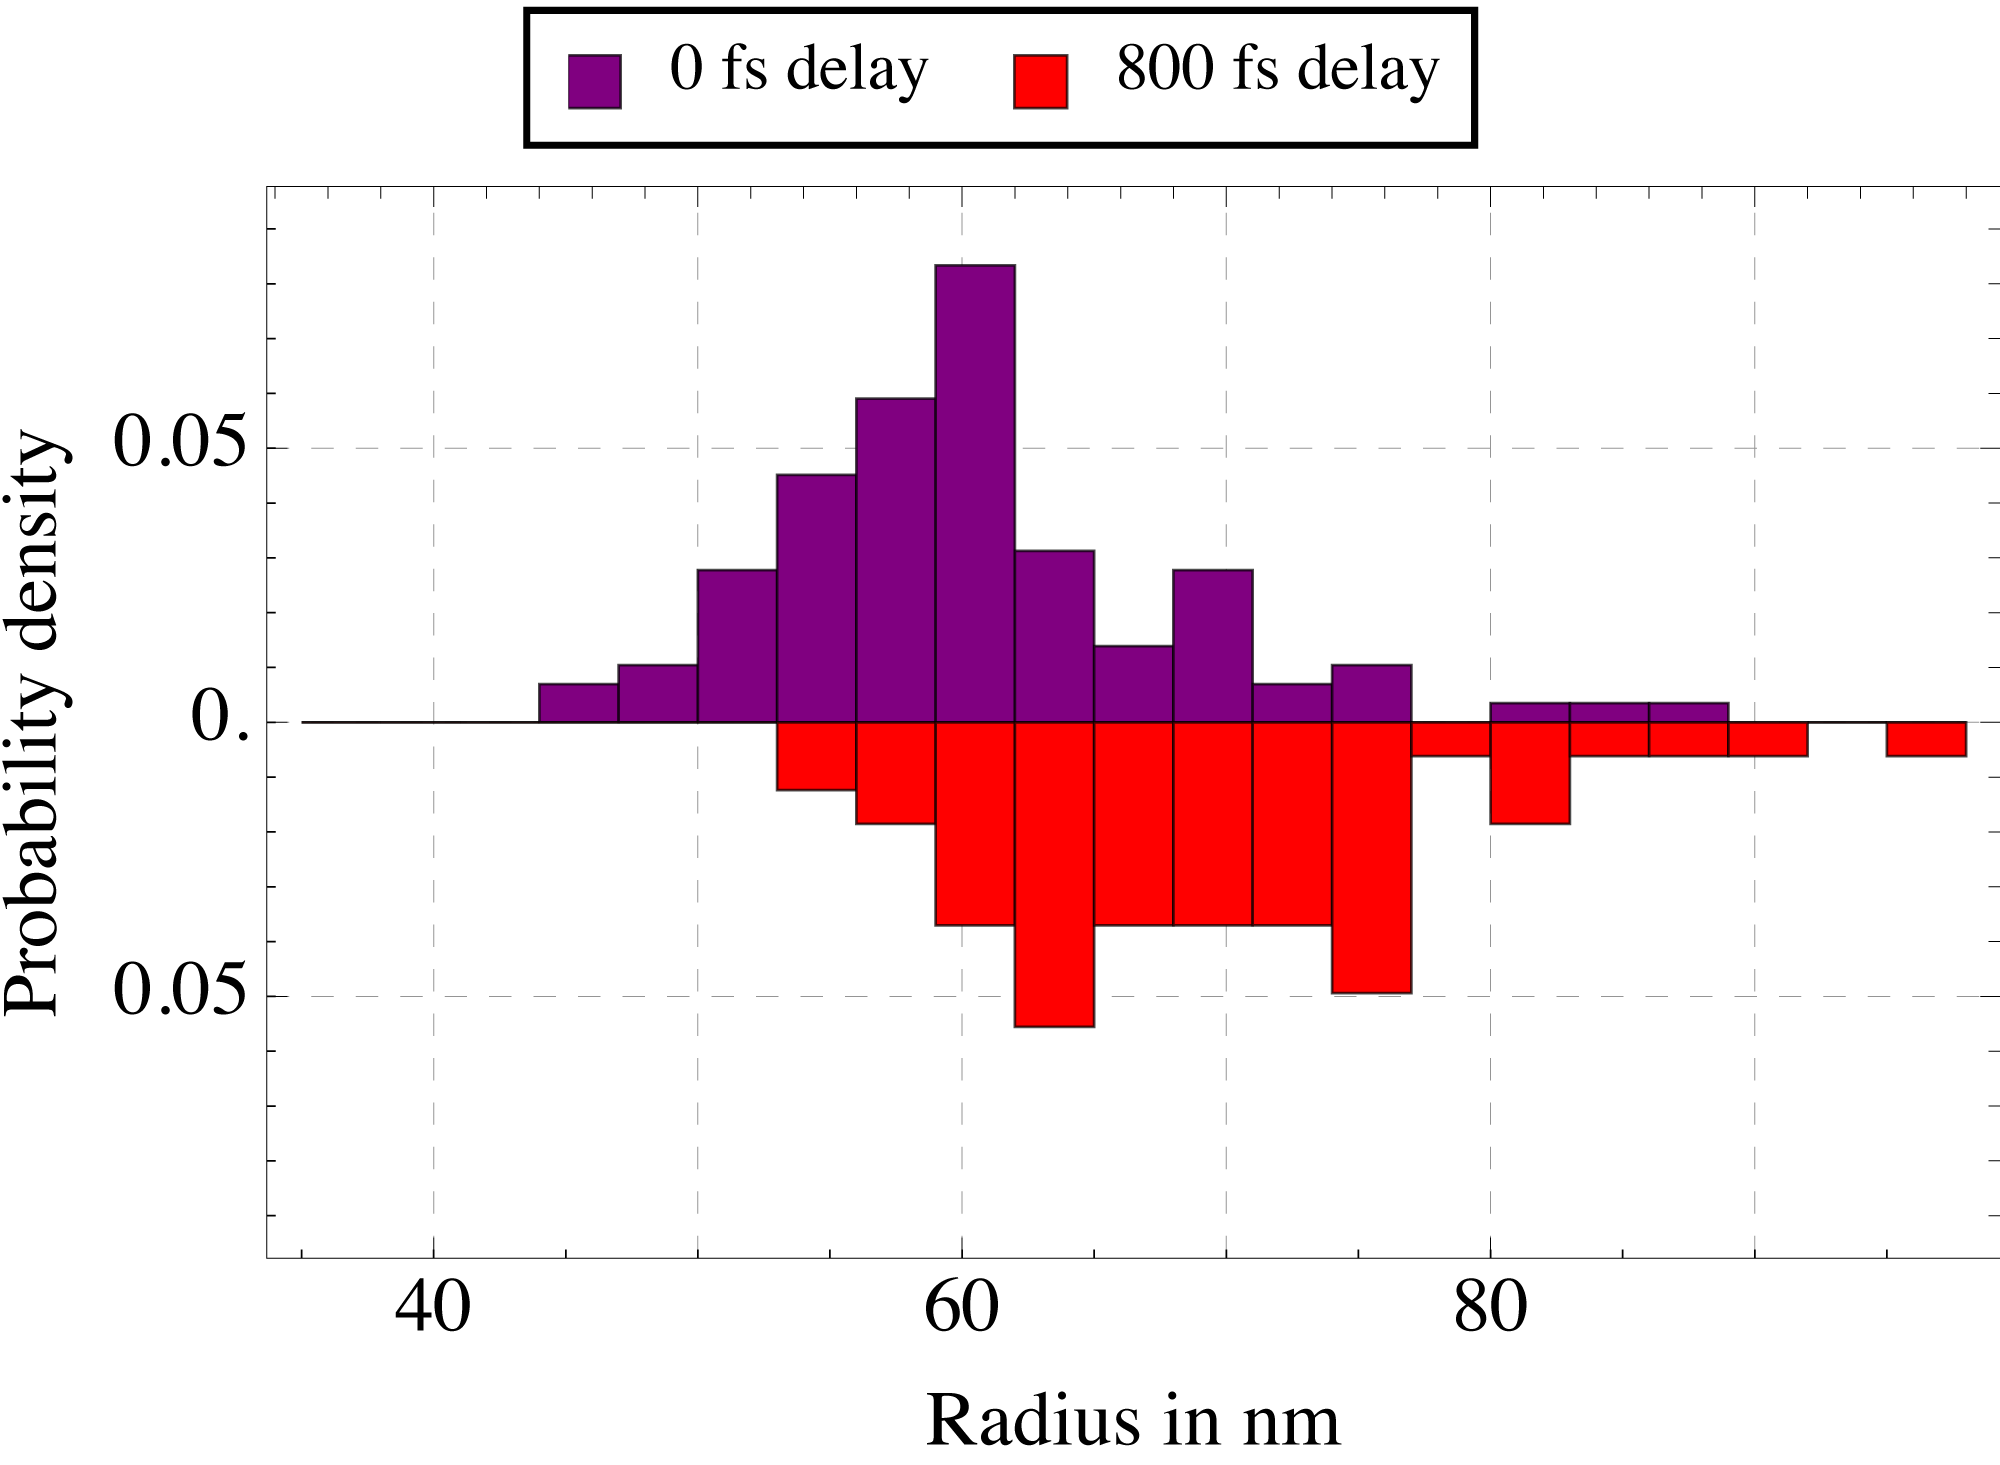
\includegraphics[width=0.70\textwidth]{images/results/size-distributions.png}
	\caption[Single Xe-cluster size distribution at varying time delay $\Delta t$.]{Size evaluation of \num{\sim 30} single Xe-cluster hits per time delay $\Delta t$ step. At $\Delta t=\SI{0}{\femto\second}$, the size distribution follows in approximation an expected log-normal distribution. At $\Delta t=\SI{800}{\femto\second}$ the distribution broadens and shifts towards larger radii due to the nanoplasma transition.}
	\label{fig:size-distributions}
\end{figure}
Supersonic gas jets always produce a distribution of cluster sizes (see Section \ref{sec:homogenous-cluster}). Such a distribution of cluster radii is shown in Figure \ref{fig:size-distributions} for the X-ray pump--X-ray probe time delays, $\Delta t =$ \SIlist{0;800}{\femto\second}. The size distribution of Xe-clusters follows a log-normal distribution \citep{Schutte-2002-IJMS} and for $\Delta t=0$ fs, the mean cluster radius is \SI{61}{\nano\meter}. When the imaging pulse is delayed by $\Delta t=$ \SI{800}{\femto\second}, the mean cluster-radius increases to \SI{74}{\nano\meter} and the size-distribution becomes broad. This can be clearly attributed to the nanoplasma expansion. The Xe-cluster size distribution may become more broad due to a distribution of the pump-pulse power density. Shot-to-shot fluctuations result in different nanoplasma expansion speeds, $v_{\text{exp}}$, as discussed below.\\[1\baselineskip]
%
\begin{figure}
	\centering
		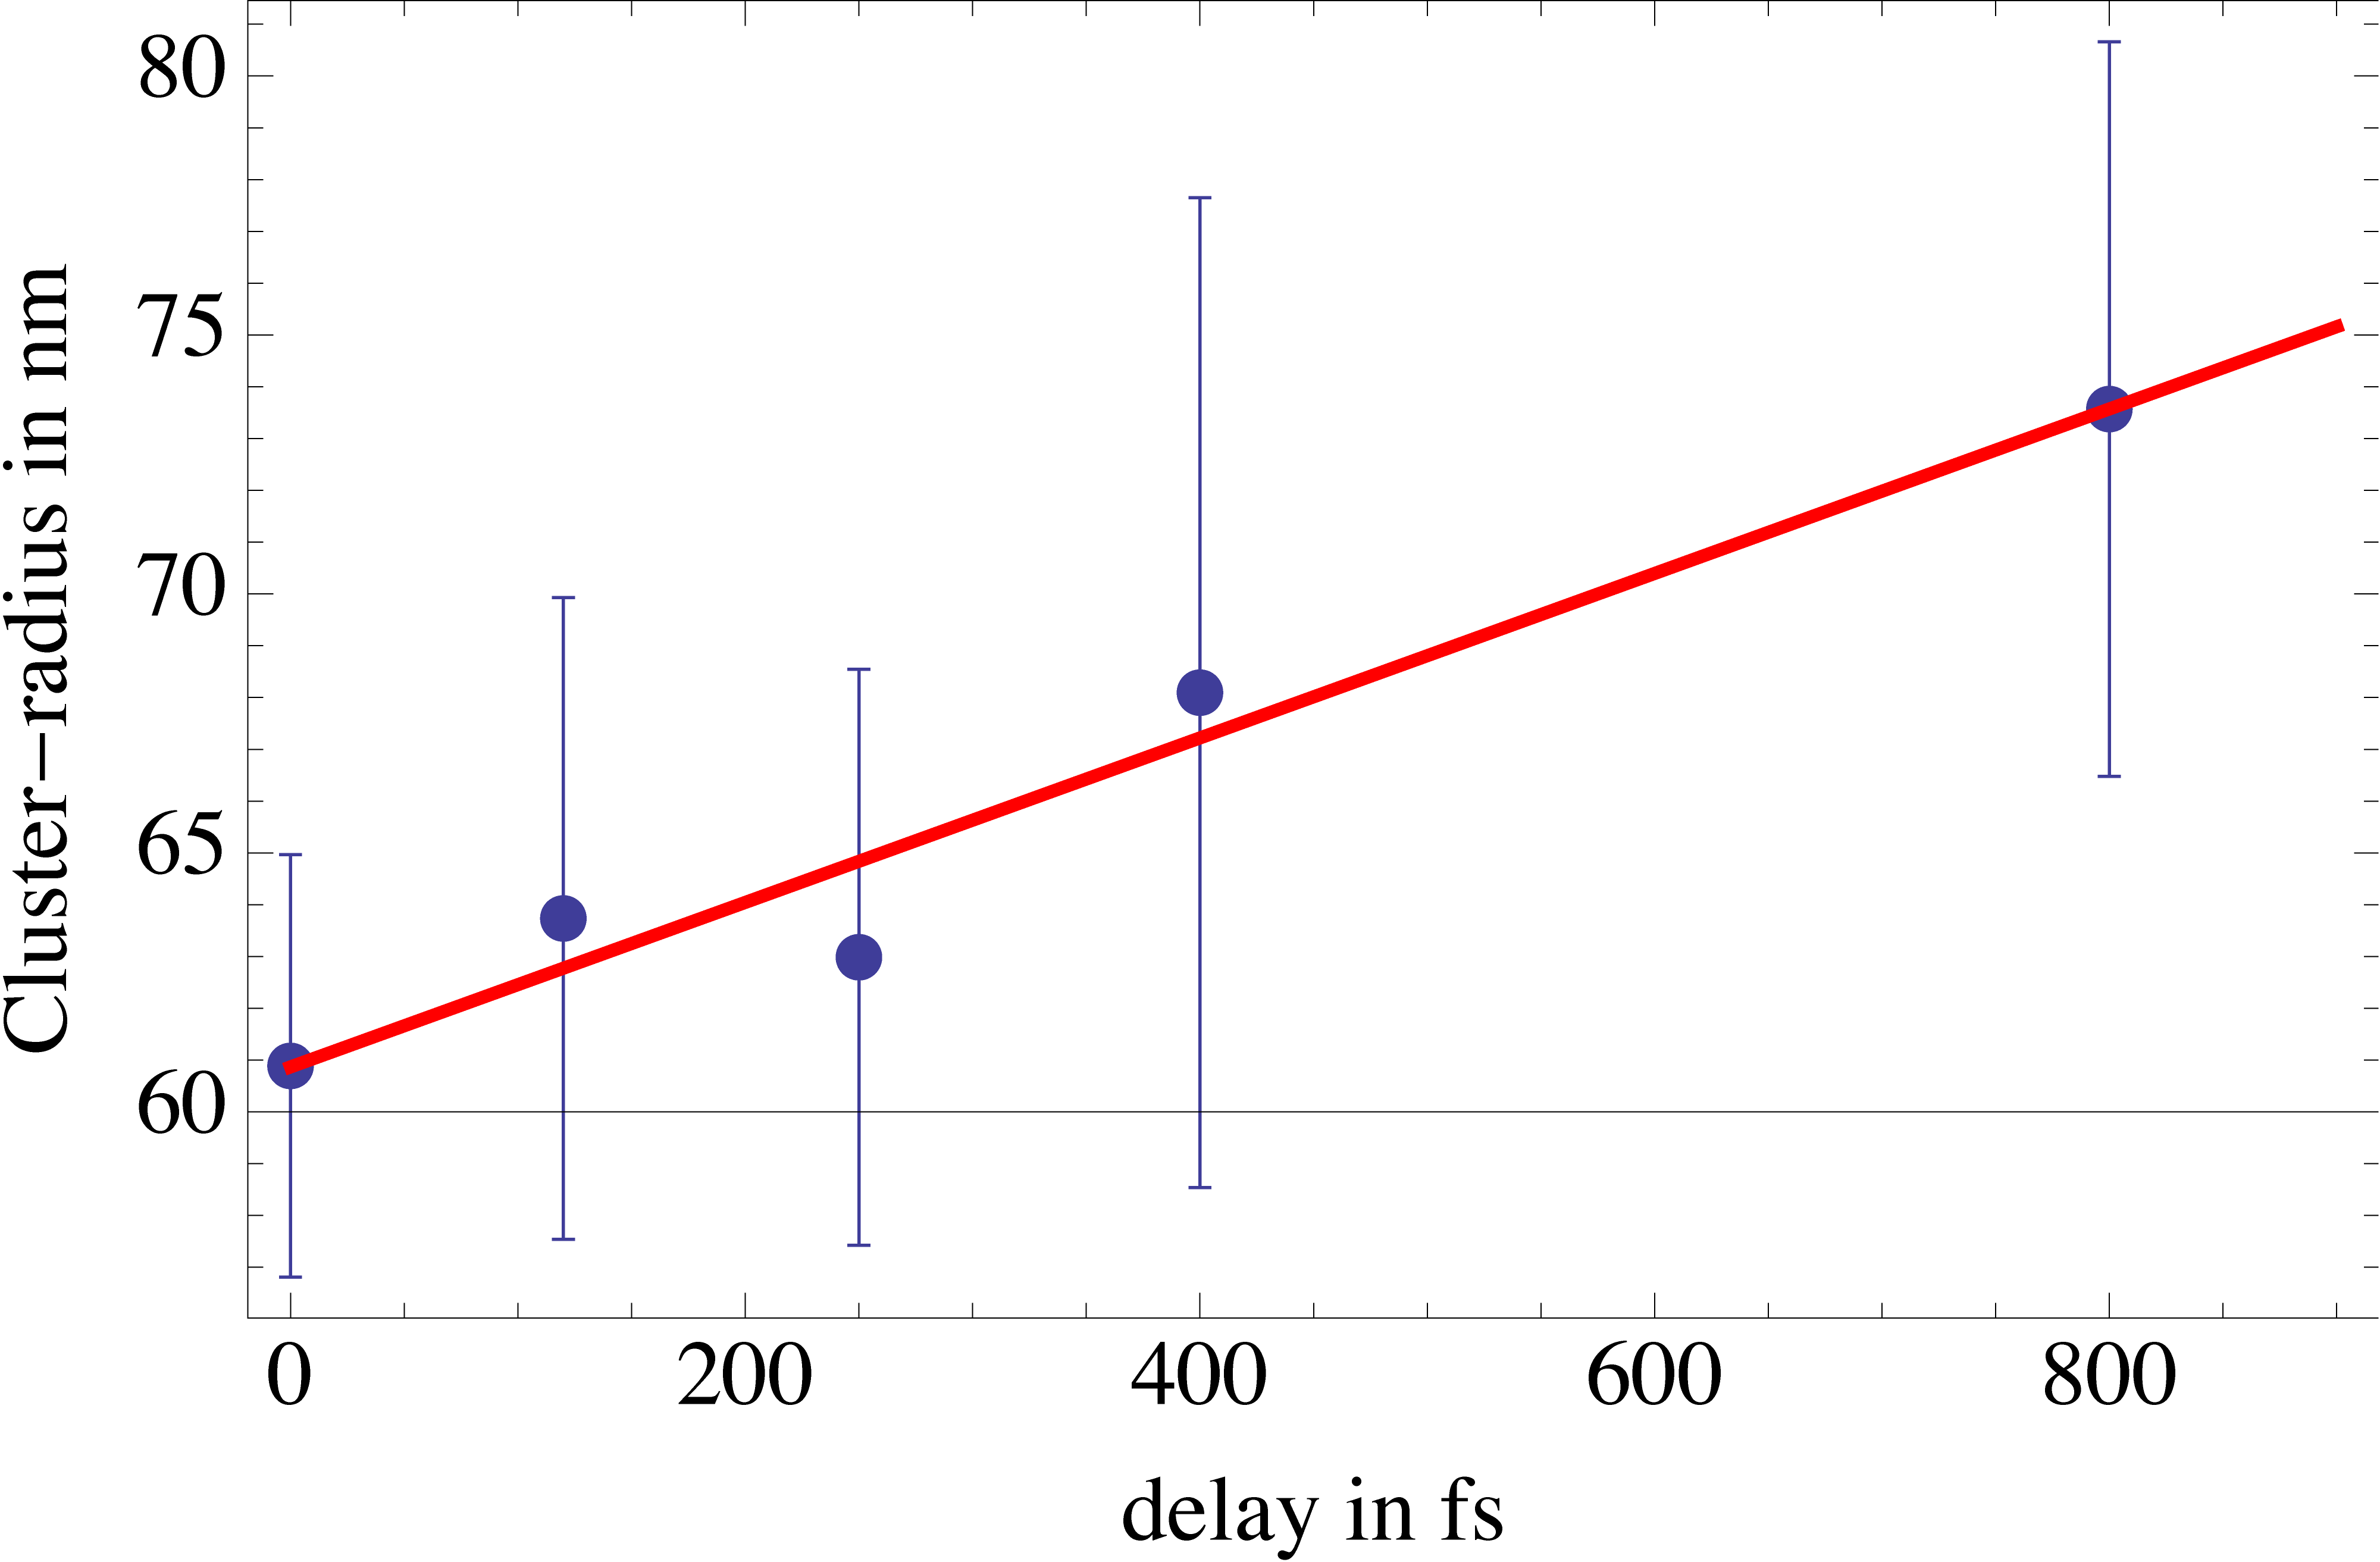
\includegraphics[width=0.49\textwidth]{images/results/filter-size.png}
		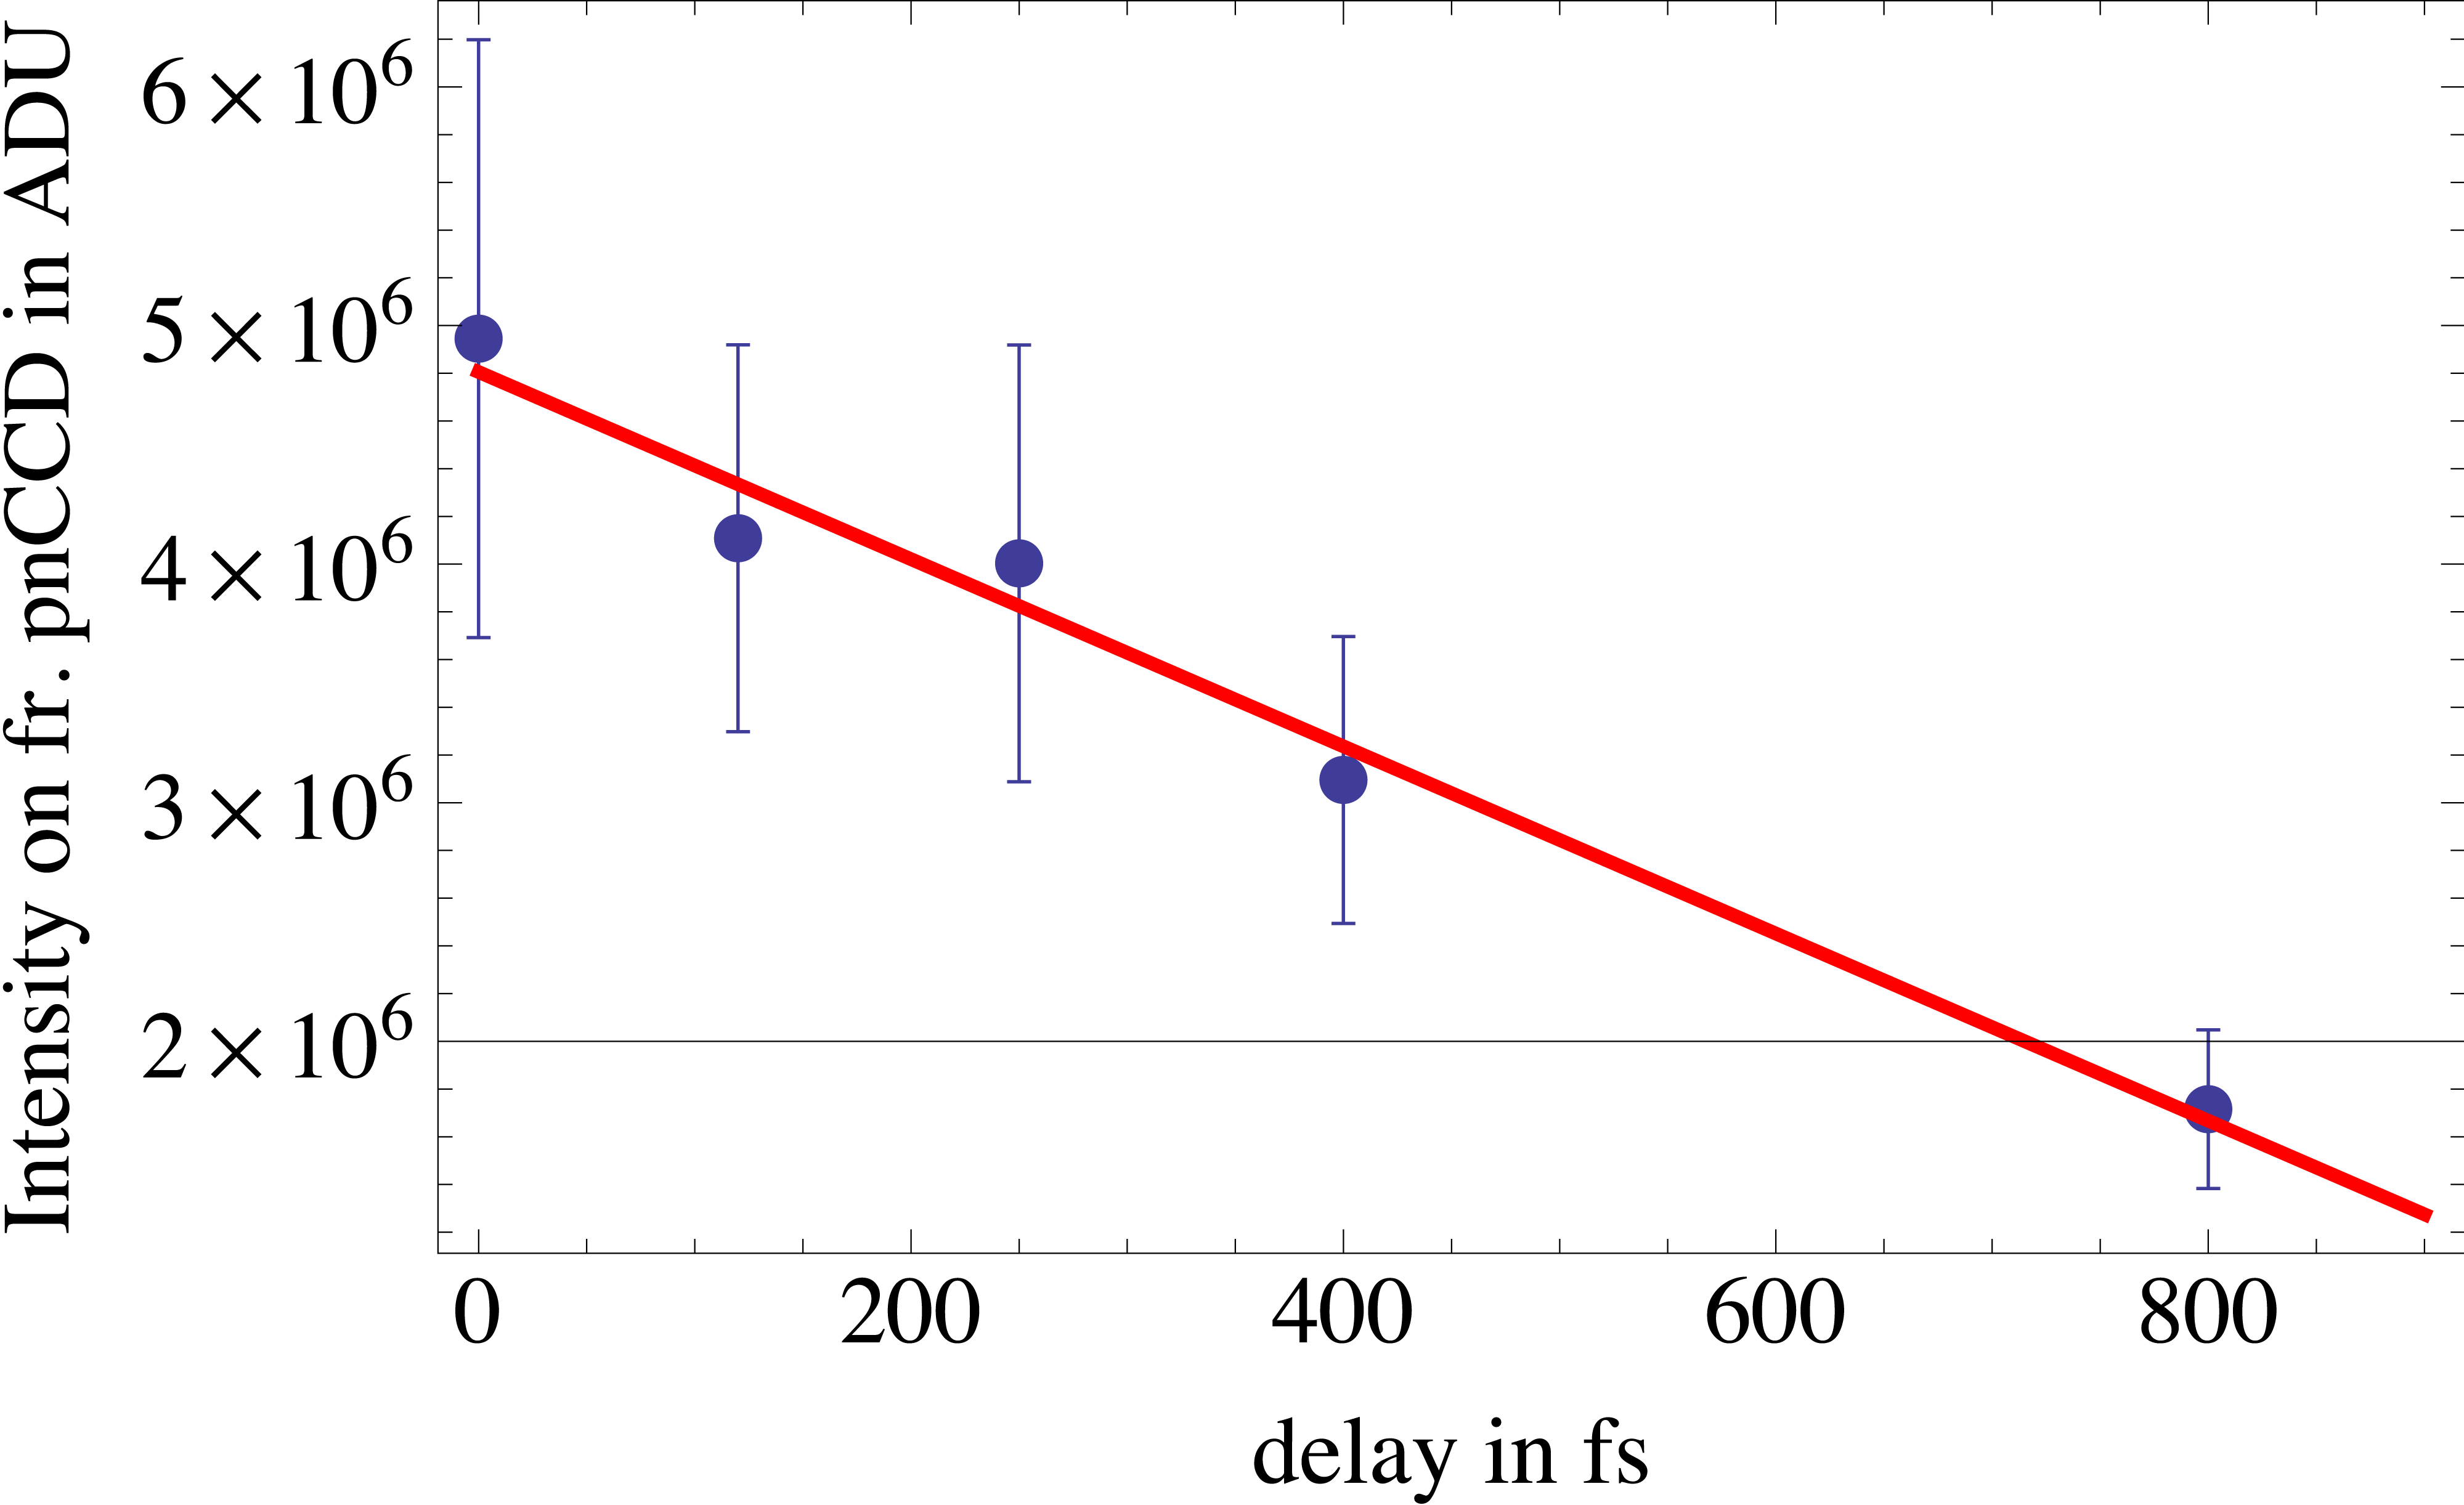
\includegraphics[width=0.50\textwidth]{images/results/filter-sum-frontpnCCD.png}
	\caption[Average cluster size correlated to measured intensity on front pnCCD.]{Average xenon cluster size of intense hits as a function of pump--probe delay $\Delta t$ (left panel). Average intensity on the front pnCCD of intense single-shot hits from single Xe-cluster as a function of the pump--probe delay $\Delta t$ (right panel).}
	\label{fig:filter-size-intensity}
\end{figure}
%
A summary of the of the Xe-cluster radii increase over several pump--probe delay steps can be found in Figure \ref{fig:filter-size-intensity}. The mean radii and standard deviations of the log-normal distributions are plotted for $\Delta t=$ \SIlist{0;120;250;400;800}{\femto\second} and fitted linearly. These data suggest that the nanoplasma expansion speed, $v_{\text{exp}}$, is rather constant over the observation window. Theoretical studies of nanoparticles \cite{Hau-Riege-2004-PRE,Mikaberidze-2008-PRA,Ho-2016-PRA} predict that the expansion speed indeed becomes constant after a few ten femtoseconds, which the system needs to thermalize. We can determine the expansion speed using the mean increase of cluster-radii over $\Delta t=$ \SIlist{0;800}{\femto\second} and note $v_{\text{exp}}\approx \SI{15250}{\meter\per\second}$. This indicates that Xe-nanoparticles that are irradiated with typical LCLS pulses undergo a violent and rapid explosion.\\[1\baselineskip]
%
We can use the expansion speed to estimate the electron temperature of the nanoplasma, as it has been done similarly before \cite{Gorkhover-2012-PRL}. Thereby, we should note that the electron gas of the nanoplasma thermalizes with the ions on the few femtoseconds time-scale and follows a Maxwell-Boltzmann distribution \cite{Arbeiter-2011-NJP}. If we now find a temperature for the Maxwell-Boltzmann distribution that has the expansion speed, $v_{\text{exp}}$, as mean velocity, we can estimate the electron temperature to be \SI{\sim 125}{\electronvolt}. This compares to temperatures that can be found inside the sun.\\[1\baselineskip]
%
We can also compare the electron temperature to a similar NIR pump--X-ray probe nanoplasma study on Xe-clusters \cite{Gorkhover-2016-NatPho}, where electron temperatures of \SI{\sim 200}{\electronvolt} have been found. The difference in electron temperature and expansion speed is attributed to the difference between the NIR and X-ray pump-pulse parameters and the corresponding absorption cross-sections. The NIR pump-pulse has a wavelength of \SI{800}{\nano\meter}, a focal spot size of \SI{1600}{\micro\meter\squared}, and power densities of \SI{\sim e15}{\watt\per\square\centi\meter} \cite{Gorkhover-2016-NatPho}. The X-ray pump-pulse in this study has a wavelength of \SI{1.5}{\nano\meter} and power densities of \SI{\sim 2e16}{\watt\per\square\centi\meter}. The NIR strong-field absorption cross-section of a xenon atom can be estimated to be \SI{\sim 30}{\mega\barn} using the above power densities (from Reference \cite[][1826]{Fennel-2010-RMP}), and the X-ray absorption cross-section for atomic xenon is \SI{\sim 3}{\mega\barn} (from Figure \ref{fig:photoionization}). Let us perform a very simplified cross-section estimation similar to Equation \eqref{eq:absorption-cross-section} using \SI{25}{\nano\meter} radius Xe-clusters. Given the above parameters, this estimation indicates that a Xe-cluster would absorb \SI{\sim 93}{\kilo\electronvolt} in the NIR and \SI{\sim 79}{\kilo\electronvolt} in the X-ray wavelength region. The relative absorbed energy in X-ray versus NIR is $\tfrac{79}{93}\si[per-mode = fraction]{\cancel\kilo\electronvolt\per\cancel\kilo\electronvolt}\approx\SI{85}{\percent}$. This relative difference can be compared to the relative difference in electron temperatures of the X-ray-- vs. the NIR--study, which is $\tfrac{125}{200}\si[per-mode = fraction]{\cancel\electronvolt\per\cancel\electronvolt}\approx\SI{63}{\percent}$. Given this estimate, it is clear why the electron temperature in the NIR study is higher than in the here presented X-ray study. It is noted that, for example, transient scattering factors and cluster cooling processes \cite{Fennel-2010-RMP} do play a significant role in this absorption process, which do vary the actual absorbed energies drastically \cite{Fennel-2010-RMP} and are disregarded in this simplified estimate.\\[1\baselineskip]
%X-ray absorption cross-section of xenon, $\sigma_{\text{X-ray}}=\SI{\sim 3}{\mega\barn}$ is much smaller than the IR cross-section, $\sigma_{\text{IR}}=\SI{\sim 30}{\mega\barn}$. Ultimately, the Xe-clusters absorb more energy from IR pump-pulses than X-ray pump-pulses of similar power density.\\[1\baselineskip]
% NO OF SCATTERER
\begin{figure}
	\centering
		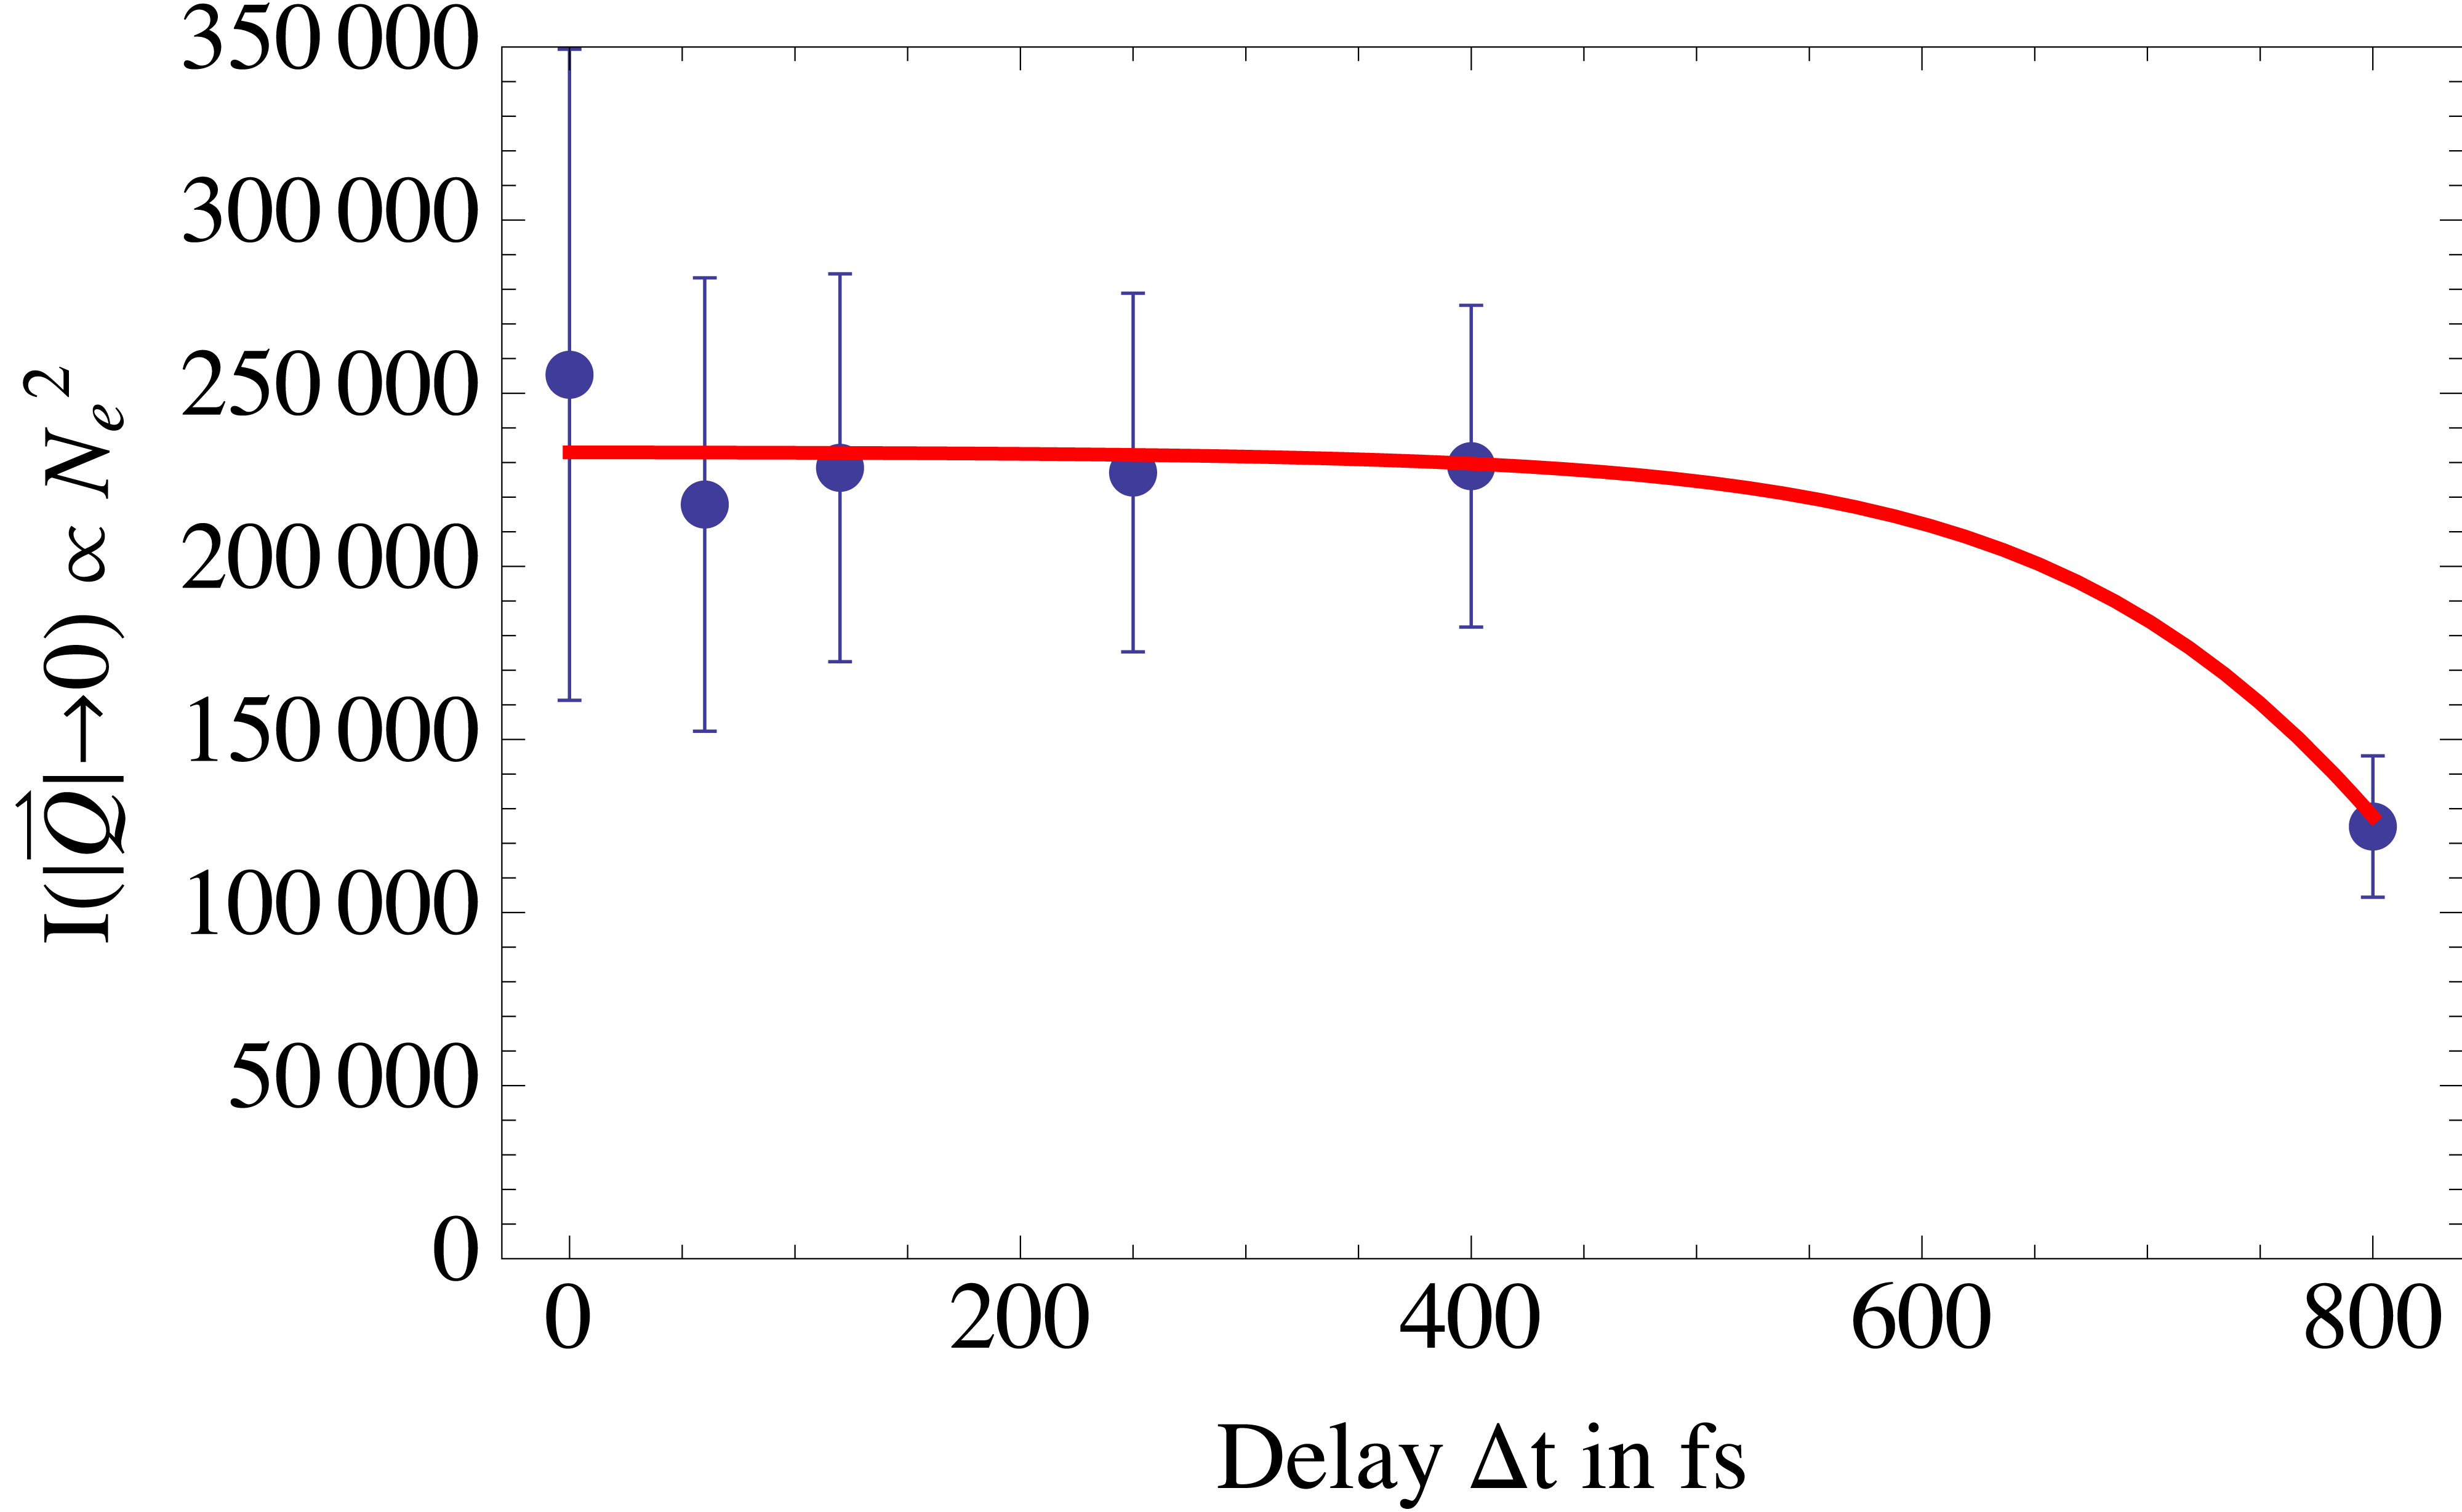
\includegraphics[width=0.80\textwidth]{images/results/number-of-scatterers.png}
	\caption[Time-resolved behavior of number of scatterers due to nanoplasma expansion]{Scattered intensity $I_{0}$ in arb. units at $\vec{Q}\rightarrow 0$ of Xe-clusters. This is proportional to the total number of scatterers squared, $N_{e}^{2}$. The red curve is a guide for the eye (see Section \ref{sec:xenon-data}).}
	\label{fig:number-of-scatterer}
\end{figure}
%
Let us continue by looking at the time-dependent behavior of electrons. During the pulse the cluster is increasingly ionized, the Coulomb potential deepens, and eventually electrons from photoionization processes are efficiently trapped \cite{Arbeiter-2011-NJP}. On a larger timescale, the cluster or now nanoplasma expands, the Coulomb potential lowers again, and the thermalized electrons can escape the potential (see Section \ref{sec:nanoplasma-expansion}). The diffraction images carry, in principle, information about the total number of coherent scatterers and we can therefore estimate the number of electrons in the cluster over $\Delta t$. The single-shot diffraction pattern analysis from above also determines the intensity of the forward scattering (see Section \ref{sec:saxs}), which is proportional to
%The total number of scatterers, i.e., electrons that interact with the LCLS pump-pulse, is deduced from the diffraction patterns via an intensity analysis. As described in the theory Section \ref{sec:saxs}, when
\begin{equation}{}
I\left(\vec{Q}\rightarrow 0\right) \propto N_{e}^{2},
\label{eq:intensity-prop-to-electrons}
\end{equation}
where $I$ is the distribution of the scattered intensity as a function of the scattering vector $\vec{Q}$, and $N_{e}$ is approximately the number of electrons - as discussed in Section \ref{sec:saxs}. We also assume that the coherent forward-scattering of the most intense LCLS hits is comparable on a shot-to-shot basis \cite{Gorkhover-2012-PRL}. Using Equation \eqref{eq:scattering from sphere}, Figure \ref{fig:number-of-scatterer} shows the intensity $I\left(\vec{Q}\rightarrow 0\right)$ as a function of the time delay, $\Delta t$ (blue dots).
%As the incident beam intensity, $I_{0}$, remains constant in the X-ray pump--X-ray probe setup $\rho_{0}^{2} \propto N_{e}^{2}$. Two linear fits (red lines) have been added to the figure to visualize the effect.
%The data show that up to a delay of $\Delta t\approx$ \SI{400}{\femto\second} the amount of electrons $N_{e}$ in the interaction region rather constant.
Even considering the large error bars that originate from the standard deviation of the intensity distribution from the single-shot diffraction images, the data show a more rapid evaporation of electrons between \SIrange{400}{800}{\femto\second} than between \SIrange{0}{400}{\femto\second}. For the total time delay range of $\Delta t=$ \SIrange{0}{800}{\femto\second}, the number of scattering electrons decreases on average by \SI{\sim 26}{\percent} (see Figure \ref{fig:number-of-scatterer}), while the Xe-clusters increase in radius by \SI{\sim 20}{\percent} (see Figure \ref{fig:filter-size-intensity}). In a simple electro-static model \cite{Arbeiter-2010-PRA,Ditmire-1996-PRA}, the potential of the plasma can be described by a homogeneously charged and expanding sphere. The kinetic energy of electrons that are trapped in this potential may be described using a Maxwell-Boltzmann distribution. In this case, the trapped electrons can escape the cluster potential depending on their kinetic energy and the potential depth. The hypothesis is that electrons are efficiently trapped at first, but the expansion of the cluster lowers the potential allowing the trapped electrons to escape. With the in this study measured cluster sizes and expansion speeds, this simplified model cannot reproduce the data points of Figure \ref{fig:number-of-scatterer}. Using the above stated expansion speed, electron temperature, and cluster-size, this simplified model indicates no loss of electrons in the given time window of \SI{800}{\femto\second}. In order for this model to fit the data, \num{\sim10} times larger expansion speeds, $v_{\text{exp}}$, would have to be used (see red line in Figure \ref{fig:number-of-scatterer}). This could be a signature of anisotropic effects in the nanoplasma expansion \cite{Peltz-2014-PRL,Mikaberidze-2009-PRL}. More data, particularly at longer time delays, would be needed to develop an accurate model.\\[1\baselineskip]
%As the electrons follow the Maxwell-Boltzmann distribution including the typical \text{tail}, some few electrons have large kinetic energies and should be able to overcome the Coulomb barrier in the initial stages of the nanoplasma expansion. As the Coulomb barrier decreases, more and more electrons have enough kinetic energy to overcome the trapping potential.
%
%This supports the idea that the Coulomb barrier\index{nanoplasma expansion!Coulomb trapping} efficiently traps electrons in the initial stages of the nanoplasma expansion\index{nanoplasma!expansion}. But as the nanoplasma expansion progresses, the electrons overcome the trapping potential and are ejected. The key driver that lowers the trapping potential, thus releasing the electrons, is the expansion of the cluster. The effect of trapped electrons in a nanoplasma have been simulated in, e.g., \citep{Hau-Riege-2004-PRE}. Trapped electrons contribute drastically to the sample damage due to secondary collisional ionization.
The scattering and TOF data so far indicate that Coulomb trapped electrons may play a significant role in the nanoplasma. Trapped electrons damage the sample via secondary collisional ionization \cite{Hau-Riege-2004-PRE}. The key driver releasing trapped electrons is the nanoplasma expansion that lowers the Coulomb potential \cite{Arbeiter-2011-NJP}. It should be noted that trapped electrons also contribute to the diffraction image. In a thought-experiment, where a single-particle imaging (SPI) experiment is performed using comparably long X-ray pulses of \SI{\sim 100}{\femto\second}, trapped electrons can be treated non-relativistic such that they contribute coherently to the diffraction image \cite{Williams-2016-PC}. The delocalization of the trapped electrons and the widening of the cluster potential well reduce the contrast of diffraction images. This kind of radiation damage occurs on the timescale of Coulomb trapping and Figure \ref{fig:number-of-scatterer} indicates that the Coulomb trapping is efficient upon the first time-resolved data points with delays comparable to the pulse length in this thought experiment. Therefore, \SI{\sim 100}{\femto\second} long pulses - as they are sometimes used at LCLS to perform SPI experiments - carry information of trapped electrons. This is a form of radiation damage and is described in Reference \citep{Quiney-2010-NatPhys}. In this Reference, computational methods are presented and predicted to compensate for such damage.\\[1\baselineskip]
%
%In a thought-experiment, where a SPI experiment is performed using long X-ray pulses of \num{\sim 100} fs, the sample would get ionized and efficiently traps electrons. The trapped electrons can be treated as non-relativistic, 
%But, trapped electrons also contribute to the scattering pattern. In a diffractive imaging experiment with long pulse durations of \SI{\sim100}{\femto\second}, the trapped electrons can be treated as non-relativistic such that they do contribute coherently to the scattering pattern \cite{Williams-2016-PC}.
%In a thought-experiment, where diffractive imaging is performed using X-ray pulses  pulse durationHowever, their contributions reduce the contrast of the diffraction image as they are delocalized. 
%
%
%
% SINGLE SHOT DIFF PATTERN
\begin{figure}
	\centering
		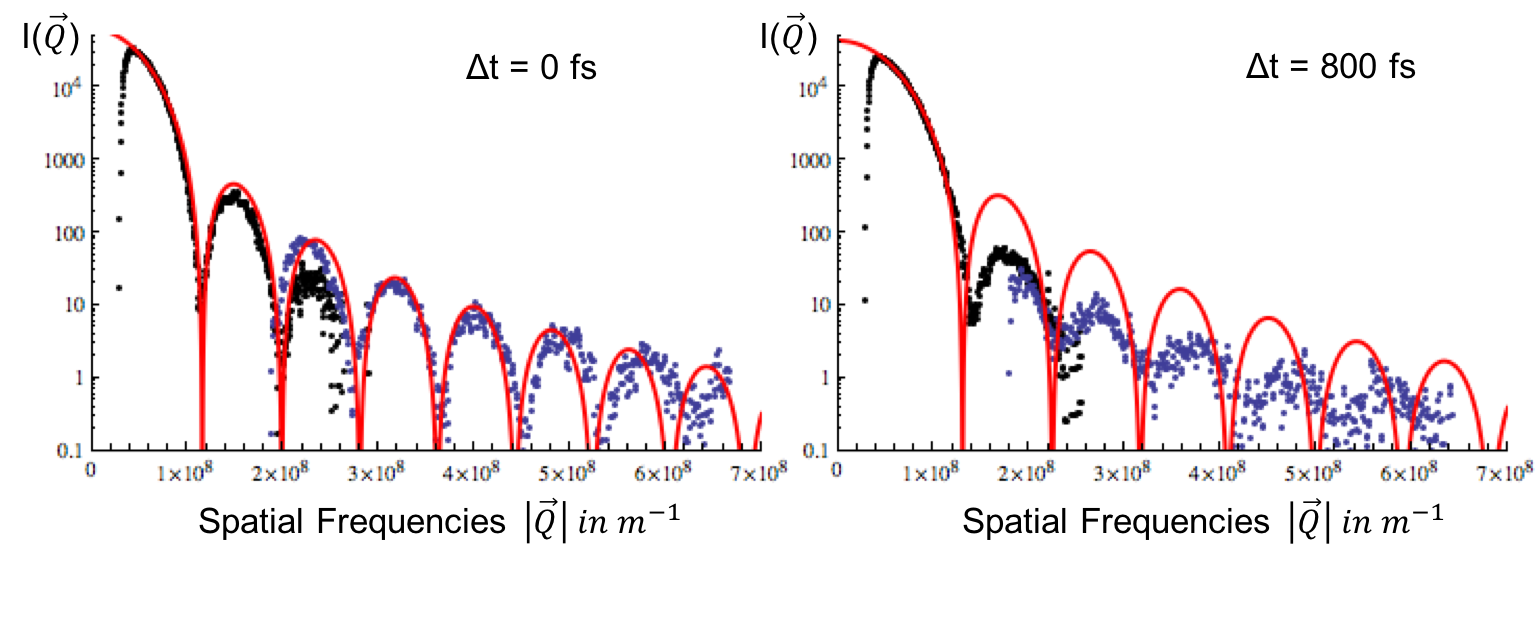
\includegraphics[width=1.0\textwidth]{images/results/Xe-diff-pattern.png}
		%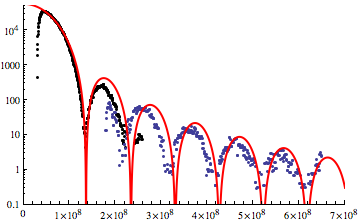
\includegraphics[width=0.49\textwidth]{images/results/Xe-only-60fs.png}\\
		%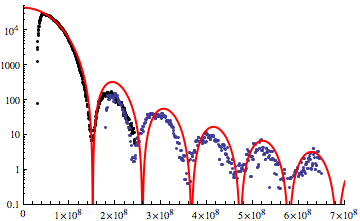
\includegraphics[width=0.49\textwidth]{images/results/Xe-only-120fs.png}
		%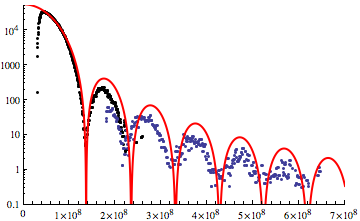
\includegraphics[width=0.49\textwidth]{images/results/Xe-only-250fs.png}\\
		%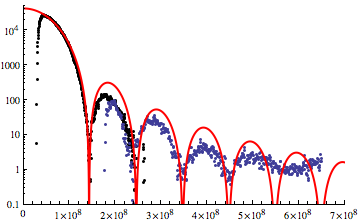
\includegraphics[width=0.49\textwidth]{images/results/Xe-only-400fs.png}
		%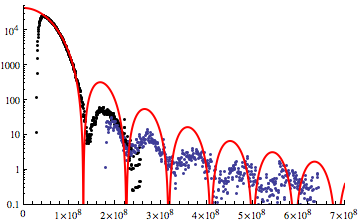
\includegraphics[width=0.49\textwidth]{images/results/Xe-only-800fs.png}
	\caption[Single-shot diffraction patterns of Xe-clusters at varying time delays]{Single-shot diffraction patterns of single Xe-clusters at certain pump--probe delays $\Delta t$. The red curve simulates the scattering of a sphere, the black data points are from the rear pnCCD detector and the blue data points are from the front pnCCD. The nanoplasma expansion manifests in the scattering intensity $I$ at high spatial-frequencies $\lvert \vec{Q}\rvert$, where $I$ decreases as described in \citep{Gorkhover-2016-NatPho}.}
	\label{fig:Xe-only-diff-pattern}
\end{figure}
We may also analyze the Xe-clusters on a shot-to-shot basis. Similar to previous studies \cite{Gorkhover-2016-NatPho,Rupp-2016-Springer,Bostedt-2012-PRL} radial projections of the measured diffraction patterns reveal structural information of the nanoplasma. In particular an optical pump--X-ray probe study on Xe-clusters \cite{Gorkhover-2016-NatPho} revealed that Xe-clusters exhibit a surface softening.
%Especially the investigation \cite{Gorkhover-2016-NatPho}, which was an IR pump--X-ray probe study investigating Xe-cluster, revealed that Xe-cluster exhibit a surface-softening by analyzing single diffraction patterns. 
Here, an electron density model similar to the one described in Section \ref{sec:2d-simulations} was established and the model was fitted to the diffraction pattern. The surface expansion thereby manifested in the diffraction pattern as a decline of the scattering intensity distribution at higher spatial frequencies. The analysis from above already indicated this in the right panel Figure \ref{fig:filter-size-intensity}, where the average scattering intensity on the front pnCCD detector was measured as a function of $\Delta t$. To show similarities to this optical pump--X-ray probe study, radial projections of single-shot diffraction patterns from single Xe-clusters are shown in Figure \ref{fig:Xe-only-diff-pattern}. The figure shows a red line, which is the scattering from a sphere as per Equation \eqref{eq:scattered-intensity} and \eqref{eq:scattering from sphere} fitted onto the low-$\lvert\vec{Q}\rvert$ signal of the zeroth diffraction scattering order using the radius and the incident beam intensity variables. The black data points are projected from the rear pnCCD and the blue data points are projected from the front pnCCD using the projection method described in Section \ref{sec:combination-of-images}. For $\Delta t=$ \SI{0}{\femto\second}, the scattering of the Xe-cluster can be well approximated with the scattering of a sphere. The ``spherical fit'' (red line) agrees well with the data points up to scattering angles of $\Theta \approx$ \SI{9}{\degree} or $\lvert\vec{Q}\rvert\approx\SI{6.8e8}{\per\meter}$. However, it should be noted that this comparison becomes less good at very large scattering angles due to deviations of the cluster from a perfect sphere. Above scattering angles of \SI{\sim 10}{\degree}, the flat detector surface should be accounted for \citep{Bostedt-2012-PRL}, but it plays a negligible role in this thesis experiment. As the time delay $\Delta t$ increases, the large-$\lvert\vec{Q}\rvert$ scattering signal decreases and the scattering of a plain sphere does not fit the scattering well anymore. The surface softening model from Section \ref{sec:2d-simulations} generally fits the data well, which indicates that an X-ray induced nanoplasma is also undergoing a surface softening comparably to previous studies \cite{Gorkhover-2016-NatPho,Gorkhover-2014-Thesis}. Note that the X-ray pump--X-ray probe considerations from Section \ref{sec:pump--probe-considerations} would minimize the effect of a decreased scattering at large scattering angles.\\[1\baselineskip]
%
%
%A similar effect is also observed in the previously mentioned IR pump--X-ray probe study \citep{Gorkhover-2016-NatPho}. 
%Due to the nanoplasma transition, the Xe-cluster is expanding with the outer layers expanding faster than the core. A mathematical description of this damage model, namely an expanding sphere, has been introduced in Section \ref{sec:2d-simulations}. 
%It generally fits the data well, as it is shown in great detail in \citep{Gorkhover-2016-NatPho,Gorkhover-2014-Thesis}. Note that the X-ray pump--X-ray probe considerations from Section \ref{sec:pump--probe-considerations} would minimize the effect of a decreased scattering at large scattering angles.
%
%
%
% 2D RECONSTRUCTIONS
\begin{figure}
	\centering
		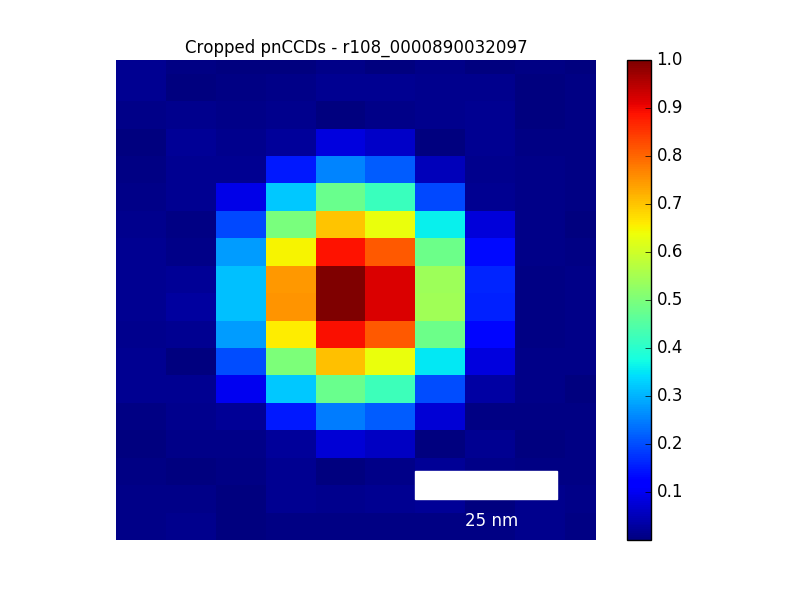
\includegraphics[width=0.46\textwidth]{images/results/Xe_0_fs.png}
		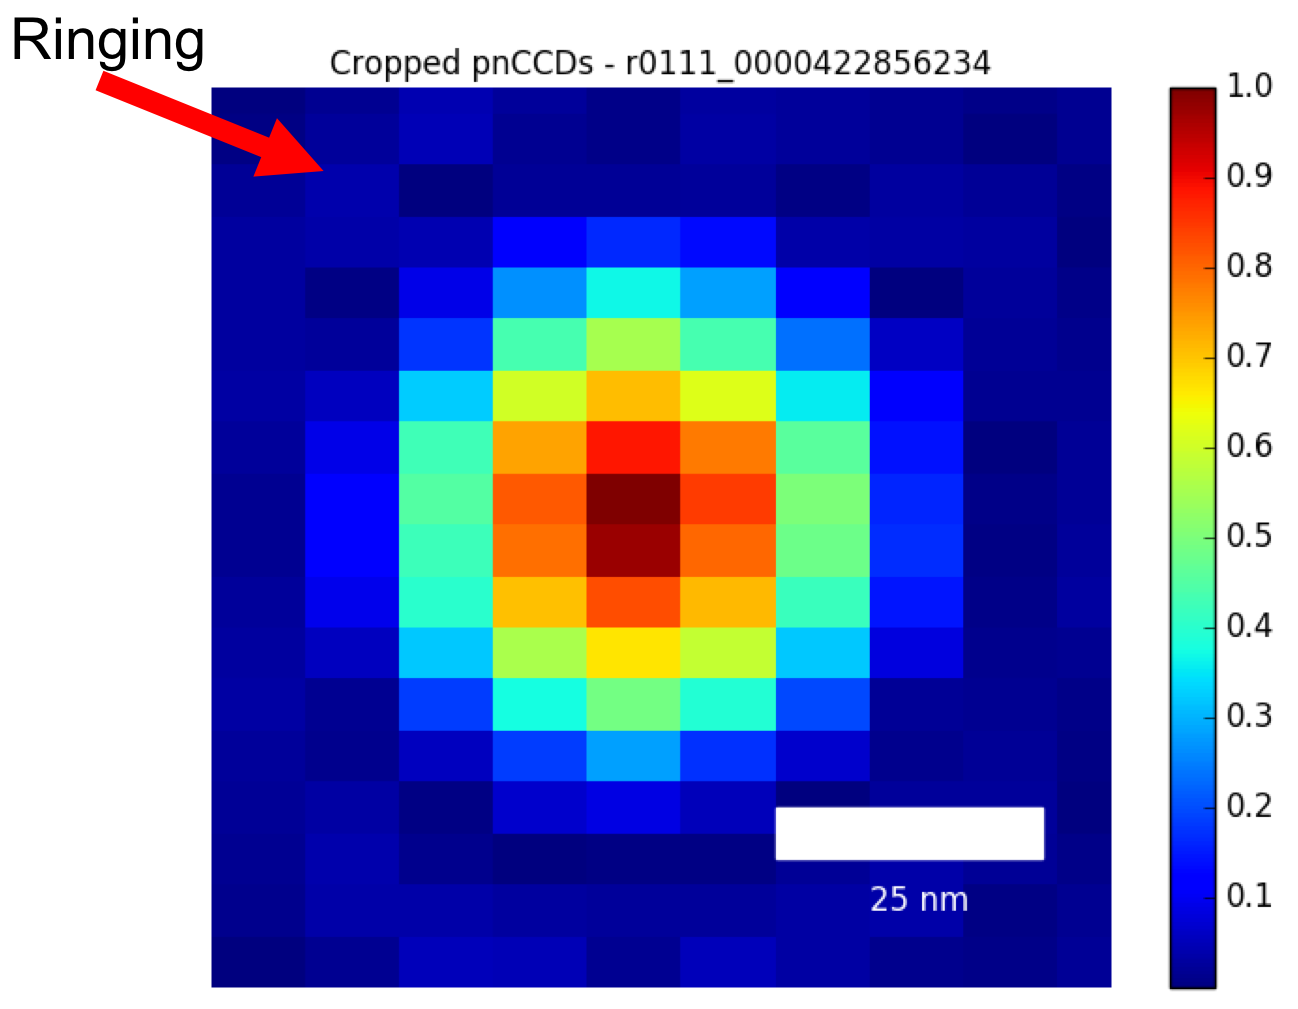
\includegraphics[width=0.53\textwidth]{images/results/Xe_800_fs_ringing.png}
	\caption[Single-shot 2D reconstructions of \SI{\sim 25}{\nano\meter} radius Xe-clusters.]{Single-shot 2D reconstructions of diffraction patterns from single Xe-clusters. The left image shows a \SI{\sim 25}{\nano\meter} radius Xe-cluster at a pump--probe delay $\Delta t=$ \SI{0}{\femto\second}. The cluster has a spherical or arguably icosahedral electron density distribution that is distinct compared to the background. The right image shows a \SI{\sim 25}{\nano\meter} radius Xe-cluster at a time delay $\Delta t=$ \SI{800}{\femto\second} that shows a similar shape. Possibly due to the loss of scatterers (see Figure \ref{fig:number-of-scatterer}) the signal-to-noise ratio decreases and a ringing appears that is likely generated by the support structure in the iterative process.}
	\label{fig:Xe-2D-reconstructions}
\end{figure}
To move beyond modeling diffraction patterns, reconstruction algorithms (see Section \ref{sec:phase-retrieval}) are employed to directly investigate electron density profiles. Figure \ref{fig:Xe-2D-reconstructions} shows 2D reconstructions of single Xe-clusters for the pump--probe delay $\Delta t =$ \SI{0}{\femto\second} (left) and $\Delta t=$ \SI{800}{\femto\second} (right). The clusters appear generally spherical. Both clusters have a radius of $r\approx$ \SI{25}{\nano\meter}. It is noted that the reconstructions therefore constitute some of the smallest objects recovered with diffraction imaging at the time of writing. The minimal resolvable feature size in these images is \SI{\sim 14 x \sim 6}{\nano\meter} along the $X \times Y$-axis (see Section \ref{sec:resolution-discussion}) and therefore, the real-space images are the highest-resolution reconstructions achieved at the time of writing. The reconstruction at $\Delta t=$ \SI{800}{\femto\second} shows a subtle ringing around the actual cluster, which is likely an artifact of the spherical support structure. This ringing becomes visible due to a lower signal-to-noise ratio, which could be due to the described loss of electrons in the interaction region and the therefore overall less scattered light. Due to the current instrumentation-based resolution limitations, a nanoplasma expansion, i.e., the earlier discussed \SI{20}{\percent} increase in Xe-cluster radius, are difficult to reveal in a 2D reconstruction. Also, 2D reconstructions of nanoparticles that have a size of few ten nanometers are challenging and the number of successful 2D reconstructions is low. An alternative approach is to perform 1D reconstructions of the centro-symmetric diffraction images, which have a better signal-to-noise ratio.\\[1\baselineskip]
% 1D RECONSTRUCTIONS
\begin{figure}
	\centering
		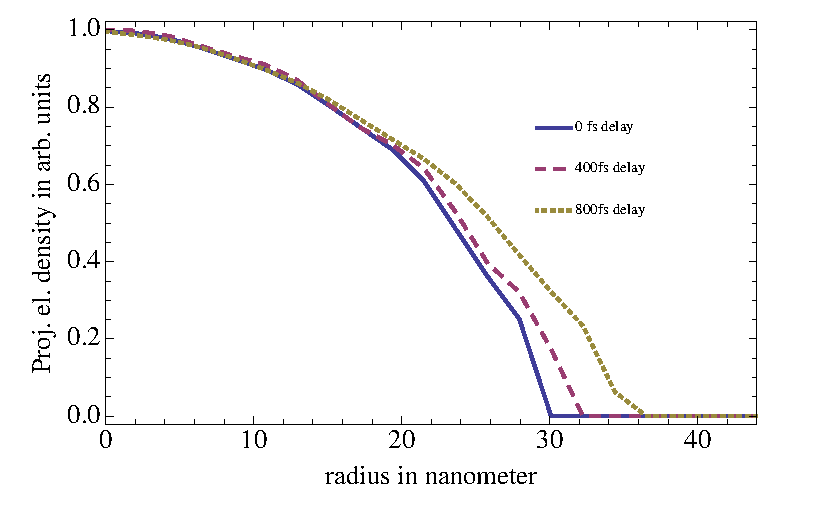
\includegraphics[width=0.80\textwidth]{images/results/Xe-reconstructions.eps}
	\caption[Single-shot 1D reconstruction of \SI{\sim 30}{\nano\meter} radius Xe-cluster]{Single-shot 1D reconstruction of Xe-clusters at various time delays $\Delta t$. The figure shows the projected and normalized el. mass as a function of the radius, i.e., the electron density. These real-space images of a nanoplasma transition show that, at first, outer atomic layers are shed off, here imaged at $\Delta t=400$ fs. And over time, more inner atomic layers follow, here imaged at $\Delta t= 800$ fs.}
	\label{fig:Xe-reconstructions}
\end{figure}
%TO MOVE ON 1D reconstructions of single xenon cluster were obtained as described in Section \ref{sec:1d-proj-and-phase-reconstruction}. Figure \ref{fig:Xe-reconstructions} shows 1D reconstructions of the projected electron density from single xenon cluster at time delays $\Delta t=\{0, 400, 800\}$ fs between the X-ray pump and X-ray probe beam. The density curves are normalized to clearly indicate an expansion of the outer atomic layers of the cluster. In this selection of hits, the cluster radii expand by $\sim 20\%$ over a time delay of $\Delta t=800 fs$, which is a substantial structural change. To make these events COMPARABLE INCLUDE DIFFRACTION PATTERNS. ELECTRON TEMPERATURE\\
1D real-space electron density reconstructions of single Xe-clusters are shown in Figure \ref{fig:Xe-reconstructions} (see Section \ref{sec:1d-proj-and-phase-reconstruction}). The 1D reconstructions show normalized and projected electron density from single xenon cluster at time delays $\Delta t=$ \SIlist{0;400;800}{\femto\second}. At $\Delta t = 0$ fs, the electron density follows the density projection of a sphere (compare Figure \ref{fig:cluster-generation}). With a delay of $\Delta t = 400$ fs, an expansion of the outer atomic layers of the cluster is observed. At $\Delta t = 800$ fs, outer layers continue to expand and inner atomic layers start to follow. Over the time delay sequence $\Delta t=$ \SIrange{0}{800}{\femto\second}, the cluster radius expands \SI{\sim 20}{\percent}, or from $r\approx$ \SIrange{30}{36}{\nano\meter}. This sequence of events gives insight into the shape of the Xe-cluster as it undergoes the nanoplasma expansion and directly shows surface softening of the cluster. This expansion is similar to the modeled surface softening of Reference \cite{Gorkhover-2016-NatPho} and theoretically predictions, e.g., Reference \citep{Hau-Riege-2004-PRE}.\\[1\baselineskip]
%The imaged clusters have comparable initial sizes at the point of injection as they are selected from the lower end of the cluster-size distribution.
% AMPLITUDE AND PHASE DISCUSSION
\begin{figure}
	\centering
		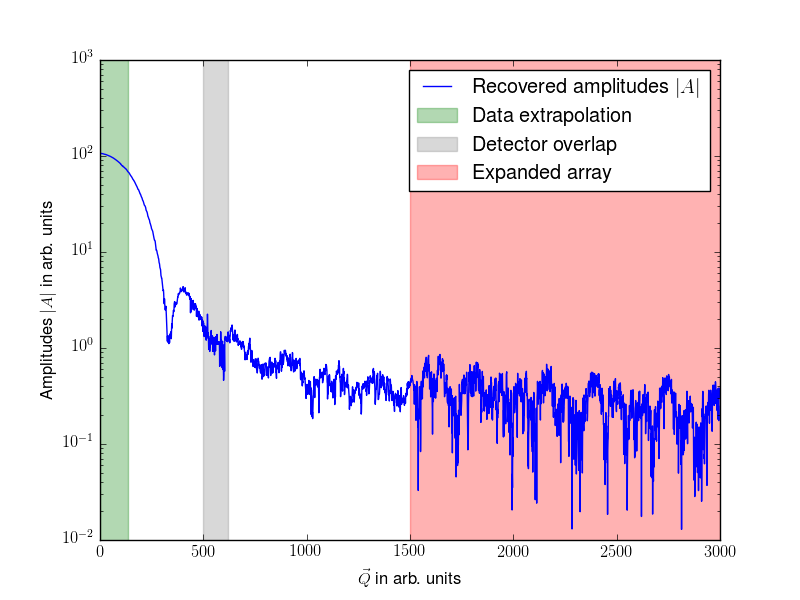
\includegraphics[width=0.49\textwidth]{images/results/amplitude-discussion.png}
		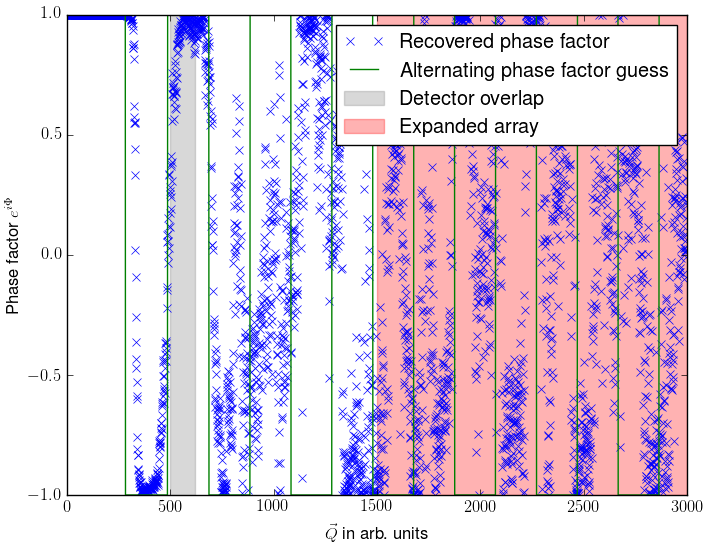
\includegraphics[width=0.49\textwidth]{images/results/phase-discussion.png}
	\caption[Recovered Amplitudes $\lvert A\rvert$ and phase factor of 1D reconstruction]{The left panel shows the recovered amplitudes $\lvert A\rvert$ and the right panel shows the phase factor of the 1D phase retrieval. The green and red background indicates the space where initial data points were extrapolated. The gray area discloses the detector overlap. See Section \ref{sec:1d-proj-and-phase-reconstruction} for more details.}
	\label{fig:amplitude-phase}
\end{figure}
For the sake of completeness of these 1D reconstructions, the recovered modulo of the amplitude, $\lvert A\rvert$, and the recovered phase factor are shown in Figure \ref{fig:amplitude-phase} for the data at $\Delta t =$ \SI{800}{\femto\second}. The amplitudes $\lvert A\rvert$ have been replaced in the space with white background. The data with the green background are interpolated using the anticipated scattering of a sphere. The grayed area indicates the pnCCD detector overlap and the red background data are extrapolated from the scattering of a sphere. The red area therefore artificially increases the resolution. The data points of the k-times iterated Fourier-space function $G'_{k}(\vec{Q})$ in the white area were replaced with the original data set while $G_{k}(\vec{Q})$ was allowed to evolve freely in the remaining area. The phase factor retrieval starts with an initial guess of alternating signs per diffraction ring of the sphere and then evolves freely. One can see how the recovered phase factor is alternating as one would expect from the scattering of a sphere \cite{Guinier-1955-JWS}.
%
%
%
\subsection{X-ray induced damage in pristine He-cluster}\label{sec:He-data-real}
%
\begin{figure}
	\centering
		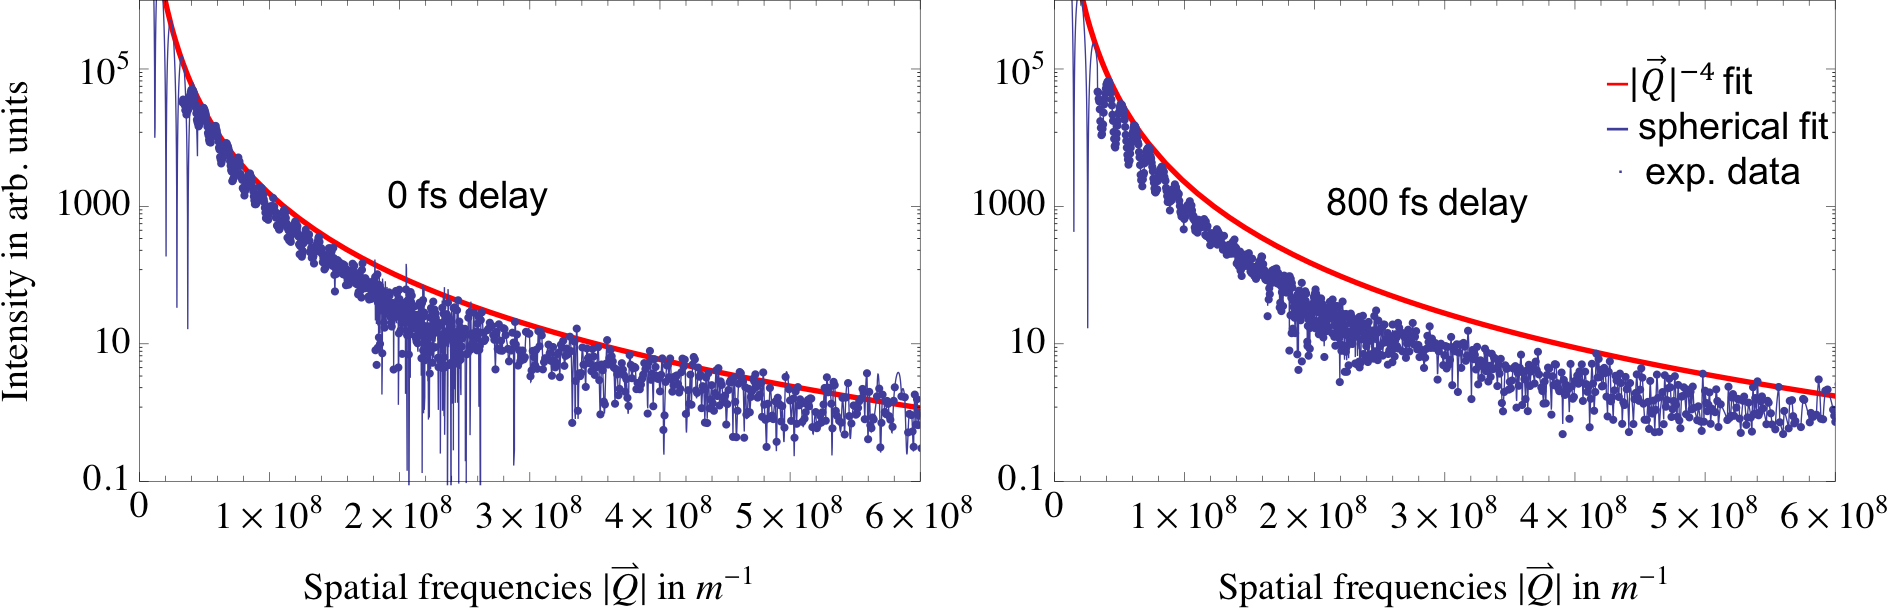
\includegraphics[width=1.00\textwidth]{images/results/He-diffraction-patterns2.png}
	\caption[Single-shot diffraction images of He-droplets at different time delays]{Single-shot diffraction images of pristine He-droplets at various $\Delta t$ spherically projected into 1D.}
	\label{fig:He-diffraction-patterns}
\end{figure}
%
He-droplets have been subject to previous static investigations at the AMO instrument of the LCLS. After injection via a cryogenic cooled source (see Section \ref{sec:sample-delivery}) the superfluid He-cluster \cite{Gomez-2011-JCP} form interesting quantum states \cite{Toennies-2004-ACIE,Gomez-2012-PRL}. Particularly the analysis of their shape shows that droplets form as spheres but also as ellipses \cite{Bernado-2017-PRB}. The ellipticity of a He-droplet relates to its rotational speed. It has been found that rotational speeds of superfluid He-droplets can go beyond the classical stability limits. They are stabilized by quantum vortices, which form inside the He-droplet \cite{Gomez-2014-Science}. For this thesis, only He-droplets that have a spherical form have been selected to avoid quantum vortices. It also enables us to use the symmetry in the diffraction patterns as above and perform a 1D analysis of the diffraction patterns.
%beyond the classical stability limits can be found. 
%As a result, quantum vortices form inside the He-droplet \cite{Gomez-2014-Science}. To not get into too much detail here, for this thesis experiment He-droplets have been selected that have a spherical form. The form of a He-droplet can be easily deduced from the diffraction images thus avoiding the quantum vortices and enabling the analysis of diffraction patterns in 1D as discussed above.
%
Single-shot diffraction images of He-droplets are shown in Figure \ref{fig:He-diffraction-patterns}. The He-droplets have a radii of $r\approx$ \SIlist{379;302}{\nano\meter}, at time delays $\Delta t=$ \SIlist{0;800}{\femto\second}, respectively. For clarity, only the experimental data (blue points), spherical extrapolation at low $\lvert\vec{Q}\rvert$-values (blue line) and the envelope of the spherical extrapolation function (red line) are shown. For $\Delta t =$ \SI{0}{\femto\second}, the local maxima of the experimental data agree well with the envelope function up to very high $\lvert\vec{Q}\rvert$ at the edge of the detector. This indicates an intact He-droplet, as shown in more detail in Section \ref{sec:xenon-data} for Xe-clusters. For a time delay of $\Delta t=$ \SI{800}{\femto\second}, the diffraction pattern of the droplet shows that the local maxima between $\lvert\vec{Q}\rvert \approx$ \SIrange[scientific-notation=fixed, fixed-exponent=8]{1e8}{4e8}{\per\meter} are well below the envelope, this indicates X-ray induced sample damage and is similar to the surface softening discussed above. However, the surface softening of this droplet is less severe as in the Xe-clusters (compare Section \ref{sec:comparison-of-He-and-HeXe-clusters}).
%As shown above, if the scattered intensity distribution of a sphere at large spatial frequencies, $\lvert\vec{Q}\rvert \approx$, is reduced, this indicates X-ray induced sample damage. This is similar to the surface softening discussed above, however, the surface expansion speed is less quickly than in the Xe-clusters. This has been quantify in more detail in Section \ref{sec:comparison-of-He-and-HeXe-clusters}. 
A phenomenological approach to explain the difference in sample damage is that the absorption cross-section of the helium atoms is much smaller than the one of xenon (see Section \ref{tab:helium-xenon-ionization}).
%
%
%
%
\subsection{Condensation of xenon in helium cluster: Plum-pudding type cluster}\label{sec:helium-data}
%%%%%%%%%%%%%%%%%%%%
% - Presentation of He data
%%%%%%%%%%%%%%%%%%%%%%%%%%
%
When this thesis experiment was designed there was the hypothesis that Xe-atoms inside the He-droplets agglomerate to one compact structure with solid density. While it was known that for weak doping levels, the Xe-atoms condense to clusters with multiple centers \cite{Loginov-2011-PRL,Gomez-2014-Science} it was hypothesized that higher Xe-doping levels favor the formation of a single Xe-cluster inside the He-droplet. This is called a xenon core--helium shell system. Figure \ref{fig:HeXe-cluster-diff-patttern} shows a typical diffraction pattern of a HeXe-cluster at \SI{0.5}{\percent} Xe-doping level. The diffraction image immediately indicates a more complex structure of the Xe-particles within a spherical He-droplet than possible with a single Xe-core.
%
\begin{figure}
 	\centering
 		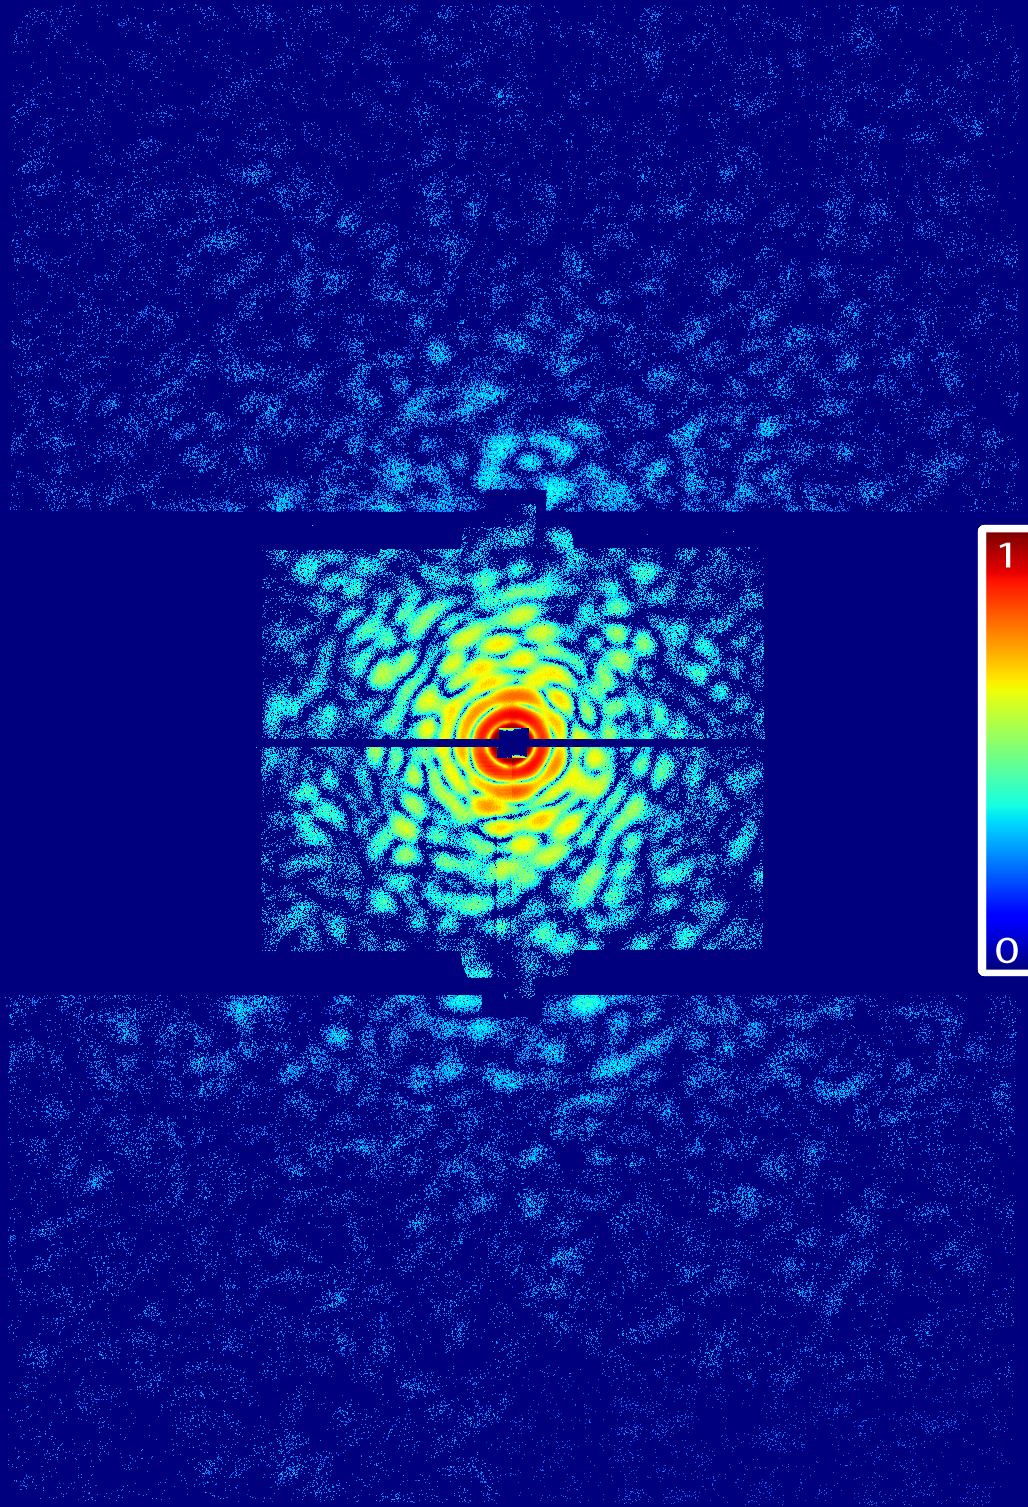
\includegraphics[width=0.93\textwidth]{images/results/HeXediffPattern-113-05-doping-diffpattern2.png}
 	\caption[Diffraction image of HeXe-cluster at \SI{0.5}{\percent} Xe-doping.]{Diffraction image of a HeXe-cluster that has a radius of $r\approx$ \SI{210}{\nano\meter} and a Xe-doping level of \SI{\sim 0.5}{\percent}. The image indicates a complex structure of Xe-particles within a spherical He-droplet. The corresponding real-space reconstruction is shown in Figure \ref{fig:HeXe-cluster-60}.}
 	\label{fig:HeXe-cluster-diff-patttern}
\end{figure}
%
%It is not well known how heterogeneous helium-xenon clusters form a core-shell system. As described in Section \ref{sec:heterogeneous-cluster}, the superfluid helium cluster picks up xenon atoms as it traverses the doping unit. The xenon atoms move unhindered in the superfluid helium and eventually the xenon atoms condense to energetically favorable cluster structures. Reference \citep{Gomez-2014-Science} reports that at a doping level of \SI{0.02}{\percent}, i.e., when there are 5000 more helium atoms than xenon atoms, multiple smaller clusters form and locate at vortexes within a rotating helium droplet.However, it is unknown how xenon atoms arrange in non-rotating droplets and also at higher doping levels.
A first step is therefore to investigate the morphology of Xe-clusters in He-droplets in more detail and create a model for the complex structure of HeXe-cluster. For this, we can state two competing hypotheses: one, xenon atoms condense to one large cluster within a helium droplet; and two, multiple smaller Xe-clusters form within a droplet. Let us call hypothesis two a \textit{plum-pudding core--shell system}\footnote{The name plum-pudding model comes from J.J. Thomson's model of the atom in 1904 and has here been reused to describe the arrangement of Xe-particles in He-droplets.} that we can further divide into a case of few scatterers and many scatterers.\\[1\baselineskip]
%
\begin{figure}
 	\centering
 		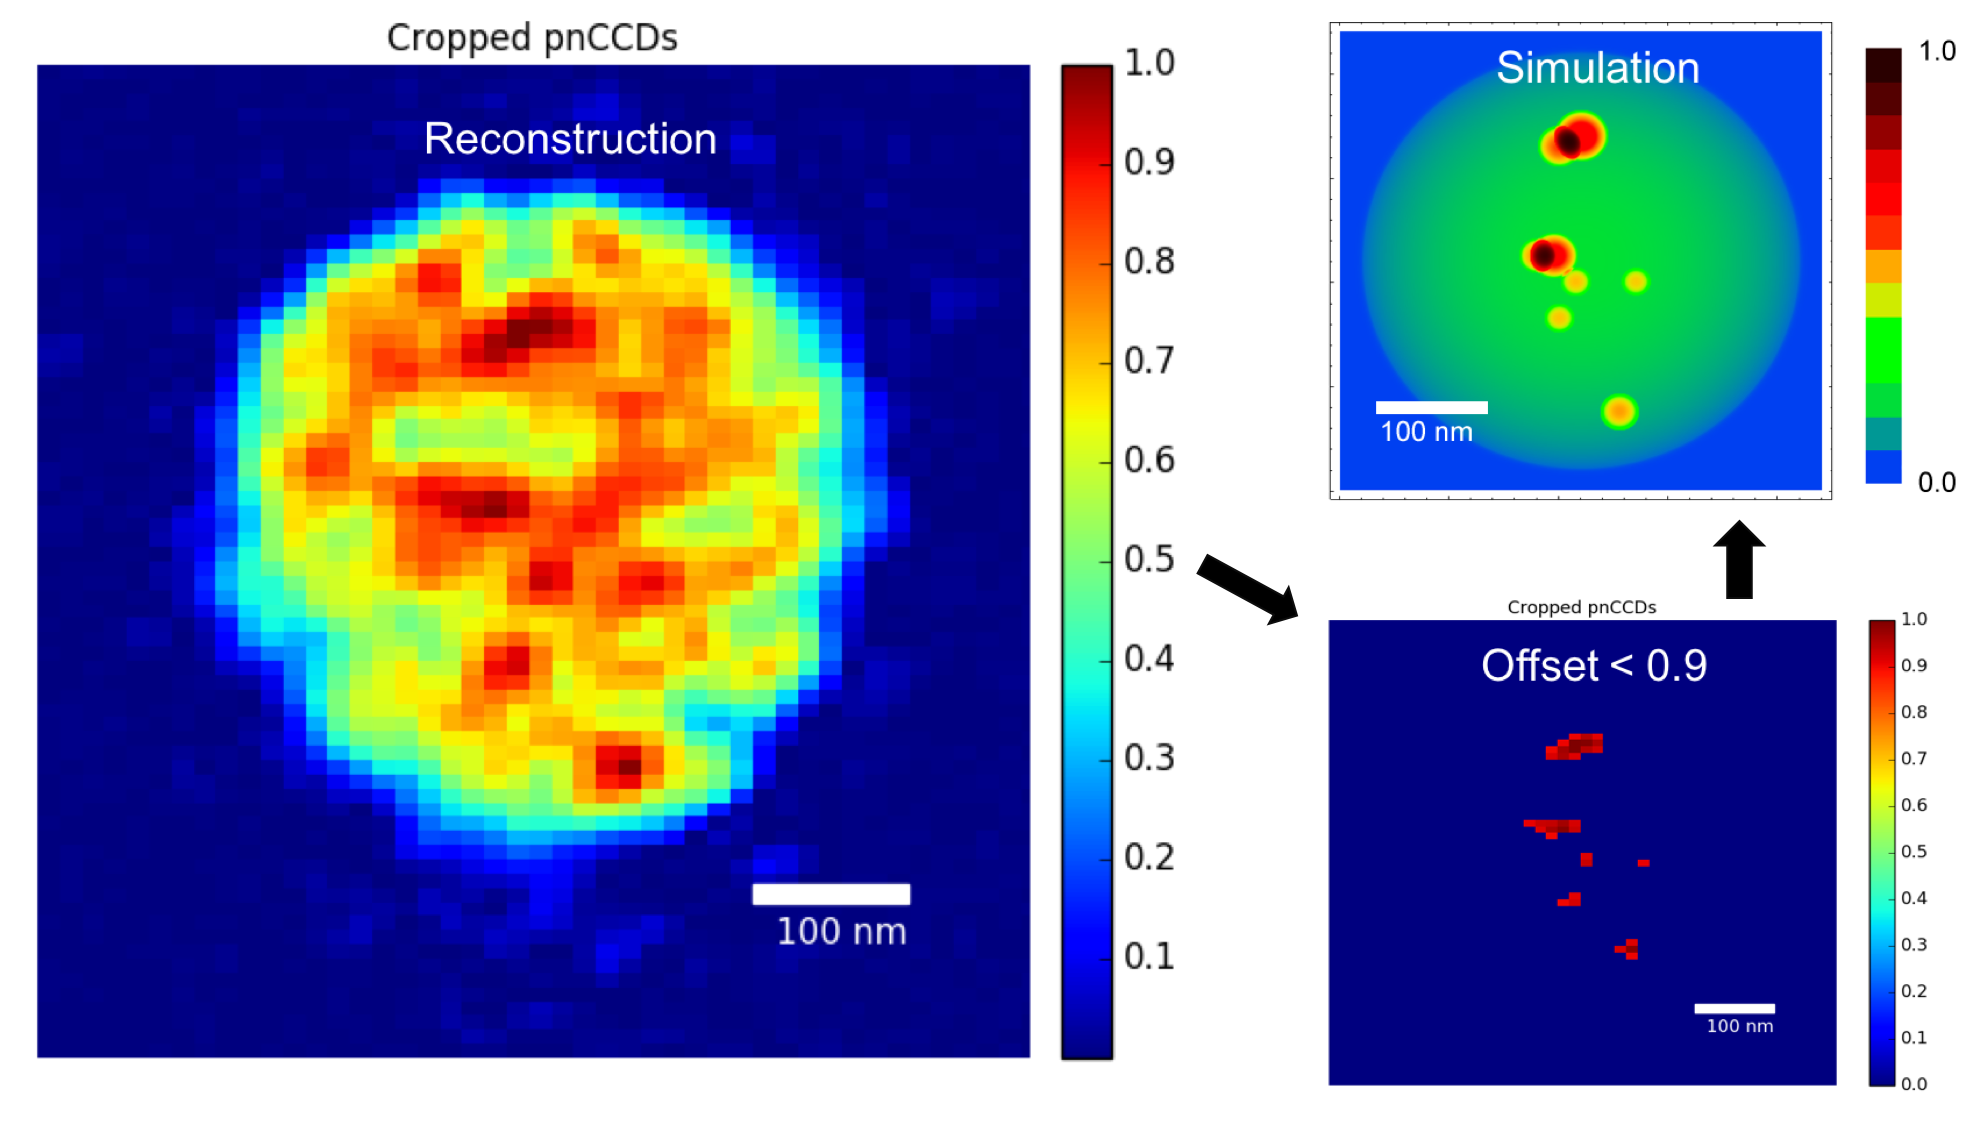
\includegraphics[width=0.80\textwidth]{images/results/reconstructions-to-simulations_new.png}
 	\caption[From a HeXe-cluster reconstruction to a simulated electron density.]{From a HeXe-cluster reconstruction to a simulated electron density. The real-space reconstruction of a HeXe-cluster has a radius of $r\approx$ \SI{210}{\nano\meter} and a Xe-doping level of \SI{\sim 0.5}{\percent} (left). The normalized intensity map is offset (bottom right image) and mimicked by 2D electron density simulations (top right image). The electron density indicates a Xe-cluster arrangement inside the He-droplet of the plum-pudding few scatterers case as discussed in Figure \ref{fig:HeXe-plum-pudding}.}
 	\label{fig:HeXe-cluster-60}
\end{figure}
%
To investigate this hypothesis, real-space reconstructions from single-shot diffraction images of HeXe-clusters are analyzed first. The left panel of Figure \ref{fig:HeXe-cluster-60} shows a reconstruction of a HeXe-cluster that has a radius of $r\approx$ \SI{210}{\nano\meter} and a Xe-doping level of \SI{\sim 0.5}{\percent}. The reconstruction indicates a plum-pudding arrangement, where a few Xe-clusters (intense, dark red spots) are randomly distributed within the He-droplet (less intense, green to orange area). In the bottom right panel of Figure \ref{fig:HeXe-cluster-60}, the normalized intensity map from the reconstruction is offset to guide the eye to dense centers. These dense centers can be used to model an electron density in the 2D-simulations that are discussed in Section \ref{sec:2d-simulations}. The top right panel of Figure \ref{fig:HeXe-cluster-60} shows the modeled electron densities. These simulated electron densities can be Fourier transformed into reciprocal space and ultimately be compared to the measured data.\\[1\baselineskip]
%
\begin{figure}
 	\centering
 		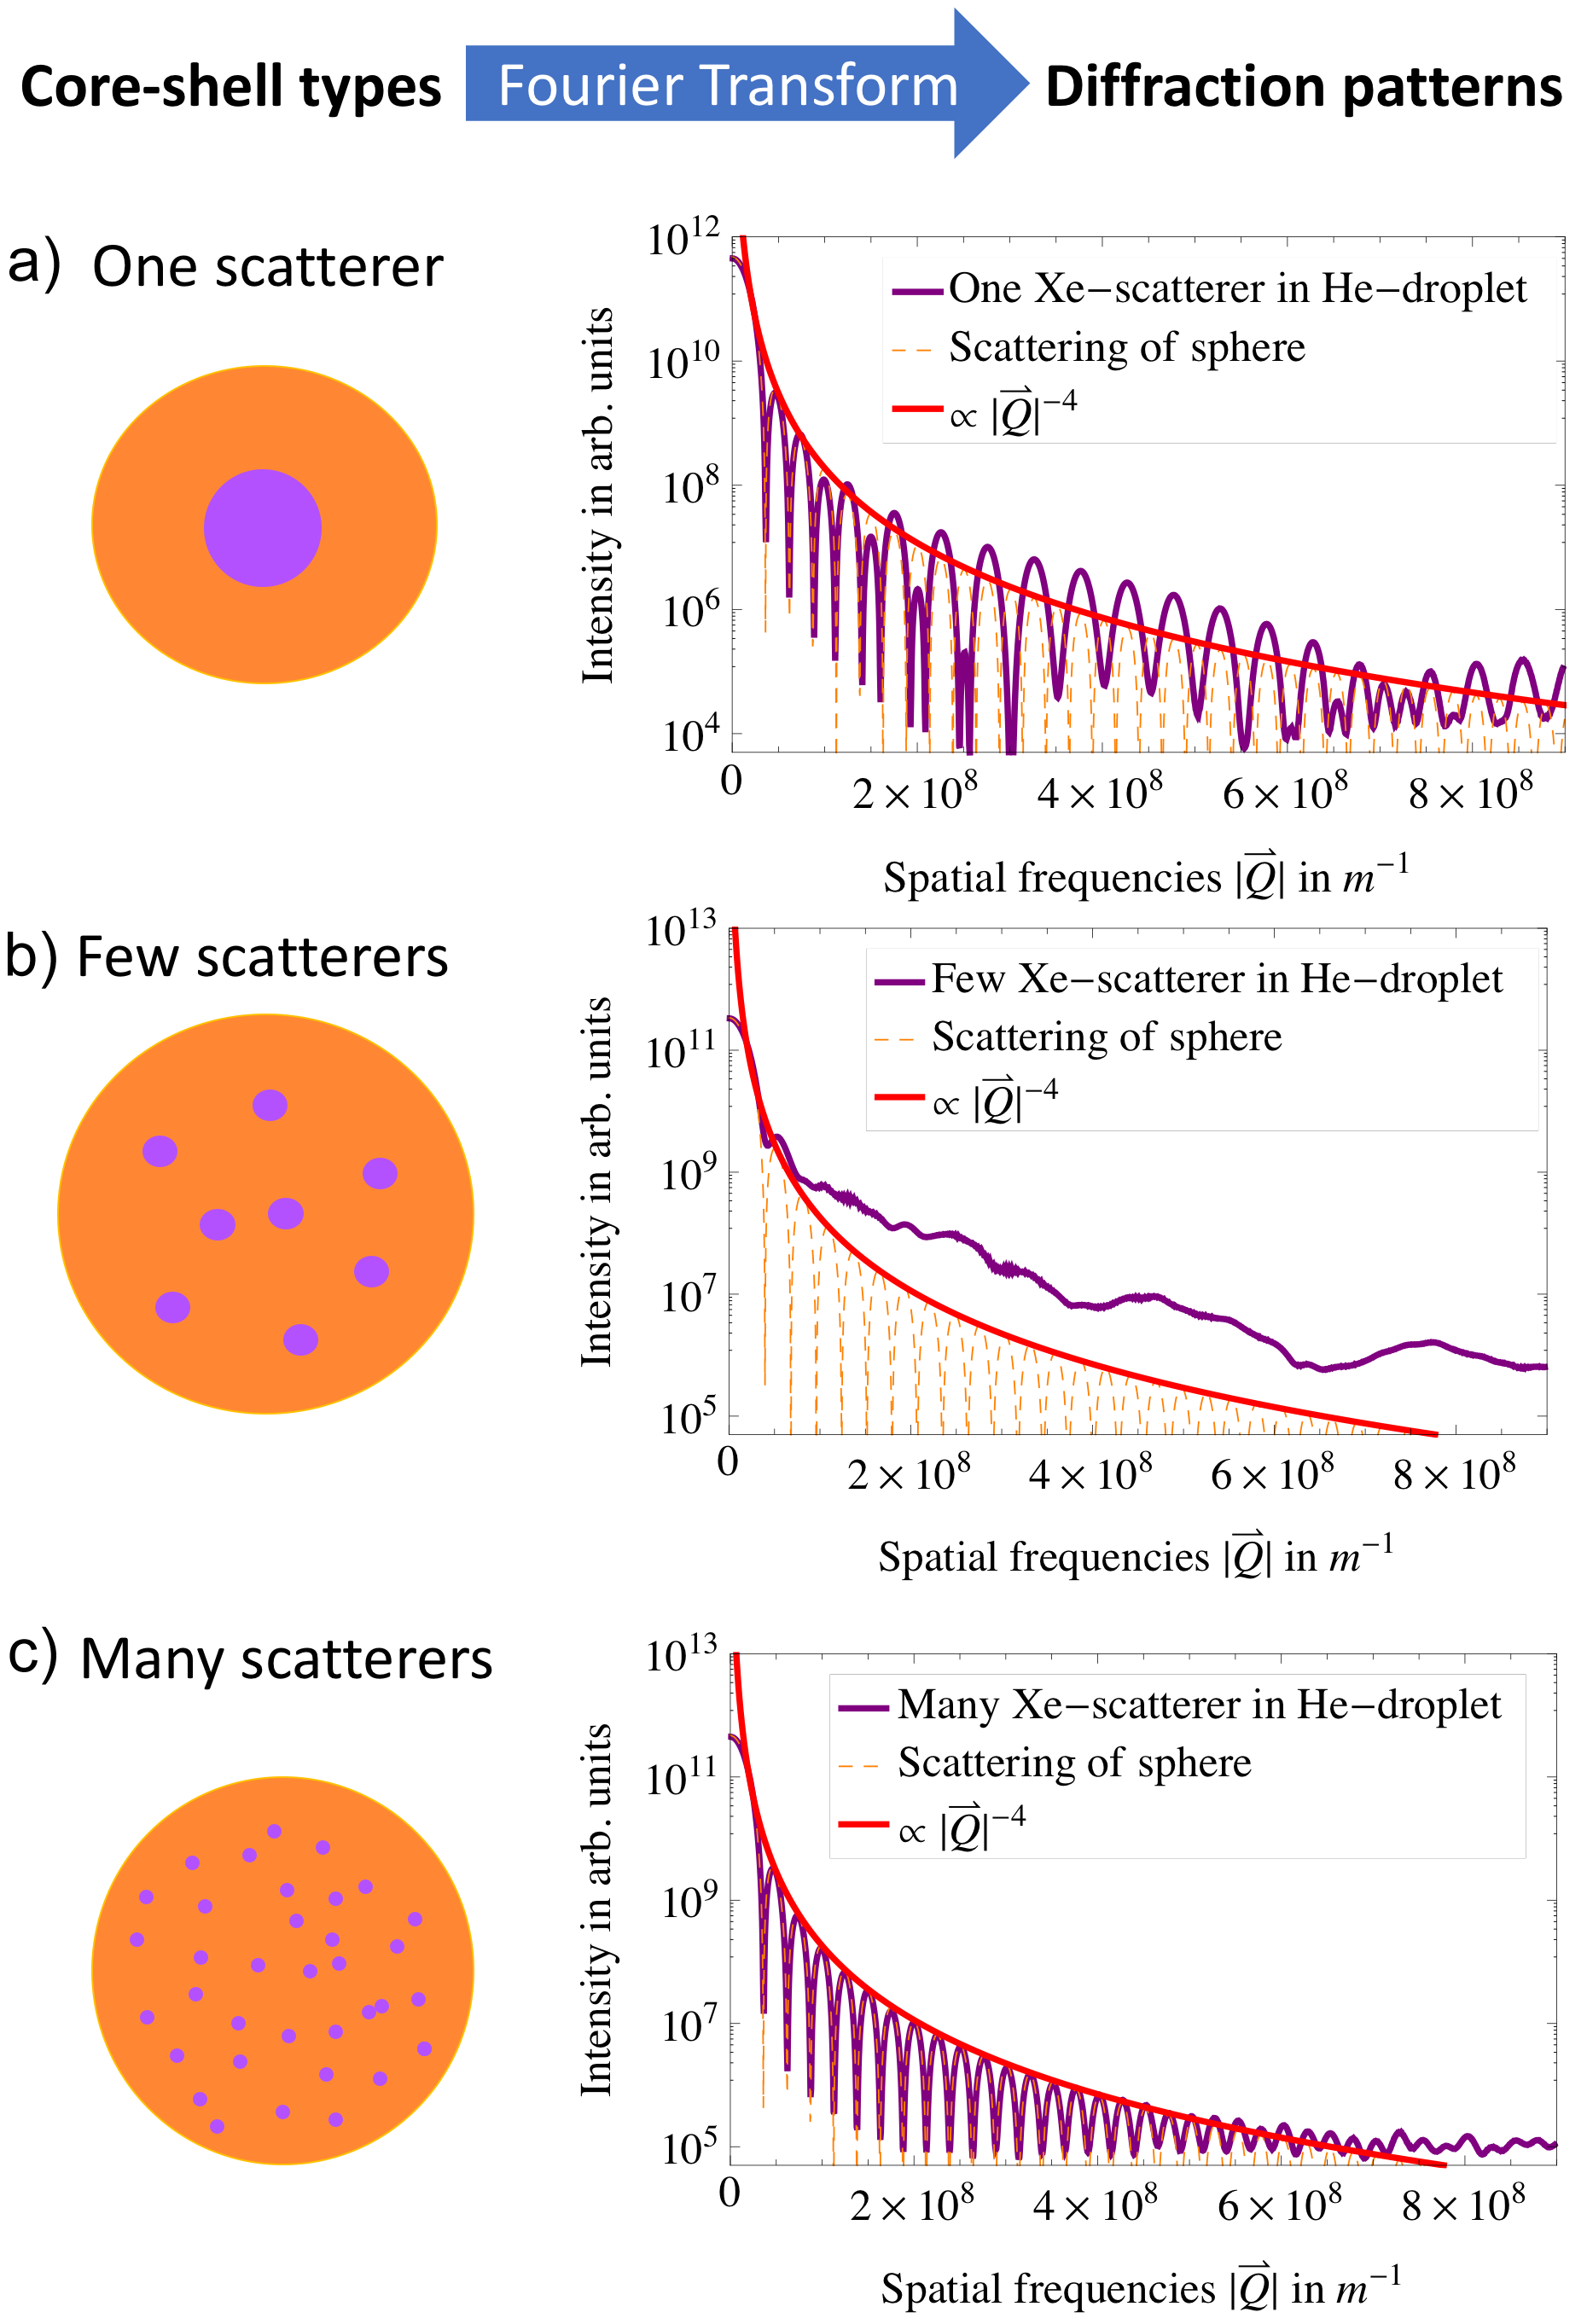
\includegraphics[width=0.82\textwidth]{images/results/plum-pudding_numbered.png}
 	\caption[Hypothetical arrangements of Xe-clusters within He-droplets.]{Hypothetical arrangements of Xe-clusters in superfluid He-droplets (left) and corresponding 1D diffraction patterns (right). The He-droplet has a radius of \SI{\sim 125}{\nano\meter} and the Xe-doping level is \SI{\sim 20}{\percent}. The case of one xenon scattering center $N_{\text{sc}}=1$ (top), few scatterers $N_{\text{sc}}=8$ (middle), and many scatterers $N_{\text{sc}}=100$ (bottom) are shown. The scattering pattern is dominated by the signal from the He-droplet at low spatial frequencies, but at large $\lvert\vec{Q}\rvert$-values the signal is dominated by the Xe-clusters. This is mostly due to the size of the Xe-clusters; smaller scattering centers are resolved at larger scattering angles.}
 	\label{fig:HeXe-plum-pudding}
\end{figure}
To verify the success of the HeXe-reconstruction and to further test the above stated hypothesis, several core-shell simulations are discussed next. Figure \ref{fig:HeXe-plum-pudding} shows the discussed core--shell scenarios along with their Fourier-space representations in 1D. The simulated He-droplet has a radius of $r_{\text{He}}\approx$ \SI{125}{\nano\meter} and a constant Xe-doping level of \SI{\sim 20}{\percent}. As comparison, the yellow, dashed line in the figure describes the scattered intensity distribution of this sphere and the red line is its envelope function. The figure depicts an artistic representation of the actual simulated electron densities from the core--shell systems on the left side. On the right side, the Fourier transformed data reveal that the agglomeration of the Xe-particles within the He-droplet dominates the scattering pattern (purple curve). This is due to the Xe-cluster density being \num{\sim 25.8} times larger than the density of liquid He-droplets and the resulting scattering factors that were discussed in Table \ref{tab:helium-xenon-el-scattering-crossection}. In the one-scatterer case with a single centered scattering center (see Figure \ref{fig:HeXe-plum-pudding}a), $N_{\text{sc}}$, the purple curve consists of a large modulation in the diffraction image, which comes from the Xe-core and a small, more intense modulation that comes from the He-shell. The small modulation is similar to the yellow, dashed line and at low spatial-frequencies, where the He-droplet dominates the signal on the diffraction image. At large spatial-frequencies, the modulation from the Xe-cluster is more prominent. Ultimately, this is related to the size and density of each cluster, which is discussed in more detail below. In the few scatterers case with $N_{\text{sc}}=8$ scattering centers (see Figure \ref{fig:HeXe-plum-pudding}b), the diffraction pattern (purple line) at low spatial-frequencies $\lvert\vec{Q}\rvert$ is still dominated by the He-shell and at high spatial-frequencies $\lvert\vec{Q}\rvert$ by the Xe-cores. However, the diffraction image appears to contain a more complex structure at large $\lvert\vec{Q}\rvert$-values due to the delocalized scatterers. Also, the average scattering intensity is well above the envelope of the scattering of a sphere (red line). The exact location of the few scattering centers has a small effect to the 1D projection of the 2D diffraction image, as long as the scattering centers are distributed throughout the He-droplet. In the many scatterers case with $N_{\text{sc}}=100$ (see Figure \ref{fig:HeXe-plum-pudding}c), the scattering centers are randomly distributed within the He-droplet. The Xe-clusters are significantly reduced in size to match the constant xenon doping level of \SI{\sim 20}{\percent}. For the shape of the HeXe-cluster, the small clusters appear similar to a constant electron density increase, which is why the scattering is similar to the scattering of a sphere (yellow, dashed line) at low-to-mid $\lvert\vec{Q}\rvert$-values. Only at large spatial frequencies, $\lvert\vec{Q}\rvert$, which carry signal of high-resolution, the small Xe-particle structures are revealed and start to dominate the pattern.\\[1\baselineskip]
%
The cases of the one scatterer and the many scatterers case show a rather simple structure in reciprocal space and are thus not able to reproduce a scattering image as the one shown in Figure \ref{fig:HeXe-cluster-diff-patttern}. Only the few scatterers case results in a complex structure in reciprocal space. HeXe reconstructions and electron density simulations indicate that HeXe-clusters agglomerate to a plum-pudding core--shell system with a few scattering centers.\\[1\baselineskip]
%
%These cases show rather simple structured diffraction patterns for the one scatterer and many scatterers case and only the few scatterers case results in a complex diffraction image such as the measured one shown in Figure \ref{fig:HeXe-cluster-diff-patttern}. This is another indication that HeXe-cluster agglomerate as few clusters in the pump-pudding core--shell type.\\[1\baselineskip]
%
%Before we move on to match the simulations to the data (see Section \ref{sec:helium-xenon-data}),
As we have seen above, the Xe-clusters dominate the diffraction pattern at least at large angles. Particularly the size of the Xe-clusters plays a major role at which spatial frequencies the Xe-clusters start to dominantly contribute. Let us quantify this finding with an estimation.
%Let us now address the question of how the size of a Xe-cluster changes its contribution to the intensity distribution in reciprocal space at a certain spatial frequency. In other words, can we estimate at which spatial frequency in the diffraction pattern one would expect a significant contribution of a cluster with a given size. 
For this, we can make use of Abbe's criterion (see Equation \eqref{eq:abbe-criterion}) and the wave-vector definition (see Equation \eqref{eq:Q-scattering-angle}). In vacuum, we can note the minimal resolvable feature size $d$ as
\begin{equation}
d = \frac{2\pi}{\lvert\vec{Q_{r}}\rvert},
\label{eq:diameter-estimate}
\end{equation}
with $\lvert\vec{Q_{r}}\rvert$ being the spatial frequency relating to $d$. The feature size corresponds to the radius as $d\approx 2 r$. This relation connects the radius of Xe-clusters to a certain point $\lvert\vec{Q_{r}}\rvert$ in reciprocal space, where the Xe-clusters start to dominantly contribute to the diffraction image. The estimation via this relation works well for the one-scatterer case, where $r_{\text{Xe}}\approx$ \SI{15}{\nano\meter}. However, as the structures become more complex with dense scattering centers throughout the cluster, the contributions to the spatial frequencies become more complex, for example, spatial frequencies originate not only from the size of the dense scattering centers but also their distances to the edges of the droplet and also the distances to other dense scattering centers. Thus, for the few scatterers case, the radii are estimated to be \num{\sim 3} times larger than in the actual simulation. This is similar in the many scatterers case. Here, the spatial frequency domain even more complex due to the many particles, their size variety and distances to surrounding objects such that the estimation overestimates the radii by a factor \num{\sim 10}. If ones desire is to determine the size of an embedded particle, which is a useful feature particularly to test the sample injection process, this can be done easily if just one particle is embedded in the center of the droplet. As multiple particles are embedded in a single He-droplet, this size estimation becomes less accurate.\\[1\baselineskip]
%This superstructure is \num{\sim 3} times larger in the few scatterers case and \num{\sim 10} times larger in the many scatterers case than its individual, simulated Xe-cluster components.
%Multiple smaller structures thus form a \textit{superstructure}\index{superstructure} that appears larger than its individual components when estimated via Equation \eqref{eq:diameter-estimate}. For the plum-pudding cases the Xe-cluster form superstructures with the He-droplet. 
%
%The study of diffraction patterns thus gives insight into the heterogeneous core-shell system. Ultimately, the structure of a heterogeneous HeXe-cluster must be understood to further conclude about effects of radiation damage. To study the diffraction pattern of heterogeneous cluster 2D simulations were developed that simulate the electron density of a cluster and then Fourier transform these into Fourier-space. The 2D diffraction images are then projected onto 1D to be compared efficiently. More details about this method can be found in Section \ref{sec:2d-simulations}.\\
%The 2D electron density simulations show that Xe atoms arrange as few randomly orientated clusters within the He-droplet. The data in Figure \ref{fig:HeXe-cluster-60} shows several cases of Xe arrangement within the He-droplet. First, looking at the extreme cases of no Xe-scatterer (n=0) and many small Xe-scatterer $(n=100)$ show vastly different scattering pattern than measured. Only the case of few Xe-scatterer $(n\approx 10)$ reproduces the in the experiment measured data. This approach also allows a precise determination of the Xe-doping level on a shot-to-shot basis as the size of the Xe-cluster within the He-droplet can be adapted to fit the measurement. The overall amount of Xe in the system can be compared to the amount of He and thus a relative doping level is found. In this example, a doping level of XXX was found. This agrees well with the average doping level calculated in Equation \eqref{eq:average-dopant}.\\
%
%
%
% \subsection{Diffraction images of helium cluster}
%%%%%%%%%%%%%%%%%%%%%%%%%%%%%%%%%%%%%%%
%- Work out radiation damage in 1D diffraction images.\\
%- Introduce envelope to show the radiation damage effect - important to compare to HeXe data.\\
%- Eventually subsection for reconstructions.
%%%%%%%%%%%%%%%%%%%%%%%%%%%%%%%%%%%%%%%
%
%
%
\subsection{Understanding sample damage in the plum-pudding type clusters}\label{sec:helium-xenon-data}
%%%%%%%%%%%%%%%%%%%%%%%%%%%%%%%%%%%%%%
%-Presentation of HeXe data
%%%%%%%%%%%%%%%%%%%%%%%%%%%%%%%%%%%%%%
\begin{figure}
	\centering
		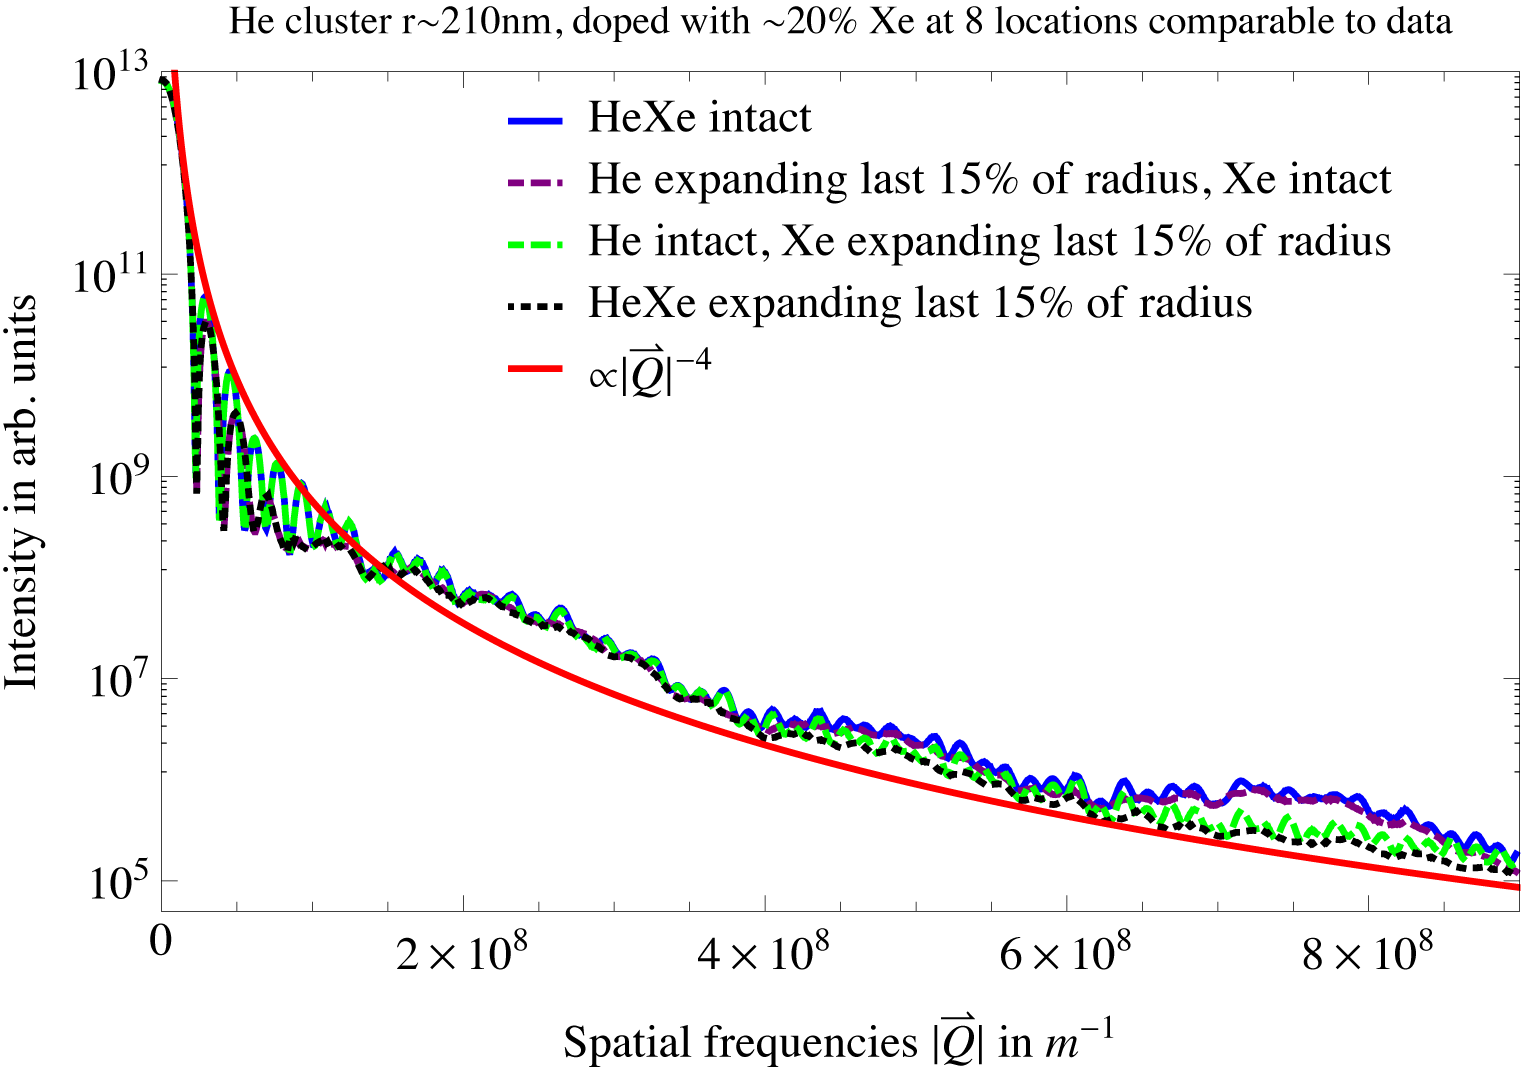
\includegraphics[width=0.95\textwidth]{images/results/simulations-damage-explain3.png}
	\caption[Simulated structural damage scenarios in HeXe-clusters.]{Simulated structural damage scenarios in simulated HeXe-clusters diffraction images. In reciprocal space: The blue curve shows the helium droplet as well as Xe-clusters intact. The purple, dashed curve shows an expanding He-droplet, leaving the Xe-clusters intact. The green, dashed curve leaves the He-droplet intact but shows expanding He-clusters. The black, dashed curve shows both cluster types expanding. The red curve is the envelope of the scattering of a sphere fitted to the zeroth order. The electron density arragement from Figure \ref{fig:HeXe-cluster-60} was used for these simulations and the electron density expansion introduced via Equation \eqref{eq:el-density-expanding-2d}.}
	\label{fig:simulations-damage-explain}
\end{figure}
%
This section investigates the surface softening in plum-pudding type HeXe-clusters. In a first step, 2D simulations are discussed in detail to go over possible sample damage scenarios. In a second step, the 2D simulations are compared to the measured data.
%This section compares the measured diffraction pattern directly to the simulated diffraction pattern, which have been Fourier transformed from the reverse engineered electron densities. Hereby, we will also address the effect of the surface expansion in the heterogeneous system and address this first. 
Figure \ref{fig:simulations-damage-explain} shows a simulated diffraction pattern from the plum-pudding type electron density shown in Figure \ref{fig:HeXe-cluster-60}. The He-droplet has a radius $r_{\text{He}}=$ \SI{210}{\nano\meter} and a strong Xe-doping of \SI{\sim 20}{\percent} to amplify the effects of the sample damage in the diffraction pattern. The figure shows several sample damage scenarios and the effects of this damage to the diffraction pattern. As described in Section \ref{sec:2d-simulations}, the modeled radiation damage is comparable to a surface softening. The blue, solid curve describes the scenario, where all spheres, i.e., clusters, are intact and no X-ray induced dynamics are present. The purple, dashed curve shows the case where the last \SI{15}{\percent} in units of the He-droplet radius, $r_{\text{He}}$, expands but the Xe-cluster are intact. Conversely, the green, dashed curve shows the effect, where the last \SI{15}{\percent} of the radius from Xe-clusters, $r_{\text{Xe}}$, expand but the He-shell stays intact. Lastly, the case, where all spheres are expanding in the last \SI{15}{\percent} of their radii. It can be clearly seen that each scenario leaves a distinct fingerprint. In other words, the expansion of the large He-droplet affects low spatial frequencies and the expansion of small Xe-clusters affects high spatial-frequencies.
%It can be clearly seen that the expansion of each cluster type effects either low spatial-frequencies when the He-droplet is expanding, or high spatial-frequencies when the (much smaller) Xe-cluster are expanding. 
The vast size difference of the Xe-clusters to the He-droplet, which are $r_{\text{Xe}}=$ \SIlist{25;22;20;18;17;14;14;13.5}{\nano\meter} versus $r_{\text{He}}=$\SI{210}{\nano\meter}, allow a separation between the spatial frequency contributions in the diffraction pattern. This separation is related to the estimation made in Section \ref{sec:helium-data}. It is interesting to note how independently the He- and Xe-contributions affect their parts in the diffraction pattern. 
%This separation in the contributions also allows to attribute effects in the diffraction pattern either to the He-droplet or the Xe-clusters. 
%Summarizing the HeXe-cluster simulations. When the He-droplet exhibits a surface softening low spatial frequency contributions are reduced, whereas a surface softening of the Xe-clusters leads to a reduction of high spatial frequency contributions.\\[1\baselineskip]
%Now that we have discussed the effects of X-ray induced dynamics, i.e. radiation damage, in Xe-clusters by analyzing single-shot diffraction pattern and time-of-flight mass spectroscopy and also having understood the structure of heterogeneous HeXe cluster as they arrange in a \textit{plum-pudding} type model, where few Xe-scatterer are present in a large He-droplet, we can discuss the diffraction pattern from the pump--probe data of HeXe-clusters. Let us start off by reusing the 2D simulations, described in Section \ref{sec:2d-simulations}, using damaged spheres to investigate the effects onto the diffraction pattern.\\
\begin{figure}
%width=0.49\textwidth
	\centering
		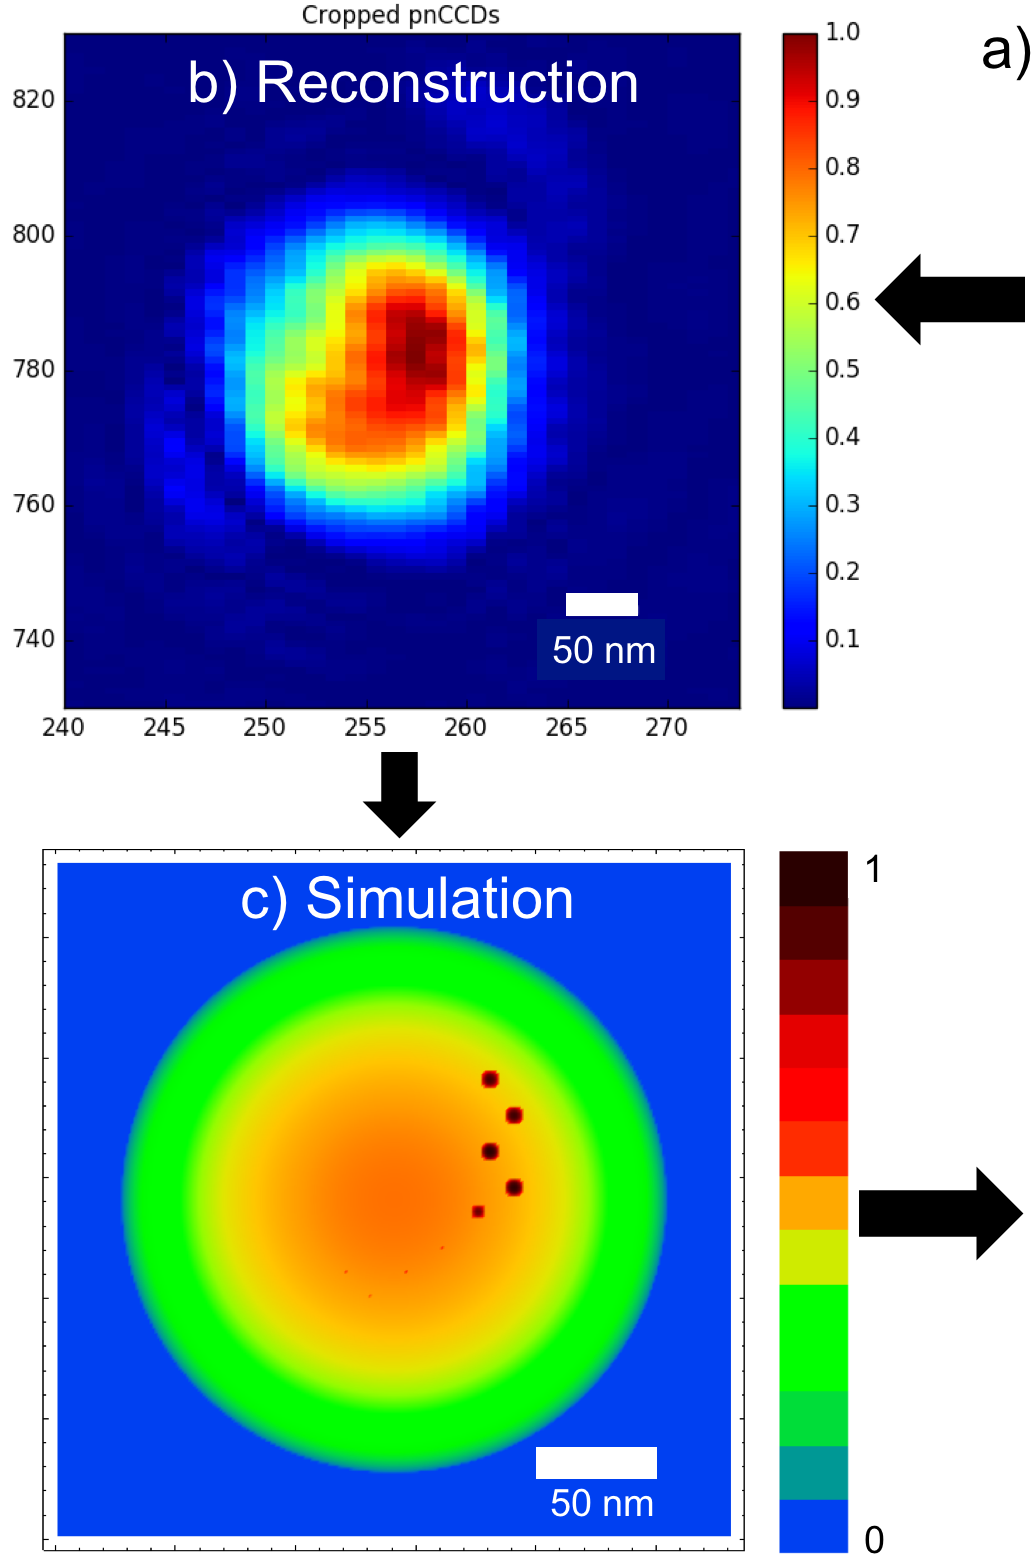
\includegraphics[height=6.0cm]{images/results/HeXe-densities-113-05-doping-and-reconstruction-1.png}
		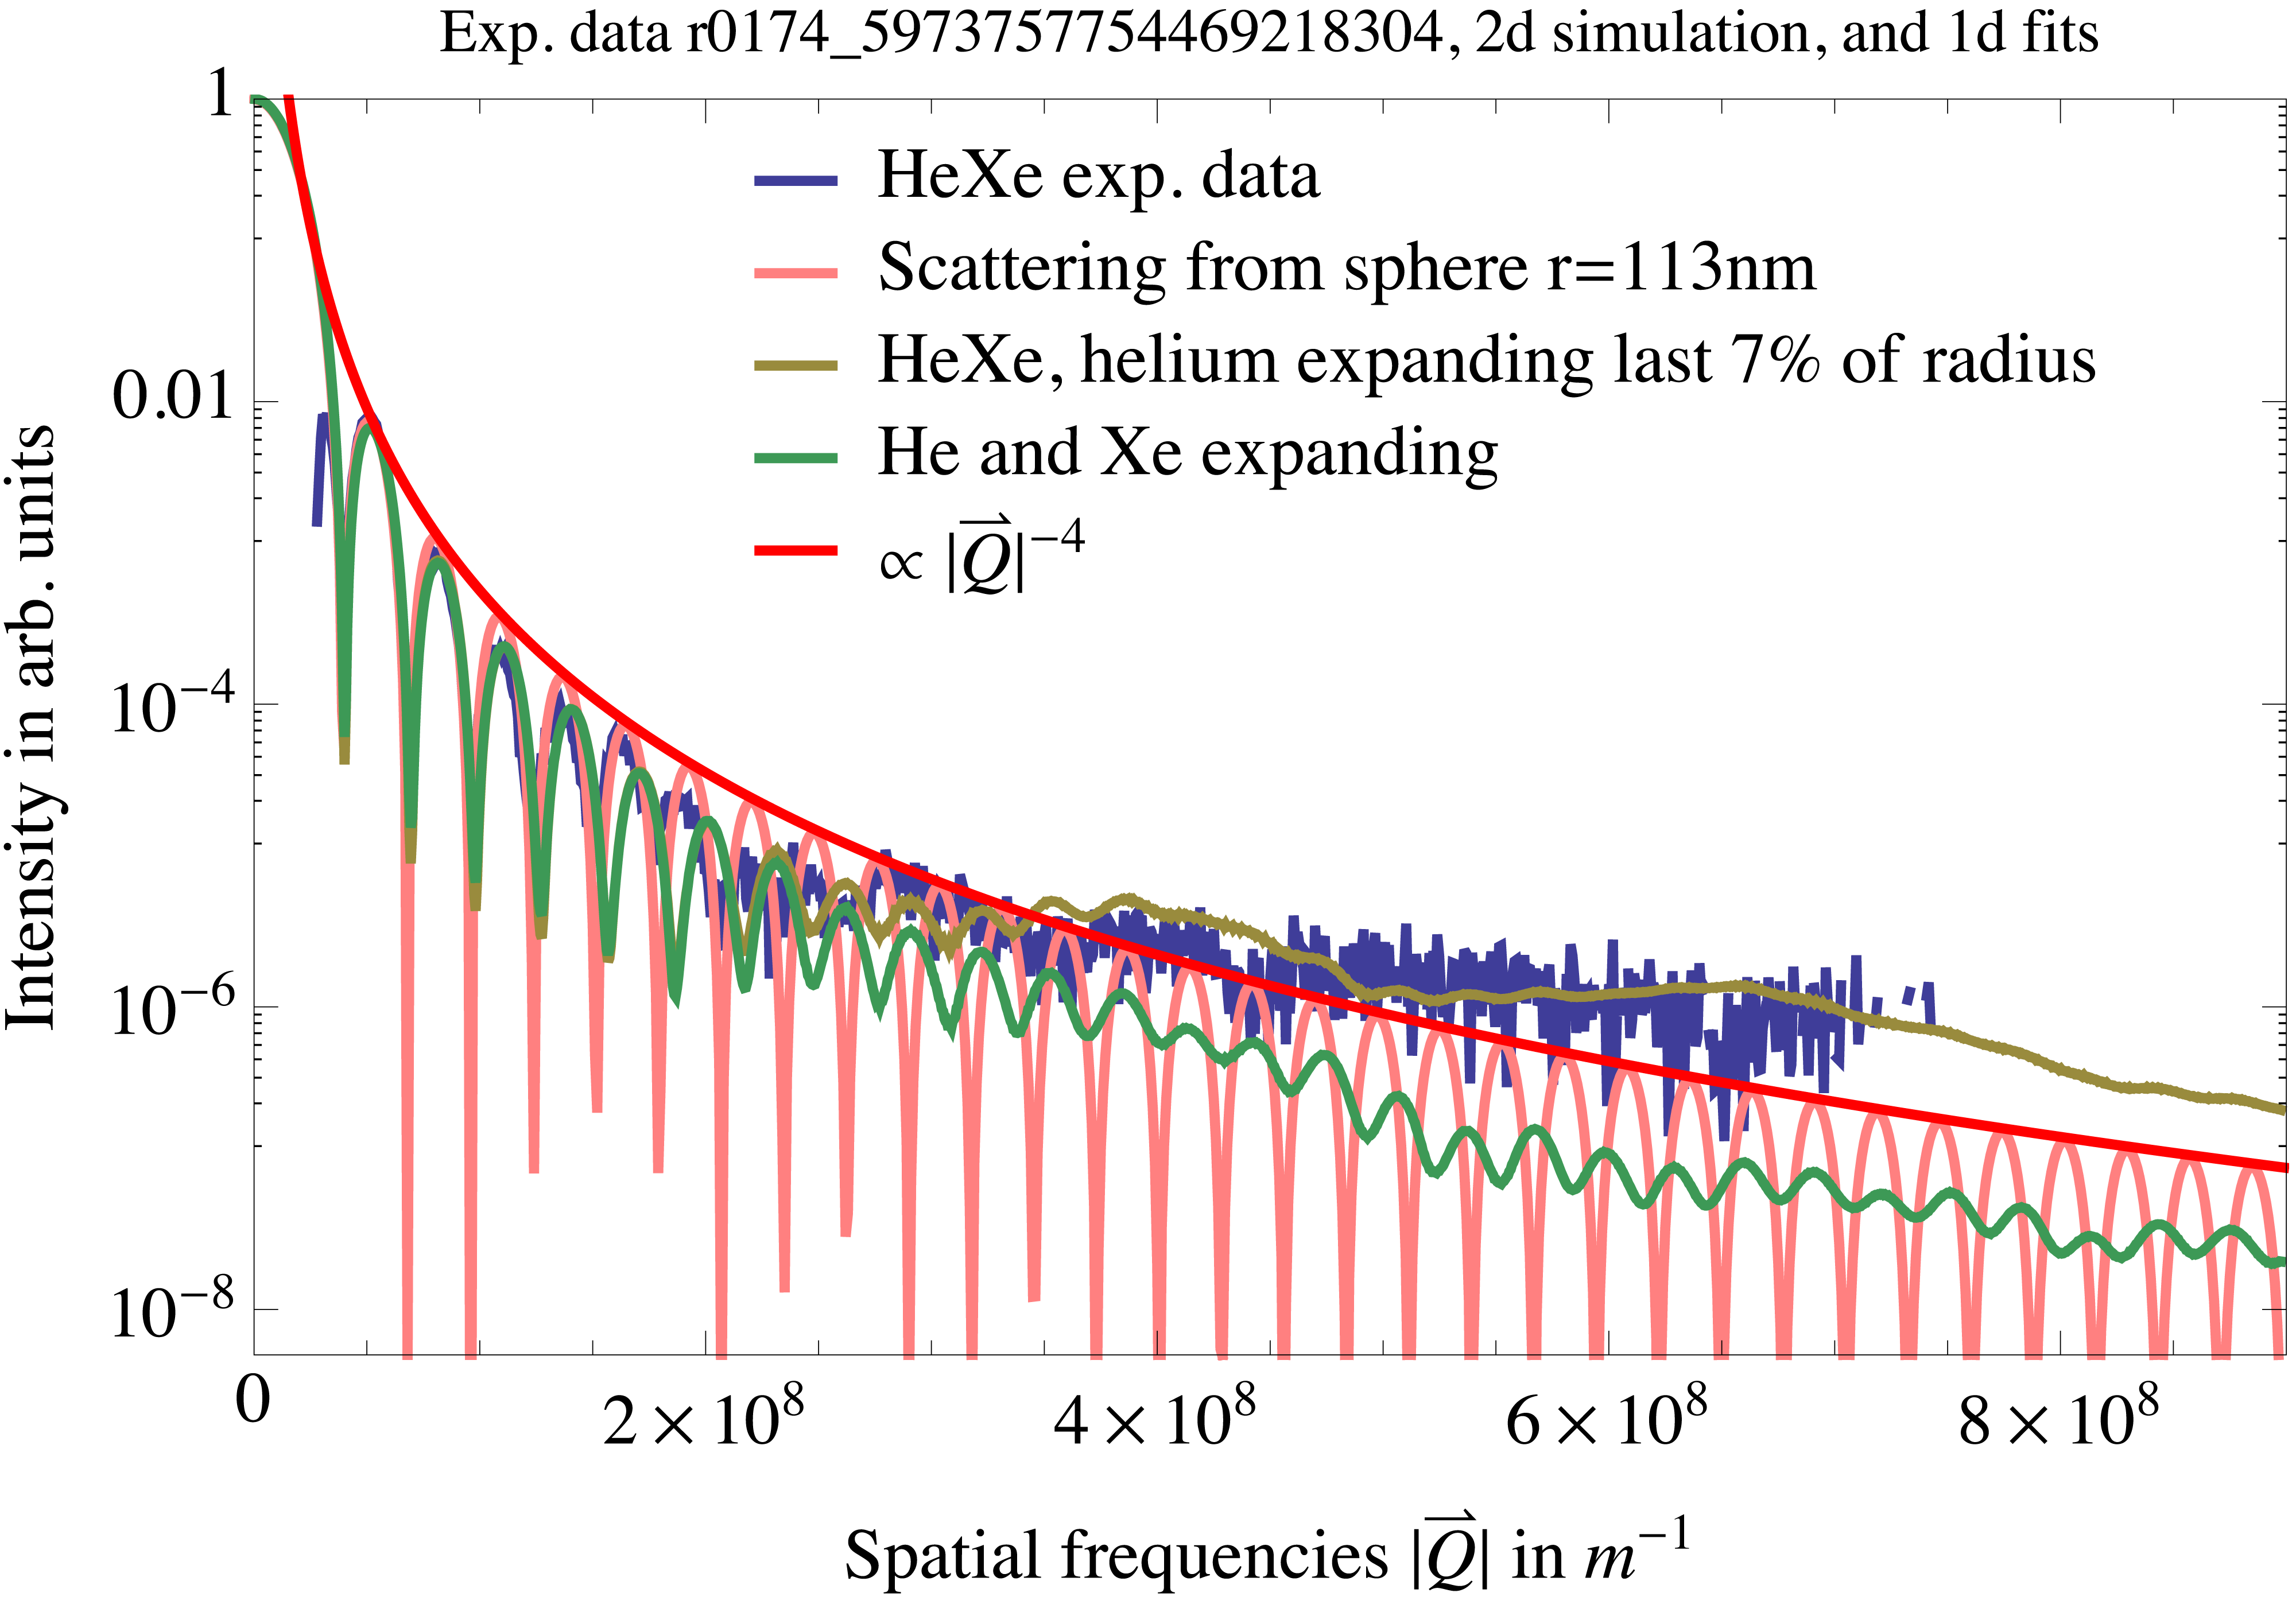
\includegraphics[height=6.0cm]{images/results/HeXe-cluster-113-0-5-doping2.png}
	\caption[Simulation and exp. data: Structural damage in He-droplet.]{Matching experimental data of HeXe-clusters with $r_{\text{He}}\approx \SI{113}{\nano\meter}$ at $\Delta t=\SI{800}{\femto\second}$ and simulations. a) The measured diffraction pattern has been projected to 1D (blue curve). b) From the same data, a 2D reconstruction of the HeXe-cluster is performed. c) The reconstruction is used to construct the simulated electron densities. These are then Fourier transformed and compared to the experimental data in a). Here, several simulated cases are shown and labeled in the legend of a). The simulation of an expanding He-droplet with an intact Xe-cluster fit the experimental data best (yellow curve).}
	\label{fig:HeXe-cluster-113-0.5}
\end{figure}
Let us use these insights to compare the 2D-simulations to the measured diffraction patterns. Figure \ref{fig:HeXe-cluster-113-0.5} matches the experimental diffraction data and simulations: The blue curve in Figure \ref{fig:HeXe-cluster-113-0.5}a) is the measured diffraction data projected to 1D; Figure \ref{fig:HeXe-cluster-113-0.5}b) shows the corresponding HeXe-cluster reconstruction in 2D; Figure \ref{fig:HeXe-cluster-113-0.5}c) shows a 2D electron density model that has been constructed to match the 2D reconstruction; and again Figure \ref{fig:HeXe-cluster-113-0.5}a) shows the 1D diffraction patterns from the simulated electron densities. These experimental data have been taken at a time delay $\Delta t=$ \SI{800}{\femto\second}. The HeXe-cluster has a radius $r_{He}\approx$ \SI{113}{\nano\meter}. The dense spots in the reconstruction have been simulated with \num{9} Xe-clusters of radii $r_{Xe}=$ \SIlist{4;4;4;4;3;0.5;0.5;0.5;0.5}{\nano\meter}. These radii of the simulated Xe-clusters have been determined iteratively such that a Xe-doping level of \SI{\sim 0.5}{\percent} was reached in the simulations -- for clarity, the experimental Xe-doping level is also \SI{\sim 0.5}{\percent}. In the diffraction pattern, the scattering of a sphere with a radius $r=$ \SI{113}{\nano\meter} (pink line) and its envelope (red line) are shown as a comparison. The yellow curve is a simulated diffraction pattern that shows an expanding He-droplet, where the last \SI{7}{\percent} of the shell is exponentially expanding, while the Xe-clusters stay intact. The green curve shows the simulated diffraction pattern, where the He-droplet is expanding at the last \SI{7}{\percent} of its radius and - to make the dependency clear - \SI{90}{\percent} of the Xe-clusters outer radii are expanding. The simulations show a very good agreement with the expanding He-droplet at low spatial-frequencies $\lvert\vec{Q}\rvert$. At high frequencies, only the yellow curve that uses intact Xe-clusters in the simulation reproduces the measured diffraction pattern well.\\[1\baselineskip]
%
The above HeXe-cluster simulations show that sample damage leaves a distinct feature in the diffraction pattern corresponding to either the expanding He-droplet or the expanding Xe-clusters. The measured diffraction pattern is fitted best using the electron density model of an expanding He-droplet and intact Xe-clusters. This indicates that helium acts as sacrificial layer slowing the nanoplasma expansion of the Xe-clusters, as xenon is the dominant photon absorber. Charge and kinetic energy transfer \cite{Hau-Riege-2007-PRL,Hoener-2008-JPB} from the Xe-cluster to the He-droplet, as discussed in more detail in Section \ref{sec:hexe--and-he-TOF}, could lead to a surface softening He-droplet but intact Xe-clusters. It should be noted, however, that sample damage in the Xe-clusters could be still possible but may not be detectable due to current resolution limitations.
%
%Summarizing, real-space reconstructions of the HeXe-cluster, as well as 2D-simulations that have been compared to the diffraction images indicate that HeXe-cluster arrange as plum-pudding core--shell system with few Xe-clusters. Furthermore, the 2D simulations indicate that the He- and Xe-cluster contribute distinctly to low- and high-spatial-frequencies, respectively. Therefore, if either the He- or Xe-clusters of the HeXe-cluster undergo a surface softening it shows distinctly in the scattering pattern.
%
%
%
\subsection{Sacrificial layers: Comparison of sample damage in HeXe-cluster}\label{sec:comparison-of-He-and-HeXe-clusters}
%%%%%%%%%%%%%%%%%%%%
% Start with helium - diff pattern
% Show several HeXe - diff patterns
% Compare...
%%%%%%%%%%%%%%%%%%%%%%
%
\begin{figure}
	\centering
		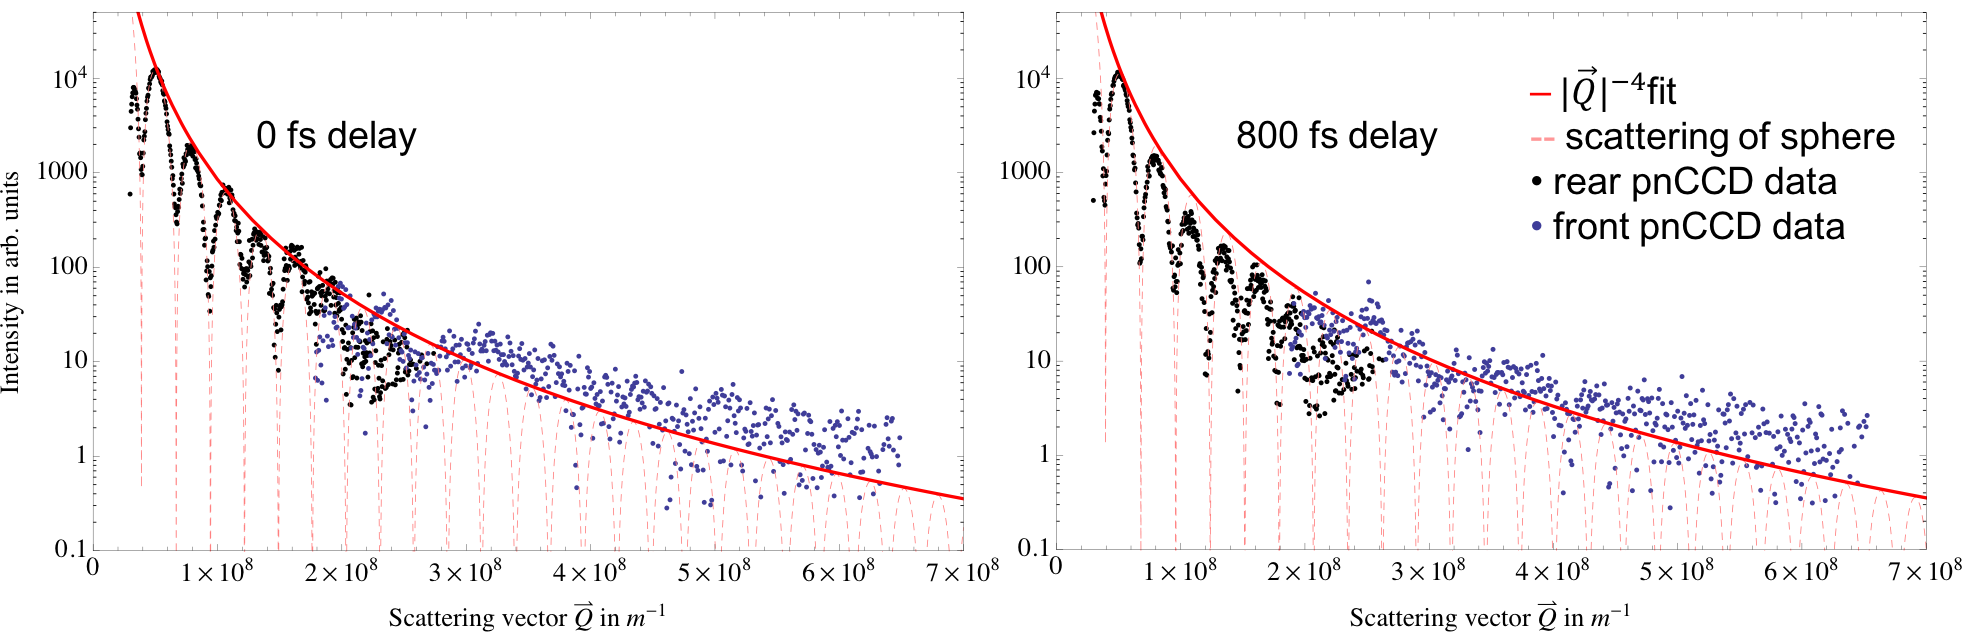
\includegraphics[width=1.00\textwidth]{images/results/HeXe-comparison-0-800-fs.png}
	\caption[Single-shot diffraction patterns of HeXe-cluster at different time delays]{Single-shot diffraction pattern of HeXe-cluster at time delays $\Delta t =$ 
	\SIlist{0;800}{\femto\second}. At $\Delta t=0$ fs, the diffraction pattern follows the scattering pattern of a sphere at low spatial-frequencies but stays well above the envelope function $\lvert\vec{Q}\rvert^{-4}$ at high spatial-frequencies. At $\Delta t=$ \SI{800}{\femto\second}, the scattering curve deviates from the scattering pattern of a sphere at low spatial-frequencies indicating X-ray induced damage to the He-shell structure. At high spatial frequencies, the signal changes little compared to the $\Delta t=$ \SI{0}{\femto\second} data, which indicates that the Xe is undamaged.
	%indicating intact Xe-cluster, i.e., cores. This suggests that the He-droplet functions as sacrificial shell keeping the Xe-nanoparticles intact. More in text.
	}
	\label{fig:HeXe-comparison-0-800-fs}
\end{figure}
%
Now that we have discussed the distinct features of sample damage in plum-pudding type HeXe-clusters in Section \ref{sec:helium-xenon-data}, we can analyze the scattering response of HeXe-cluster in another way. In a first step, this section compares the measured scattering response of HeXe-clusters at $\Delta t=\SI{0}{\femto\second}$ to the response at  $\Delta t=\SI{800}{\femto\second}$. And in a second step, the HeXe-clusters are compared to the time-resolved scattering response of pristine He- and Xe-clusters.\\[1\baselineskip]
%
Starting with the HeXe-clusters, single-shot diffraction images of HeXe-cluster with radii $r_{\text{He}}\approx$ \SIlist{116;113.5}{\nano\meter}, at time delays $\Delta t =$ \SIlist{0;800}{\femto\second}, respectively, are shown in Figure \ref{fig:HeXe-comparison-0-800-fs}. The experimental data for $\Delta t =$ \SI{800}{\femto\second} is the same as in Figure \ref{fig:HeXe-cluster-113-0.5}. The black dots are data points from the rear pnCCD and the blue dots are data points from the front pnCCD. The pink, dashed curve is the scattering from a sphere fitted to the first order of diffraction and the red curve is its envelope. 
For $\Delta t=$\SI{0}{\femto\second}, the rear pnCCD data points agree well with the scattering of intact He-droplets (compare to pink, dashed line). The data points from the front detector lay well above the scattering envelope function of the sphere, which corresponds to the scattering of intact Xe-clusters (compare Section \ref{sec:helium-xenon-data}). For $\Delta t =$ \SI{800}{\femto\second} - as already discussed in Section \ref{sec:helium-xenon-data} - the low spatial frequency intensity contributions agree well with the scattering of a damaged He-droplet, while the high spatial frequencies intensities can be best fitted with intact Xe-clusters. The single-shot events at $\Delta t=$ \SIlist{0;800}{\femto\second} allow us now to identify their differences and the main difference is that the He-droplet's low spatial frequency contributions in the intensity distribution are reduced. The high spatial frequency contributions to the intensity distribution that originate dominantly from the Xe-clusters are affected little, as we will see in more detail below.\\[1\baselineskip]
%
\begin{table}%
\centering
\textbf{Measured scattering / expected scattering}\\
\begin{tabular}{ | c || c | c | }
\hline
	 &\multicolumn{2}{c|}{\textbf{At time delay $\Delta t$}} \\
	\textbf{For sample} & \SI{0}{\femto\second}  & \SI{800}{\femto\second} \\ \hline \hline
	Xe-cluster & \num{0.91} & \num{0.26} \\ \hline
	He-droplet & \num{0.89} & \num{0.65} \\ \hline
	HeXe-cluster & $1$ & \num{1.33} \\ \hline
	%Xe-cluster & \num{0.91 \pm 0.1} & \num{0.26 \pm  0.1} \\ \hline
	%He-droplet & \num{0.89 \pm 0.1} & \num{0.65\pm   0.1} \\ \hline
	%HeXe-cluster & $1$ & \num{1.33 \pm  0.33} \\ \hline
\end{tabular}
\caption[Relative comparison of measured scattering versus expected scattering.]{Relative comparison of measured scattering versus expected scattering for Xe-, He- and HeXe-cluster at large spatial frequencies.}
\label{tab:he-vs-xe-vs-hexe-summary}
\end{table}
%
Let us quantify the intensity contributions at high spatial frequencies now in more detail to analyze potential sample damage of the embedded Xe-clusters. Previous studies have used a so-called R-factor (e.g., Reference \cite{Neutze-2000-Nature,Hau-Riege-2008-PRE}) that successfully quantified effects of radiation damage in computer simulations. In the following, a comparison of the measured scattering versus the expected scattering is made and the results of this comparison are summarized in Table \ref{tab:he-vs-xe-vs-hexe-summary}. To start with, let us analyze pristine He- and Xe-clusters first. The diffraction patterns of pristine He- or Xe-clusters can be easily compared to the scattering curve of a sphere. The scattering of a curve of a sphere is here denoted as the function $i(\vec{Q})$. We can also introduce a function $h(\vec{Q})$ that interpolates between the data points of pristine He- and Xe-cluster. The relative difference of these functions at a certain time delay can be noted as $\tfrac{\sum{h(\vec{Q}})}{\sum{i(\vec{Q})}}|_{\Delta t}^{\text{sample}}$, with the sums over $\lvert \vec{Q}\rvert$ running between \SIrange[scientific-notation = fixed, fixed-exponent = 8]{2.8e8}{6.4e8}{\per\meter}. For Xe- and He-clusters at $\Delta t =$ \SI{0}{\femto\second}, we find values close to the expected scattering. The measured scattering divided by the expected scattering is $\SI{91}{\percent} |_{\Delta t = 0 \text{fs}}^{\text{Xe}}$ and $\SI{89}{\percent}|_{\Delta t=0 \text{fs}}^{\text{He}}$. The interpolating function underestimates the actual scattering by \SI{\sim 10}{\percent}, which gives us an idea of the uncertainty of this estimate. For the delay $\Delta t=$ \SI{800}{\femto\second}, the actual scattering is reduced due to the surface softening such that $\SI{26}{\percent} |_{\Delta t = 800 \text{fs}}^{\text{Xe}}$ and $\SI{65}{\percent} |_{\Delta t = 800 \text{fs}}^{\text{Xe}}$ (compare to Section \ref{sec:xenon-data} and \ref{sec:He-data-real}). HeXe-clusters cannot directly be compared to the scattering of a sphere. However, we may compare similar single-shot events at different time delays to each other. The two single-shot events for $\Delta t=$ \SIlist{0;800}{\femto\second} that are shown in Figure \ref{fig:HeXe-comparison-0-800-fs} represent similar single events, as they have the same incident beam intensity, $I_{0}$, in the $I_{0} \lvert\vec{Q}\rvert^{-4}$ fit, a size difference of only \SI{\sim 2}{\percent}, and are produced at the same source and doping conditions. When comparing the interpolating functions $h(\vec{Q}) |_{\Delta t = 800 \text{fs}}^{\text{HeXe}}/h(\vec{Q}) |_{\Delta t = 0 \text{fs}}^{\text{HeXe}}$ at different time delays $\Delta t$, \SI{33}{\percent} more scattering at large $\lvert\vec{Q}\rvert$-values is measured. While the uncertainty in this shot-to-shot comparison is drastically higher, this estimate supports the finding that intensities at large spatial-frequencies are not reduced.\\[1\baselineskip] 
%This leads to yet another indicator that Xe-clusters exhibit no measurable X-ray induced damage despite the fact that sample damage in the He-droplet is visible at low spatial-frequencies $\lvert\vec{Q}\rvert$. 
%The source of uncertainty in this estimation likely originates from a varying pickup pattern of Xe-atoms and the uncertainty must be at least \SI{\sim 30}{\percent}.\\[1\baselineskip]
%
Summarizing, we find a reduction in scattering intensity at the spatial-frequencies $\lvert \vec{Q}\rvert=$ \SIrange[scientific-notation = fixed, fixed-exponent = 8]{2.8e8}{6.4e8}{\per\meter} of \SI{\sim 65}{\percent} in Xe-clusters and \SI{\sim 24}{\percent} in He-droplets \SI{800}{\femto\second} after the LCLS pump-pulse. These changes can be attributed to X-ray induced sample damage. If Xe-clusters are embedded in a He-droplet, no scattering reduction can be measured \SI{800}{\femto\second} after the pump-pulse. This indicates that embedded or tampered Xe-clusters exhibit no measurable sample damage at the current resolution. However, the He-droplet shows X-ray induced damage in the diffraction image. This indicates that in HeXe-clusters the He-droplet acts as sacrificial layer slowing indications of Xe-cluster sample damage in diffraction images. As discussed in previous sections in  more detail, charge and kinetic energy transfer \cite{Hau-Riege-2007-PRL,Hoener-2008-JPB} are likely responsible for the sample integrity of the dominantly absorbing Xe-clusters.
%The He-droplet appears to shed atomic layers, which transports energy away from the Xe-clusters and enables them to exhibit no measurable damage patterns that were discussed in Section \ref{sec:helium-xenon-data}.
%
%
%
%\subsection{Time-of-flight data of helium-xenon core-shell systems}
%%%%%%%%%%%%%%%%%%%%%%%%%%%%%%%%%%%%%%%%%%%%%%%%%%%
%- Show dynamics of XeHe data in tof trace.\\
%- More hefty nanoplasma expansion in HeXe than in raw He.\\
%- Complement with simulations from Phay.
%%%%%%%%%%%%%%%%%%%%%%%%%%%%%%%%%%%%%%%%%%%%%%%%%%%
%
%
%
%\subsection{Diffraction images of helium-xenon core shell systems}
%%%%%%%%%%%%%%%%%%%%%%%%%%%%%%%%%%%%%%%%%%%%%%%%%
%- Discuss diffraction images\\
%- Show how scattering intensity drops from He signal but not from Xe signal.\\
%- Eventually subsection for reconstructions.
%%%%%%%%%%%%%%%%%%%%%%%%%%%%%%%%%%%%%%%%%%%%%%%%%
%
%
%
%\subsection{Core-shell system considerations}
%
%
%
%\section{Static data}\label{sec:static}
%%%%%%%%%%%%%%%%%%%%%%%%%%%%%%%%%%%%%%%%%%
%-Include in other studies? Or appendix?
%%%%%%%%%%%%%%%%%%%%%%%%%%%%%%%%%%%%%%%%%%%%
%
%
%
%\section{Discussion and conclusion of the X-ray pump--X-ray probe study}
%%%%%%%%%%%%%%%%%%%%%%%%%%%%%%%%%%%%%%%%
%- Conclusion where the results are compared to each other\\
%- This experiment shows that heterogeneous clusters, as in tampered layers, do inhibit radiation damage of the sample target while the sacrificial layer undergoes a rapid nanoplasma transition.
%%%%%%%%%%%%%%%%%%%%%%%%%%%%%%%%%%%%%%%%%%
%The X-ray pump--X-ray probe study reveals some induced dynamics in Xe- and HeXe-cluster. In pristine Xe-cluster, we observe the nanoplasma expansion in the diffraction patternsa nd we can compare the results to other pump--probe studies using optical pump laser. The absorbed energy by the Xe-cluster is comparable in the optical to X-ray study (TBD), which is most relevant for the extend of the nanoplasma expansion. The time-of-flight spectroscopy reveals a to optical laser hidden resonance that is likely due to relaxation processes in the highly excited atoms. As an inner shell electron is ionized a chemical shift changes the ionization potentials and dynamic relaxation processes allow the absorption of more photons at certain stages \citep{Ho-2014-PRL}.\\
%Heterogeneous HeXe-cluster, doped using the pickup-principle, arrange in a plum-pudding type model, where Xe atoms form few Xe-cluster within one large (superfluid) He-droplet. 2D-simulations furthermore show that the X-ray induced dynamics in HeXe-cluster manifest only in the He-droplet.
%
%
%